\documentclass[openany]{book}
\usepackage{lmodern}
\usepackage{amssymb,amsmath}
\usepackage{ifxetex,ifluatex}
\usepackage{fixltx2e} % provides \textsubscript
\ifnum 0\ifxetex 1\fi\ifluatex 1\fi=0 % if pdftex
  \usepackage[T1]{fontenc}
  \usepackage[utf8]{inputenc}
\else % if luatex or xelatex
  \ifxetex
    \usepackage{mathspec}
  \else
    \usepackage{fontspec}
  \fi
  \defaultfontfeatures{Ligatures=TeX,Scale=MatchLowercase}
\fi
% use upquote if available, for straight quotes in verbatim environments
\IfFileExists{upquote.sty}{\usepackage{upquote}}{}
% use microtype if available
\IfFileExists{microtype.sty}{%
\usepackage{microtype}
\UseMicrotypeSet[protrusion]{basicmath} % disable protrusion for tt fonts
}{}
\usepackage[margin=1in]{geometry}
\usepackage{hyperref}
\hypersetup{unicode=true,
            pdftitle={Homework One},
            pdfauthor={Vinicio Haro; Sang Yoon (Andy) Hwang; Julian McEachern; Jeremy O'Brien; Bethany Poulin},
            pdfborder={0 0 0},
            breaklinks=true}
\urlstyle{same}  % don't use monospace font for urls
\usepackage{natbib}
\bibliographystyle{apalike}
\usepackage{color}
\usepackage{fancyvrb}
\newcommand{\VerbBar}{|}
\newcommand{\VERB}{\Verb[commandchars=\\\{\}]}
\DefineVerbatimEnvironment{Highlighting}{Verbatim}{commandchars=\\\{\}}
% Add ',fontsize=\small' for more characters per line
\usepackage{framed}
\definecolor{shadecolor}{RGB}{248,248,248}
\newenvironment{Shaded}{\begin{snugshade}}{\end{snugshade}}
\newcommand{\AlertTok}[1]{\textcolor[rgb]{0.94,0.16,0.16}{#1}}
\newcommand{\AnnotationTok}[1]{\textcolor[rgb]{0.56,0.35,0.01}{\textbf{\textit{#1}}}}
\newcommand{\AttributeTok}[1]{\textcolor[rgb]{0.77,0.63,0.00}{#1}}
\newcommand{\BaseNTok}[1]{\textcolor[rgb]{0.00,0.00,0.81}{#1}}
\newcommand{\BuiltInTok}[1]{#1}
\newcommand{\CharTok}[1]{\textcolor[rgb]{0.31,0.60,0.02}{#1}}
\newcommand{\CommentTok}[1]{\textcolor[rgb]{0.56,0.35,0.01}{\textit{#1}}}
\newcommand{\CommentVarTok}[1]{\textcolor[rgb]{0.56,0.35,0.01}{\textbf{\textit{#1}}}}
\newcommand{\ConstantTok}[1]{\textcolor[rgb]{0.00,0.00,0.00}{#1}}
\newcommand{\ControlFlowTok}[1]{\textcolor[rgb]{0.13,0.29,0.53}{\textbf{#1}}}
\newcommand{\DataTypeTok}[1]{\textcolor[rgb]{0.13,0.29,0.53}{#1}}
\newcommand{\DecValTok}[1]{\textcolor[rgb]{0.00,0.00,0.81}{#1}}
\newcommand{\DocumentationTok}[1]{\textcolor[rgb]{0.56,0.35,0.01}{\textbf{\textit{#1}}}}
\newcommand{\ErrorTok}[1]{\textcolor[rgb]{0.64,0.00,0.00}{\textbf{#1}}}
\newcommand{\ExtensionTok}[1]{#1}
\newcommand{\FloatTok}[1]{\textcolor[rgb]{0.00,0.00,0.81}{#1}}
\newcommand{\FunctionTok}[1]{\textcolor[rgb]{0.00,0.00,0.00}{#1}}
\newcommand{\ImportTok}[1]{#1}
\newcommand{\InformationTok}[1]{\textcolor[rgb]{0.56,0.35,0.01}{\textbf{\textit{#1}}}}
\newcommand{\KeywordTok}[1]{\textcolor[rgb]{0.13,0.29,0.53}{\textbf{#1}}}
\newcommand{\NormalTok}[1]{#1}
\newcommand{\OperatorTok}[1]{\textcolor[rgb]{0.81,0.36,0.00}{\textbf{#1}}}
\newcommand{\OtherTok}[1]{\textcolor[rgb]{0.56,0.35,0.01}{#1}}
\newcommand{\PreprocessorTok}[1]{\textcolor[rgb]{0.56,0.35,0.01}{\textit{#1}}}
\newcommand{\RegionMarkerTok}[1]{#1}
\newcommand{\SpecialCharTok}[1]{\textcolor[rgb]{0.00,0.00,0.00}{#1}}
\newcommand{\SpecialStringTok}[1]{\textcolor[rgb]{0.31,0.60,0.02}{#1}}
\newcommand{\StringTok}[1]{\textcolor[rgb]{0.31,0.60,0.02}{#1}}
\newcommand{\VariableTok}[1]{\textcolor[rgb]{0.00,0.00,0.00}{#1}}
\newcommand{\VerbatimStringTok}[1]{\textcolor[rgb]{0.31,0.60,0.02}{#1}}
\newcommand{\WarningTok}[1]{\textcolor[rgb]{0.56,0.35,0.01}{\textbf{\textit{#1}}}}
\usepackage{longtable,booktabs}
\usepackage{graphicx,grffile}
\makeatletter
\def\maxwidth{\ifdim\Gin@nat@width>\linewidth\linewidth\else\Gin@nat@width\fi}
\def\maxheight{\ifdim\Gin@nat@height>\textheight\textheight\else\Gin@nat@height\fi}
\makeatother
% Scale images if necessary, so that they will not overflow the page
% margins by default, and it is still possible to overwrite the defaults
% using explicit options in \includegraphics[width, height, ...]{}
\setkeys{Gin}{width=\maxwidth,height=\maxheight,keepaspectratio}
\IfFileExists{parskip.sty}{%
\usepackage{parskip}
}{% else
\setlength{\parindent}{0pt}
\setlength{\parskip}{6pt plus 2pt minus 1pt}
}
\setlength{\emergencystretch}{3em}  % prevent overfull lines
\providecommand{\tightlist}{%
  \setlength{\itemsep}{0pt}\setlength{\parskip}{0pt}}
\setcounter{secnumdepth}{0}

%%% Use protect on footnotes to avoid problems with footnotes in titles
\let\rmarkdownfootnote\footnote%
\def\footnote{\protect\rmarkdownfootnote}

%%% Change title format to be more compact
\usepackage{titling}

% Create subtitle command for use in maketitle
\providecommand{\subtitle}[1]{
  \posttitle{
    \begin{center}\large#1\end{center}
    }
}

\setlength{\droptitle}{-2em}

  \title{Homework One}
    \pretitle{\vspace{\droptitle}\centering\huge}
  \posttitle{\par}
  \subtitle{Group Two}
  \author{Vinicio Haro \\ Sang Yoon (Andy) Hwang \\ Julian McEachern \\ Jeremy O'Brien \\ Bethany Poulin}
    \preauthor{\centering\large\emph}
  \postauthor{\par}
      \predate{\centering\large\emph}
  \postdate{\par}
    \date{15 October 2019}

\usepackage{booktabs}
\usepackage[table]{xcolor}

% set plain style for page numbers
\pagestyle{plain}
\raggedbottom

% change font
\usepackage{fontspec}
\setmainfont{Arial}

% remove "chapter" from chapter title
\usepackage{titlesec}
\titleformat{\chapter}
  {\normalfont\LARGE\bfseries}{\thechapter}{1em}{}
\titlespacing*{\chapter}{0pt}{3.5ex plus 1ex minus .2ex}{2.3ex plus .2ex}

% create color block quotes
\usepackage{tcolorbox}
\newtcolorbox{myquote}{colback=blue!5!white, colframe=blue!75!black}
\renewenvironment{quote}{\begin{myquote}}{\end{myquote}}

% wrap text
\usepackage{geometry}[textwidth=6in]

% kable 
\usepackage{tabu}
\usepackage{float}

\begin{document}
\maketitle

{
\setcounter{tocdepth}{1}
\tableofcontents
}
\hypertarget{overview}{%
\chapter*{Overview}\label{overview}}
\addcontentsline{toc}{chapter}{Overview}

We created this together, each member doing all of the problems and then voting on what to include and what to leave out of our final submission. In most cases, we used the guts of one members work and supplemented it with plots, metrics and interpretations from some or all other team member answers.

\hypertarget{dependencies}{%
\section{Dependencies}\label{dependencies}}

The following R packages were used in the completion of this work. Loading them all at the beggining should ensure that any code found in this document runs correctly.

\begin{Shaded}
\begin{Highlighting}[]
\CommentTok{#Textbook Packages}
\KeywordTok{library}\NormalTok{(fpp2)}
\KeywordTok{library}\NormalTok{(AppliedPredictiveModeling)}
\KeywordTok{library}\NormalTok{(mlbench)}

\CommentTok{#Processing}
\KeywordTok{library}\NormalTok{(tidyverse)}
\KeywordTok{library}\NormalTok{(RCurl)}
\KeywordTok{library}\NormalTok{(readxl)}

\CommentTok{#Graphing}
\KeywordTok{library}\NormalTok{(ggplot2)}
\KeywordTok{library}\NormalTok{(grid)}
\KeywordTok{library}\NormalTok{(gridExtra)}
\KeywordTok{library}\NormalTok{(lemon)}

\CommentTok{#Math}
\KeywordTok{library}\NormalTok{(tsfeatures)}
\KeywordTok{library}\NormalTok{(caret)}
\KeywordTok{library}\NormalTok{(forecast)}
\KeywordTok{library}\NormalTok{(randomForest)}
\KeywordTok{library}\NormalTok{(seasonal)}
\KeywordTok{library}\NormalTok{(psych)}
\KeywordTok{library}\NormalTok{(corrplot)}
\KeywordTok{require}\NormalTok{(e1071)}

\CommentTok{#Formatting}
\KeywordTok{library}\NormalTok{(knitr)}
\KeywordTok{require}\NormalTok{(default)}
\KeywordTok{library}\NormalTok{(kableExtra)}
\KeywordTok{library}\NormalTok{(magrittr)}
\end{Highlighting}
\end{Shaded}

\hypertarget{data-files}{%
\section{Data Files}\label{data-files}}

Where data is not included via an R package, and needs to be supplied , we referrenced a folder parallel to our code as such `/data/retail.xlsx'. In order for our code to read properly, you should create a parallel folder \texttt{data} to host such files.

\hypertarget{assignment-one}{%
\chapter{Assignment One}\label{assignment-one}}

\begin{itemize}
\tightlist
\item
  Hyndman 2.1\\
\item
  Hyndman 2.3
\end{itemize}

\hypertarget{hyndman-exercise-2.1}{%
\section{Hyndman Exercise 2.1}\label{hyndman-exercise-2.1}}

\begin{quote}
Use the help function to explore what the series \texttt{gold}, \texttt{woolyrnq} and \texttt{gas} represent.
\end{quote}

\begin{Shaded}
\begin{Highlighting}[]
\KeywordTok{data}\NormalTok{(}\StringTok{"gold"}\NormalTok{); }\CommentTok{#help("gold")}
\KeywordTok{data}\NormalTok{(}\StringTok{"woolyrnq"}\NormalTok{); }\CommentTok{#help("woolyrnq")}
\KeywordTok{data}\NormalTok{(}\StringTok{'gold'}\NormalTok{); }\CommentTok{#help("gas")}
\end{Highlighting}
\end{Shaded}

Per the \texttt{help} function, the \texttt{gold} series represents ``daily morning gold prices in US dollars. 1 January 1985-31 March 1989''; the \texttt{woolyrnq} series represents ``quarterly production of woollen yarn in Australia: tonnes. Mar 1965-Sep 1994''; and, the \texttt{gas} series represents ``Australian monthly gas production: 1956-1995.''

\hypertarget{a.-use-autoplot-to-plot-each-of-these-in-separate-plots.}{%
\subsection{\texorpdfstring{a. Use \texttt{autoplot()} to plot each of these in separate plots.}{a. Use autoplot() to plot each of these in separate plots.}}\label{a.-use-autoplot-to-plot-each-of-these-in-separate-plots.}}

The time plots below were generated from the \texttt{autoplot} function.

\hypertarget{gold}{%
\subsubsection{\texorpdfstring{\texttt{gold}}{gold}}\label{gold}}

\begin{Shaded}
\begin{Highlighting}[]
\NormalTok{p1 <-}\StringTok{ }\KeywordTok{autoplot}\NormalTok{(gold) }\OperatorTok{+}\StringTok{ }\KeywordTok{labs}\NormalTok{(}\DataTypeTok{title =} \StringTok{"Daily Morning Gold Prices"}\NormalTok{, }
  \DataTypeTok{subtitle =} \StringTok{"Time Series: 01 Jan 1985 - 31 Mar 1989"}\NormalTok{, }
  \DataTypeTok{x =} \StringTok{"Day"}\NormalTok{, }\DataTypeTok{y =} \StringTok{"Price (USD)"}\NormalTok{) }\OperatorTok{+}\StringTok{ }\KeywordTok{theme_bw}\NormalTok{() }\OperatorTok{+}\StringTok{ }\KeywordTok{theme}\NormalTok{()}

\NormalTok{p2 <-}\StringTok{ }\KeywordTok{ggAcf}\NormalTok{(gold) }\OperatorTok{+}\StringTok{ }\KeywordTok{labs}\NormalTok{(}\DataTypeTok{title =} \StringTok{""}\NormalTok{, }\DataTypeTok{subtitle =} \StringTok{"ACF Plot"}\NormalTok{) }\OperatorTok{+}\StringTok{ }
\StringTok{  }\KeywordTok{theme_bw}\NormalTok{() }\OperatorTok{+}\StringTok{ }\KeywordTok{theme}\NormalTok{()}

\KeywordTok{grid.arrange}\NormalTok{(p1, p2, }\DataTypeTok{nrow =} \DecValTok{1}\NormalTok{)}
\end{Highlighting}
\end{Shaded}

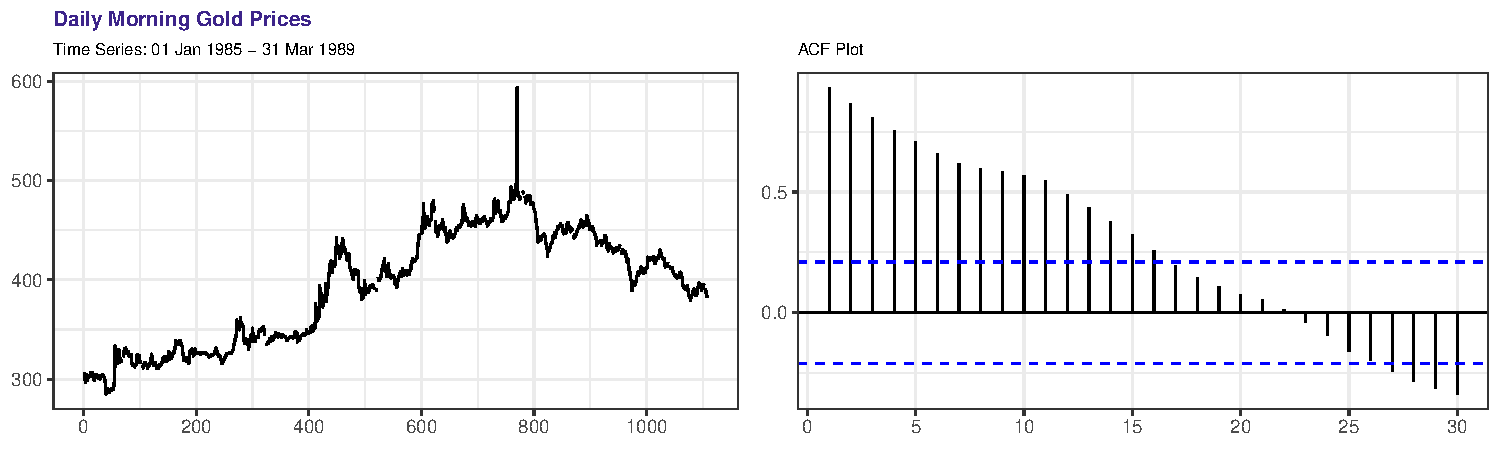
\includegraphics{homework-one_files/figure-latex/ha-2.1a-gold-1.pdf}

The \texttt{gold} series demonstrates a general, incremental trend until a large spike around day 775 (February 15, 1997). Thereafter the value of gold decreases over the remaining until the end of the timespan (March 31, 1989).

Based on the ACF plot, the trend increases until lag 22, after which it proceeds to decrease. The slightly scalloped shape between lags 5 and 10 suggest the possibility of some seasonality.

\hypertarget{woolyrnq}{%
\subsubsection{\texorpdfstring{\texttt{woolyrnq}}{woolyrnq}}\label{woolyrnq}}

\begin{Shaded}
\begin{Highlighting}[]
\NormalTok{p1 <-}\StringTok{ }\KeywordTok{autoplot}\NormalTok{(woolyrnq) }\OperatorTok{+}\StringTok{ }\KeywordTok{labs}\NormalTok{(}\DataTypeTok{title =} \StringTok{"Quarterly Australian Woollen Yarn Production"}\NormalTok{, }
  \DataTypeTok{subtitle =} \StringTok{"Time Series: Mar 1965 - Sep 1994"}\NormalTok{, }\DataTypeTok{x =} \StringTok{"Year"}\NormalTok{, }
  \DataTypeTok{y =} \StringTok{"Quantity (Tons)"}\NormalTok{) }\OperatorTok{+}\StringTok{ }\KeywordTok{theme_bw}\NormalTok{() }\OperatorTok{+}\StringTok{ }\KeywordTok{theme}\NormalTok{()}

\NormalTok{p2 <-}\StringTok{ }\KeywordTok{ggAcf}\NormalTok{(woolyrnq) }\OperatorTok{+}\StringTok{ }\KeywordTok{labs}\NormalTok{(}\DataTypeTok{title =} \StringTok{""}\NormalTok{, }\DataTypeTok{subtitle =} \StringTok{"ACF Plot"}\NormalTok{) }\OperatorTok{+}\StringTok{ }
\StringTok{  }\KeywordTok{theme_bw}\NormalTok{() }\OperatorTok{+}\StringTok{ }\KeywordTok{theme}\NormalTok{()}

\KeywordTok{grid.arrange}\NormalTok{(p1, p2, }\DataTypeTok{nrow =} \DecValTok{1}\NormalTok{)}
\end{Highlighting}
\end{Shaded}

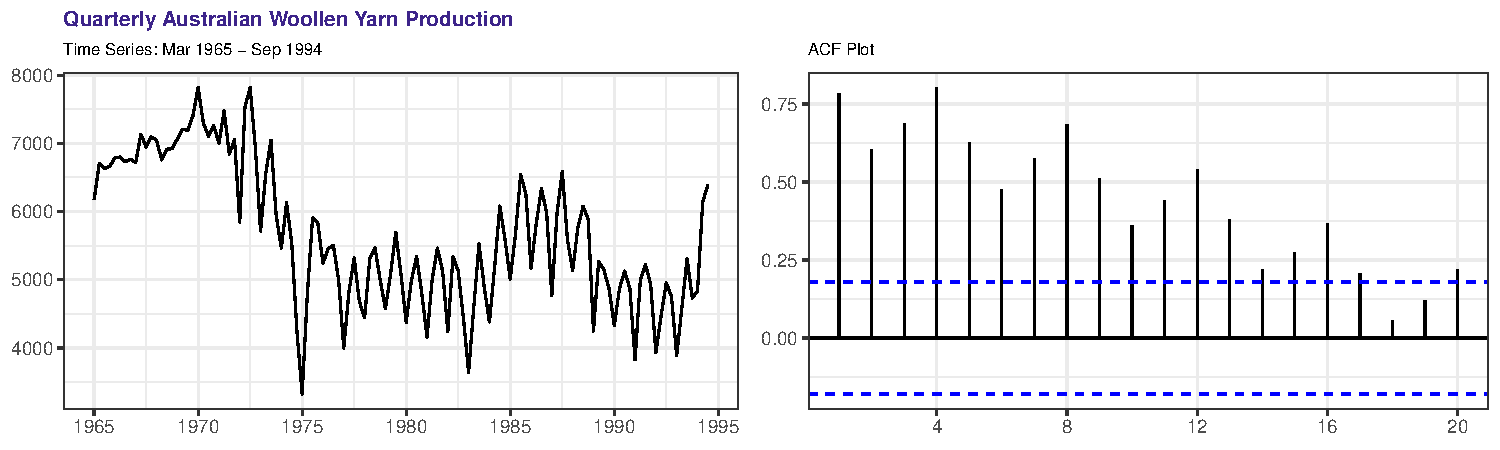
\includegraphics{homework-one_files/figure-latex/ha-2.1a-woolyrnq-1.pdf}
The \texttt{woolyrng} series exhibits a decremental trend, with a dramatic dip in early 1975.

The slight ``U'' shape repeating every 4 lags in the ACF plot suggests some seasonality, which can be described as mild cyclic behavior.

\hypertarget{gas}{%
\subsubsection{\texorpdfstring{\texttt{gas}}{gas}}\label{gas}}

\begin{Shaded}
\begin{Highlighting}[]
\NormalTok{p1 <-}\StringTok{ }\KeywordTok{autoplot}\NormalTok{(gas) }\OperatorTok{+}\StringTok{ }\KeywordTok{labs}\NormalTok{(}\DataTypeTok{title =} \StringTok{"Monthly Australian Gas Production"}\NormalTok{, }
  \DataTypeTok{subtitle =} \StringTok{"Time Series: 1956 - 1995"}\NormalTok{, }\DataTypeTok{x =} \StringTok{"Year"}\NormalTok{, }\DataTypeTok{y =} \StringTok{"Quantity"}\NormalTok{) }\OperatorTok{+}\StringTok{ }
\StringTok{  }\KeywordTok{theme_bw}\NormalTok{() }\OperatorTok{+}\StringTok{ }\KeywordTok{theme}\NormalTok{()}

\NormalTok{p2 <-}\StringTok{ }\KeywordTok{ggAcf}\NormalTok{(gas, }\DataTypeTok{lag =} \DecValTok{80}\NormalTok{) }\OperatorTok{+}\StringTok{ }\KeywordTok{labs}\NormalTok{(}\DataTypeTok{title =} \StringTok{""}\NormalTok{, }\DataTypeTok{subtitle =} \StringTok{"ACF Plot"}\NormalTok{) }\OperatorTok{+}\StringTok{ }
\StringTok{  }\KeywordTok{theme_bw}\NormalTok{() }\OperatorTok{+}\StringTok{ }\KeywordTok{theme}\NormalTok{()}

\KeywordTok{grid.arrange}\NormalTok{(p1, p2, }\DataTypeTok{nrow =} \DecValTok{1}\NormalTok{)}
\end{Highlighting}
\end{Shaded}

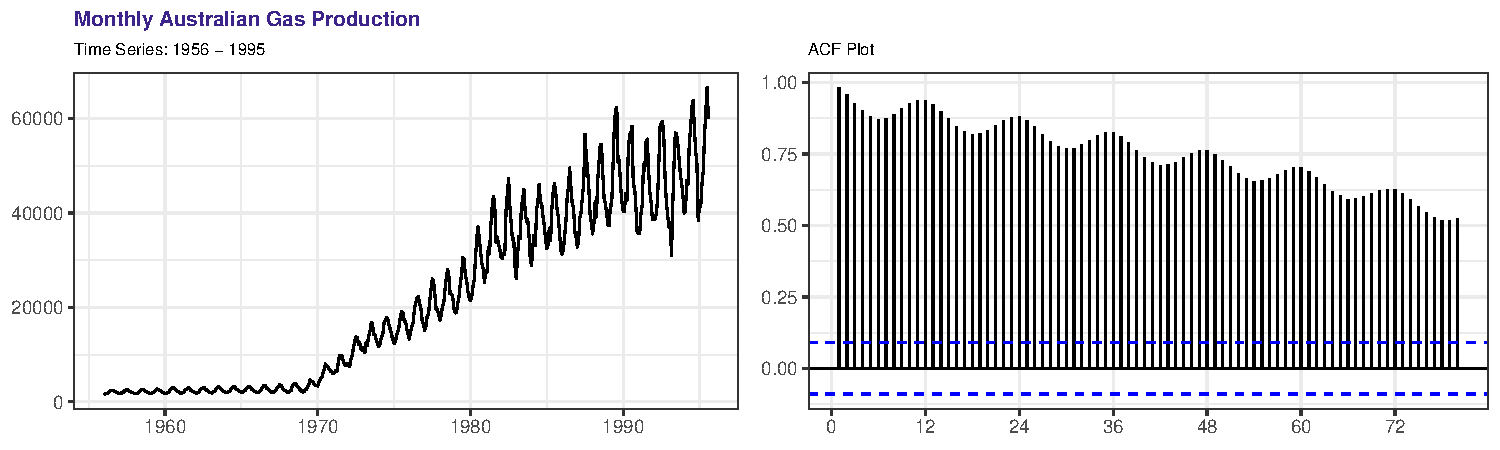
\includegraphics{homework-one_files/figure-latex/ha-2.1a-gas-1.pdf}

Lastly, the \texttt{gas} plot shows monthly changes to Australian gas production. As production takes off around 1970 in an overall increasing trend, the seasonal peaks and valleys also grow wider apart, suggesting a multiplicative relationship.

A moderate ``U'' shape repeats every 12 lags in the ACF plot, indicating a seasonal pattern.

\hypertarget{b.-what-is-the-frequency-of-each-series-hint-apply-the-frequency-function.}{%
\subsection{\texorpdfstring{b. What is the frequency of each series? Hint: apply the \texttt{frequency()} function.}{b. What is the frequency of each series? Hint: apply the frequency() function.}}\label{b.-what-is-the-frequency-of-each-series-hint-apply-the-frequency-function.}}

\begin{Shaded}
\begin{Highlighting}[]
\KeywordTok{frequency}\NormalTok{(gold)}
\KeywordTok{frequency}\NormalTok{(woolyrnq)}
\KeywordTok{frequency}\NormalTok{(gas)}
\end{Highlighting}
\end{Shaded}

The frequency of timeseries shows us the number of observations within a singular seasonal pattern.

\begin{itemize}
\tightlist
\item
  \textbf{Gas Frequency:} 12\\
\item
  \textbf{Yarn Frequency:} 4
\item
  \textbf{Gold Frequency:} 1
\end{itemize}

The output of the \texttt{frequency} function indicates that \texttt{gold} is an annual time series, \texttt{woolyrnq} is a quarterly series, and \texttt{gas} is a monthly series.

\hypertarget{c.-use-which.max-to-spot-the-outlier-in-the-gold-series.-which-observation-was-it}{%
\subsection{\texorpdfstring{c. Use \texttt{which.max()} to spot the outlier in the gold series. Which observation was it?}{c. Use which.max() to spot the outlier in the gold series. Which observation was it?}}\label{c.-use-which.max-to-spot-the-outlier-in-the-gold-series.-which-observation-was-it}}

\begin{Shaded}
\begin{Highlighting}[]
\KeywordTok{which.max}\NormalTok{(gold)}
\end{Highlighting}
\end{Shaded}

The \texttt{which.max()} function returns the index of the maximum value in a series:

\textbf{Gold Maximum Value:} 770

This number aligns with the observed spike in gold price from the time series plot in part (a).

\hypertarget{hyndman-exercise-2.3}{%
\section{Hyndman Exercise 2.3}\label{hyndman-exercise-2.3}}

\begin{quote}
Download some monthly Australian retail data from the book website. These represent retail sales in various categories for different Australian states, and are stored in a MS-Excel file.
\end{quote}

\hypertarget{a.-you-can-read-the-data-into-r-with-the-following-script}{%
\subsection{a. You can read the data into R with the following script:}\label{a.-you-can-read-the-data-into-r-with-the-following-script}}

\begin{Shaded}
\begin{Highlighting}[]
\NormalTok{retaildata <-}\StringTok{ }\NormalTok{readxl}\OperatorTok{::}\KeywordTok{read_excel}\NormalTok{(}\StringTok{"data/retail.xlsx"}\NormalTok{, }\DataTypeTok{skip =} \DecValTok{1}\NormalTok{)}
\end{Highlighting}
\end{Shaded}

\emph{The second argument (skip=1) is required because the Excel sheet has two header rows.}

\hypertarget{b.-select-one-of-the-time-series-as-follows-but-replace-the-column-name-with-your-own-chosen-column}{%
\subsection{b. Select one of the time series as follows (but replace the column name with your own chosen column):}\label{b.-select-one-of-the-time-series-as-follows-but-replace-the-column-name-with-your-own-chosen-column}}

\begin{Shaded}
\begin{Highlighting}[]
\NormalTok{myts <-}\StringTok{ }\KeywordTok{ts}\NormalTok{(retaildata[, }\StringTok{"A3349335T"}\NormalTok{], }\DataTypeTok{frequency =} \DecValTok{12}\NormalTok{, }\DataTypeTok{start =} \KeywordTok{c}\NormalTok{(}\DecValTok{1982}\NormalTok{, }
  \DecValTok{4}\NormalTok{))}
\end{Highlighting}
\end{Shaded}

\hypertarget{c.-explore-your-chosen-retail-time-series-using-the-following-functions-autoplot-ggseasonplot-ggsubseriesplot-gglagplot-ggacf.}{%
\subsection{\texorpdfstring{c. Explore your chosen retail time series using the following functions: \texttt{autoplot()}, \texttt{ggseasonplot()}, \texttt{ggsubseriesplot()}, \texttt{gglagplot()}, \texttt{ggAcf()}.}{c. Explore your chosen retail time series using the following functions: autoplot(), ggseasonplot(), ggsubseriesplot(), gglagplot(), ggAcf().}}\label{c.-explore-your-chosen-retail-time-series-using-the-following-functions-autoplot-ggseasonplot-ggsubseriesplot-gglagplot-ggacf.}}

\hypertarget{autoplot}{%
\subsubsection{Autoplot}\label{autoplot}}

\begin{Shaded}
\begin{Highlighting}[]
\KeywordTok{autoplot}\NormalTok{(myts) }\OperatorTok{+}\StringTok{ }\KeywordTok{labs}\NormalTok{(}\DataTypeTok{title =} \StringTok{"Monthly Australian Book Retail Data: A3349335T"}\NormalTok{, }
  \DataTypeTok{subtitle =} \StringTok{"Time Plot: Apr 1982 - Dec 2013"}\NormalTok{, }\DataTypeTok{x =} \StringTok{"Year"}\NormalTok{, }
  \DataTypeTok{y =} \StringTok{"Sales"}\NormalTok{) }\OperatorTok{+}\StringTok{ }\KeywordTok{theme_bw}\NormalTok{() }\OperatorTok{+}\StringTok{ }\KeywordTok{theme}\NormalTok{()}
\end{Highlighting}
\end{Shaded}

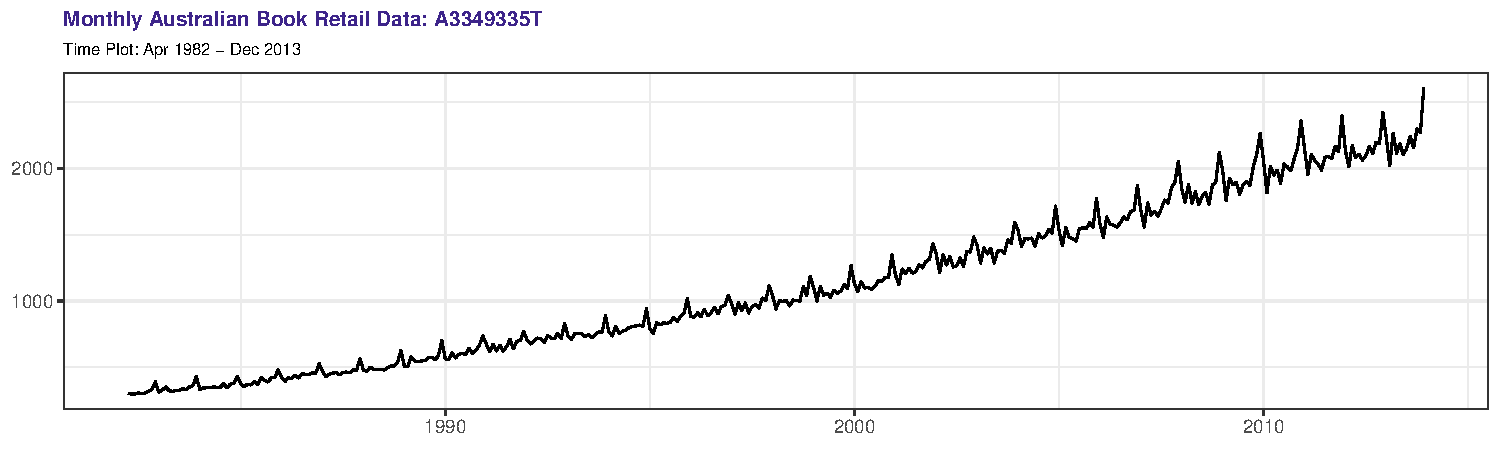
\includegraphics{homework-one_files/figure-latex/ha-2.3c-autoplot-1.pdf}

The output of the \texttt{autoplot} function demonstrate a general, incremental trend over the observed period, with a more pronounced peaks and valleys in the seasonal pattern.

\hypertarget{seasonal-plot}{%
\subsubsection{Seasonal Plot}\label{seasonal-plot}}

\begin{Shaded}
\begin{Highlighting}[]
\KeywordTok{ggseasonplot}\NormalTok{(myts, }\DataTypeTok{year.labels =} \OtherTok{TRUE}\NormalTok{, }\DataTypeTok{year.labels.left =} \OtherTok{TRUE}\NormalTok{) }\OperatorTok{+}\StringTok{ }
\StringTok{  }\KeywordTok{labs}\NormalTok{(}\DataTypeTok{title =} \StringTok{"Monthly Australian Book Retail Data: A3349335T"}\NormalTok{, }
    \DataTypeTok{subtitle =} \StringTok{"Seasonal Plot: Apr 1982 - Dec 2013"}\NormalTok{, }
    \DataTypeTok{x =} \StringTok{"Month"}\NormalTok{, }\DataTypeTok{y =} \StringTok{"Sales"}\NormalTok{) }\OperatorTok{+}\StringTok{ }\KeywordTok{theme_bw}\NormalTok{() }\OperatorTok{+}\StringTok{ }\KeywordTok{theme}\NormalTok{()}
\end{Highlighting}
\end{Shaded}

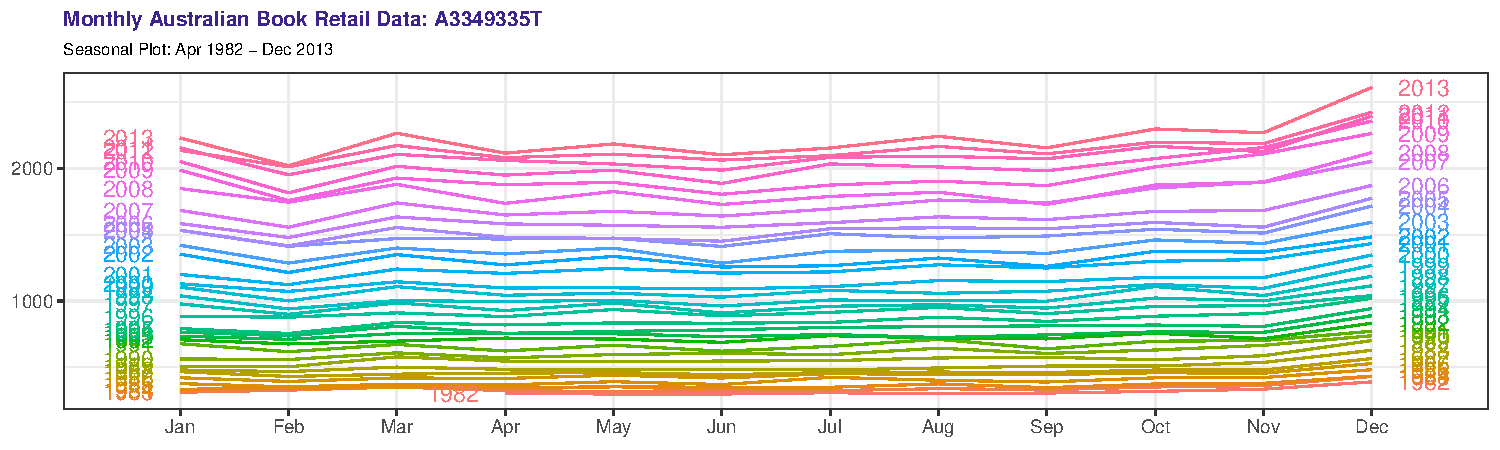
\includegraphics{homework-one_files/figure-latex/ha-2.3c-ggseasonplot-1.pdf}
Seasonal plots shows the observed data plotted for each year within the series. The seasons overlap to highlight underlying seasonal patterns and the years in which these trends occur. The seasonal plot below reveals that book sales tend to decline over January and February, rise in March and bump around over spring and summer before increasing over fall months into December. The overall increasing trend is evidenced by the roughly chronological progression in years on the right and left margins.

\hypertarget{subseries-plot}{%
\subsubsection{Subseries Plot}\label{subseries-plot}}

\begin{Shaded}
\begin{Highlighting}[]
\KeywordTok{ggsubseriesplot}\NormalTok{(myts) }\OperatorTok{+}\StringTok{ }\KeywordTok{labs}\NormalTok{(}\DataTypeTok{title =} \StringTok{"Monthly Australian Book Retail Data: A3349335T"}\NormalTok{, }
  \DataTypeTok{subtitle =} \StringTok{"Subseries Plot: Apr 1982 - Dec 2013"}\NormalTok{, }\DataTypeTok{x =} \StringTok{"Month"}\NormalTok{, }
  \DataTypeTok{y =} \StringTok{"Sales"}\NormalTok{) }\OperatorTok{+}\StringTok{ }\KeywordTok{theme_bw}\NormalTok{() }\OperatorTok{+}\StringTok{ }\KeywordTok{theme}\NormalTok{()}
\end{Highlighting}
\end{Shaded}

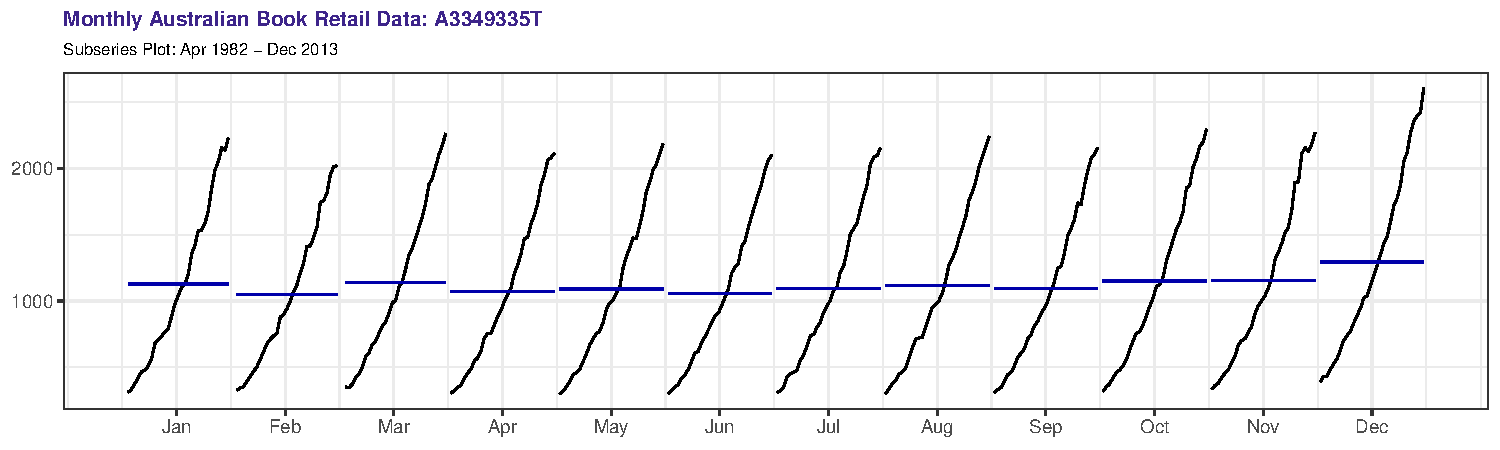
\includegraphics{homework-one_files/figure-latex/ha-2.3c-ggsubseriesplot-1.pdf}

The subseries plot provides a different way to view underlying seasonal patterns by separating each season in a year into an individual plot. The horizontal line shows the mean value of each month. The plot below reveals that, on average, the month of February sees the lowest sales and the month of December the highest over the observed time period.

\hypertarget{lag-plots}{%
\subsubsection{Lag Plots}\label{lag-plots}}

\begin{Shaded}
\begin{Highlighting}[]
\KeywordTok{gglagplot}\NormalTok{(myts) }\OperatorTok{+}\StringTok{ }\KeywordTok{labs}\NormalTok{(}\DataTypeTok{title =} \StringTok{"Monthly Australian Book Retail Data: A3349335T"}\NormalTok{, }
  \DataTypeTok{subtitle =} \StringTok{"Lag Plot: Apr 1982 - Dec 2013"}\NormalTok{, }\DataTypeTok{x =} \StringTok{"Month"}\NormalTok{, }
  \DataTypeTok{y =} \StringTok{"Sales"}\NormalTok{) }\OperatorTok{+}\StringTok{ }\KeywordTok{theme_bw}\NormalTok{() }\OperatorTok{+}\StringTok{ }\KeywordTok{theme}\NormalTok{()}
\end{Highlighting}
\end{Shaded}

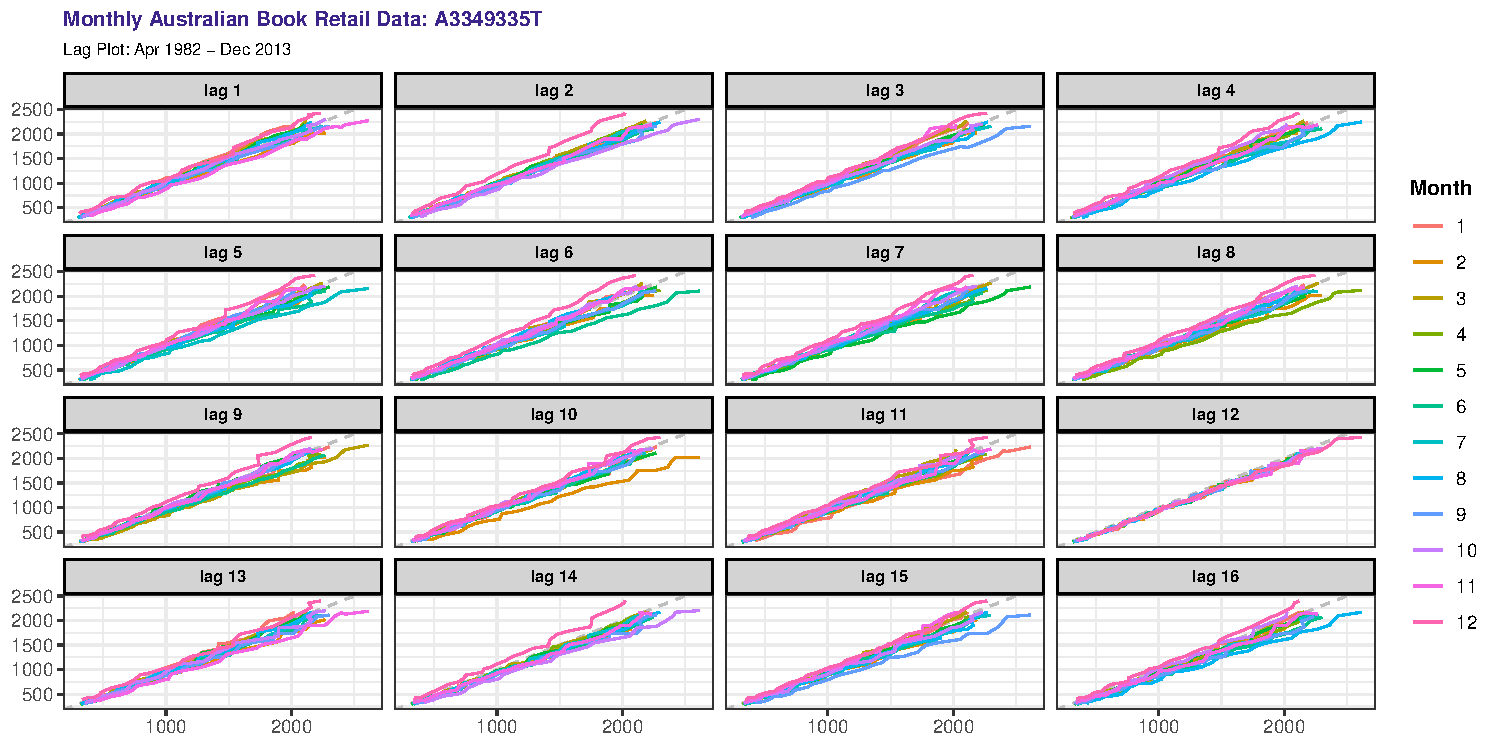
\includegraphics{homework-one_files/figure-latex/ha-2.3c-gglagplot-1.pdf}

Lag plots are used to examine the correlation between the X and Y axis over a fixed period of time with a scatterplot. Per the text, ``each graph shows \(y_{t}\) plotted against \(y_{t} - k\) for different values of \(k\).'' The lag plot below shows an overall positive relationship at each lag, indicating a strong seasonal relationship in the series.

\hypertarget{autocorrelation-plot}{%
\subsubsection{Autocorrelation Plot}\label{autocorrelation-plot}}

\begin{Shaded}
\begin{Highlighting}[]
\KeywordTok{ggAcf}\NormalTok{(myts) }\OperatorTok{+}\StringTok{ }\KeywordTok{labs}\NormalTok{(}\DataTypeTok{title =} \StringTok{"Monthly Australian Book Retail Data: A3349335T"}\NormalTok{, }
  \DataTypeTok{subtitle =} \StringTok{"Correlogram Plot: Apr 1982 - Dec 2013"}\NormalTok{, }\DataTypeTok{x =} \StringTok{"Month"}\NormalTok{, }
  \DataTypeTok{y =} \StringTok{"Sales"}\NormalTok{) }\OperatorTok{+}\StringTok{ }\KeywordTok{theme_bw}\NormalTok{() }\OperatorTok{+}\StringTok{ }\KeywordTok{theme}\NormalTok{()}
\end{Highlighting}
\end{Shaded}

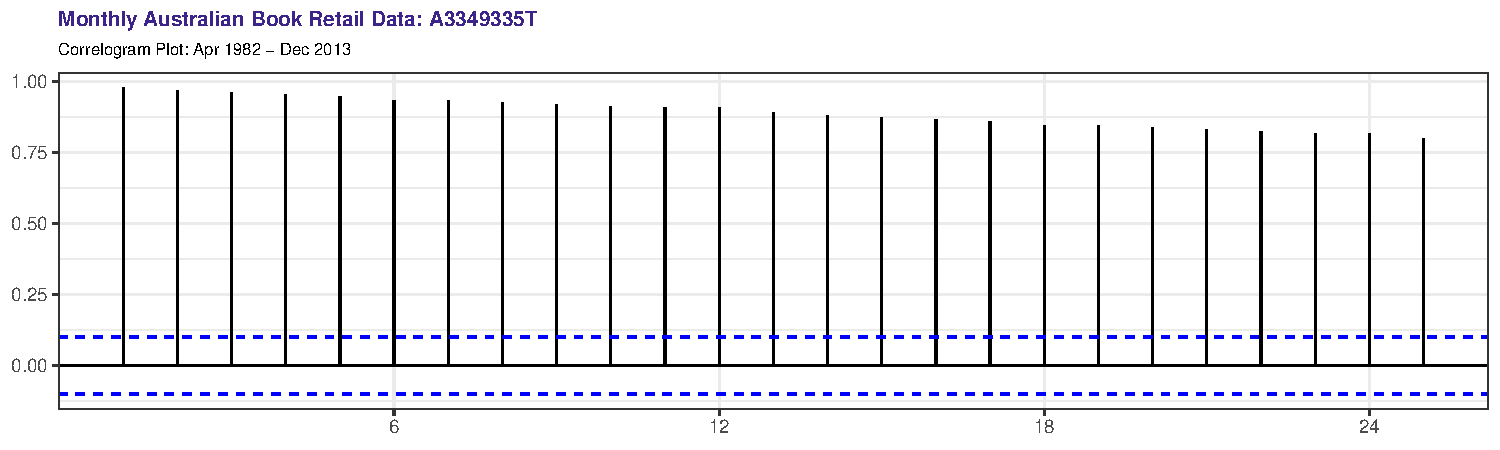
\includegraphics{homework-one_files/figure-latex/ha-2.3c-ggAcf-1.pdf}

Lastly, our autocorrelation plot (also referred to as correlogram plot) measures the linear relationship between the time series' lagged values. Below we used the autocorrelation function \texttt{ggAcf} to examine this relationship for the selected variable from the book retail data. As \(r1\) shows the largest lag and \(r25\) the smallest, this decrease in positive values as lags accrue clearly indicates a trend in the series.

\hypertarget{assignment-two}{%
\chapter{Assignment Two}\label{assignment-two}}

\begin{itemize}
\tightlist
\item
  Hyndman 6.2
\end{itemize}

\hypertarget{hyndman-6.2}{%
\section{Hyndman 6.2}\label{hyndman-6.2}}

\begin{quote}
The \texttt{plastics} dataset consists of the monthly sales (in thousands) of product A for a plastics manufacturer for five years.
\end{quote}

\begin{Shaded}
\begin{Highlighting}[]
\KeywordTok{help}\NormalTok{(plastics)}
\KeywordTok{str}\NormalTok{(plastics)}
\end{Highlighting}
\end{Shaded}

\hypertarget{a.-plot-the-time-series-of-sales-of-product-a.-can-you-identify-seasonal-fluctuations-andor-a-trend-cycle}{%
\subsection{a. Plot the time series of sales of product A. Can you identify seasonal fluctuations and/or a trend-cycle?}\label{a.-plot-the-time-series-of-sales-of-product-a.-can-you-identify-seasonal-fluctuations-andor-a-trend-cycle}}

\begin{Shaded}
\begin{Highlighting}[]
\KeywordTok{autoplot}\NormalTok{(plastics, }\DataTypeTok{main =} \StringTok{"Plastics Product A, Monthly Sales (Five Years)"}\NormalTok{, }
  \DataTypeTok{series =} \StringTok{"Product A"}\NormalTok{, }\DataTypeTok{size =} \FloatTok{0.8}\NormalTok{) }\OperatorTok{+}\StringTok{ }\KeywordTok{autolayer}\NormalTok{(}\KeywordTok{ma}\NormalTok{(plastics, }
  \DataTypeTok{order =} \DecValTok{3}\NormalTok{), }\DataTypeTok{series =} \StringTok{"3-MA"}\NormalTok{, }\DataTypeTok{size =} \FloatTok{0.7}\NormalTok{) }\OperatorTok{+}\StringTok{ }\KeywordTok{autolayer}\NormalTok{(}\KeywordTok{ma}\NormalTok{(plastics, }
  \DataTypeTok{order =} \DecValTok{5}\NormalTok{), }\DataTypeTok{series =} \StringTok{"5-MA"}\NormalTok{, }\DataTypeTok{size =} \FloatTok{0.7}\NormalTok{) }\OperatorTok{+}\StringTok{ }\KeywordTok{autolayer}\NormalTok{(}\KeywordTok{ma}\NormalTok{(plastics, }
  \DataTypeTok{order =} \DecValTok{7}\NormalTok{), }\DataTypeTok{series =} \StringTok{"7-MA"}\NormalTok{, }\DataTypeTok{size =} \FloatTok{0.7}\NormalTok{) }\OperatorTok{+}\StringTok{ }\KeywordTok{autolayer}\NormalTok{(}\KeywordTok{ma}\NormalTok{(plastics, }
  \DataTypeTok{order =} \DecValTok{9}\NormalTok{), }\DataTypeTok{series =} \StringTok{"9-MA"}\NormalTok{, }\DataTypeTok{size =} \FloatTok{0.7}\NormalTok{) }\OperatorTok{+}\StringTok{ }\KeywordTok{autolayer}\NormalTok{(}\KeywordTok{ma}\NormalTok{(plastics, }
  \DataTypeTok{order =} \DecValTok{11}\NormalTok{), }\DataTypeTok{series =} \StringTok{"11-MA"}\NormalTok{, }\DataTypeTok{size =} \FloatTok{0.7}\NormalTok{) }\OperatorTok{+}\StringTok{ }\KeywordTok{autolayer}\NormalTok{(}\KeywordTok{ma}\NormalTok{(plastics, }
  \DataTypeTok{order =} \DecValTok{13}\NormalTok{), }\DataTypeTok{series =} \StringTok{"13-MA"}\NormalTok{, }\DataTypeTok{size =} \FloatTok{0.7}\NormalTok{) }\OperatorTok{+}\StringTok{ }\KeywordTok{ylab}\NormalTok{(}\DataTypeTok{label =} \StringTok{""}\NormalTok{) }\OperatorTok{+}\StringTok{ }
\StringTok{  }\KeywordTok{ylim}\NormalTok{(}\DecValTok{0}\NormalTok{, }\KeywordTok{max}\NormalTok{(plastics)) }\OperatorTok{+}\StringTok{ }\KeywordTok{scale_color_manual}\NormalTok{(}\DataTypeTok{values =} \KeywordTok{c}\NormalTok{(}\StringTok{`}\DataTypeTok{Product A}\StringTok{`}\NormalTok{ =}\StringTok{ "black"}\NormalTok{, }
  \StringTok{`}\DataTypeTok{3-MA}\StringTok{`}\NormalTok{ =}\StringTok{ "red"}\NormalTok{, }\StringTok{`}\DataTypeTok{5-MA}\StringTok{`}\NormalTok{ =}\StringTok{ "rosybrown"}\NormalTok{, }\StringTok{`}\DataTypeTok{7-MA}\StringTok{`}\NormalTok{ =}\StringTok{ "goldenrod3"}\NormalTok{, }
  \StringTok{`}\DataTypeTok{9-MA}\StringTok{`}\NormalTok{ =}\StringTok{ "olivedrab"}\NormalTok{, }\StringTok{`}\DataTypeTok{11-MA}\StringTok{`}\NormalTok{ =}\StringTok{ "royalblue4"}\NormalTok{, }\StringTok{`}\DataTypeTok{13-MA}\StringTok{`}\NormalTok{ =}\StringTok{ "midnightblue"}\NormalTok{), }
  \DataTypeTok{breaks =} \KeywordTok{c}\NormalTok{(}\StringTok{"Product A"}\NormalTok{, }\StringTok{"3-MA"}\NormalTok{, }\StringTok{"5-MA"}\NormalTok{, }\StringTok{"7-MA"}\NormalTok{, }\StringTok{"9-MA"}\NormalTok{, }
    \StringTok{"11-MA"}\NormalTok{, }\StringTok{"13-MA"}\NormalTok{)) }\OperatorTok{+}\StringTok{ }\KeywordTok{theme_bw}\NormalTok{() }\OperatorTok{+}\StringTok{ }\KeywordTok{theme}\NormalTok{()}
\end{Highlighting}
\end{Shaded}

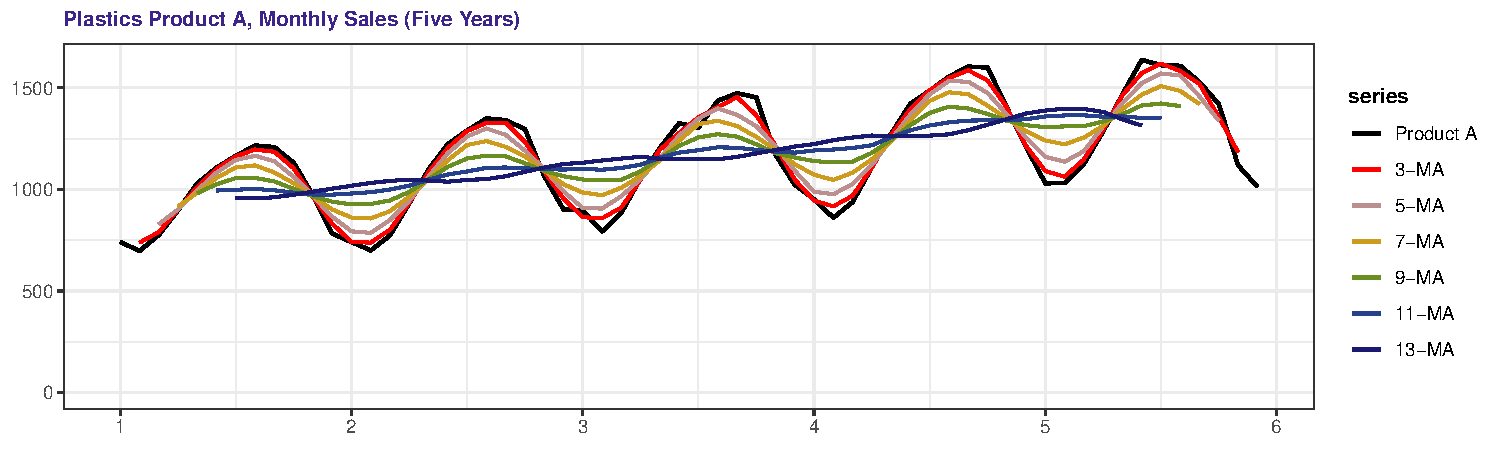
\includegraphics{homework-one_files/figure-latex/ha6.2a-1.pdf}

For this question, we plotted the monthly plastics time series together with moving averages of order 3, 5, 7, 9, 11, and 13. There's a clear seasonal fluctuation, exhibiting troughs at the beginning of each year and peaks over August through October. Additionally, there's a consistent upward trend.

\hypertarget{b.-use-a-classical-multiplicative-decomposition-to-calculate-the-trend-cycle-and-seasonal-indices.}{%
\subsection{b. Use a classical multiplicative decomposition to calculate the trend cycle and seasonal indices.}\label{b.-use-a-classical-multiplicative-decomposition-to-calculate-the-trend-cycle-and-seasonal-indices.}}

\begin{Shaded}
\begin{Highlighting}[]
\CommentTok{# Produce multiplicative decomposition of time series}
\NormalTok{plastics_decomp <-}\StringTok{ }\NormalTok{plastics }\OperatorTok\StringTok{ }\KeywordTok{decompose}\NormalTok{(}\DataTypeTok{type =} \StringTok{"multiplicative"}\NormalTok{)}

\CommentTok{# Plot}
\NormalTok{plastics }\OperatorTok\StringTok{ }\KeywordTok{decompose}\NormalTok{(}\DataTypeTok{type =} \StringTok{"multiplicative"}\NormalTok{) }\OperatorTok\StringTok{ }\KeywordTok{autoplot}\NormalTok{() }\OperatorTok{+}\StringTok{ }
\StringTok{  }\KeywordTok{xlab}\NormalTok{(}\StringTok{"Month"}\NormalTok{) }\OperatorTok{+}\StringTok{ }\KeywordTok{ylab}\NormalTok{(}\StringTok{"Sales"}\NormalTok{) }\OperatorTok{+}\StringTok{ }\KeywordTok{theme_bw}\NormalTok{() }\OperatorTok{+}\StringTok{ }\KeywordTok{theme}\NormalTok{()}
\end{Highlighting}
\end{Shaded}

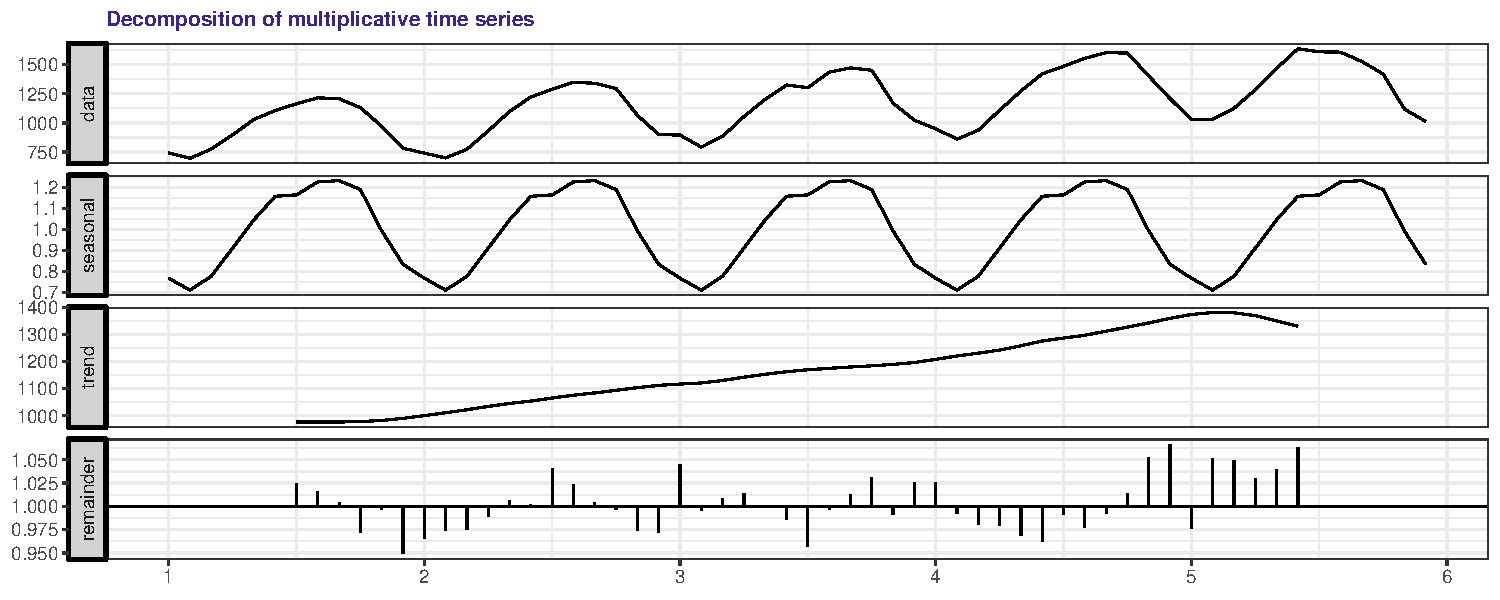
\includegraphics{homework-one_files/figure-latex/ha6.2b-1.pdf}

\begin{Shaded}
\begin{Highlighting}[]
\CommentTok{# Output the trend strength and seasonal strength metrics}
\NormalTok{plastics }\OperatorTok\StringTok{ }\KeywordTok{tsfeatures}\NormalTok{() }\OperatorTok\StringTok{ }\KeywordTok{select}\NormalTok{(trend, seasonal_strength) }\OperatorTok\StringTok{ }
\StringTok{  }\KeywordTok{rename}\NormalTok{(}\DataTypeTok{trend_str =}\NormalTok{ trend, }\DataTypeTok{season_str =}\NormalTok{ seasonal_strength)}
\end{Highlighting}
\end{Shaded}

\begin{verbatim}
FALSE # A tibble: 1 x 2
FALSE   trend_str season_str
FALSE       <dbl>      <dbl>
FALSE 1     0.919      0.964
\end{verbatim}

\begin{Shaded}
\begin{Highlighting}[]
\CommentTok{# The tsfeatures package provides statistics on strength}
\CommentTok{# of trend and seasonality, which doesn't seem to be a}
\CommentTok{# built-in feature of the forecast or other time series}
\CommentTok{# packages:}
\CommentTok{# https://rdrr.io/github/robjhyndman/tsfeatures/man/stl_features.html}

\CommentTok{# Output the seasonal index}
\NormalTok{(}\ControlFlowTok{function}\NormalTok{(x) }\KeywordTok{print}\NormalTok{(}\KeywordTok{paste}\NormalTok{(}\KeywordTok{min}\NormalTok{(x), }\KeywordTok{max}\NormalTok{(x))))(plastics_decomp}\OperatorTok{$}\NormalTok{figure)}
\end{Highlighting}
\end{Shaded}

\begin{verbatim}
FALSE [1] "0.710335708434527 1.23136353496152"
\end{verbatim}

The multiplicative decomposition, with \(F_S\) of .963 (close to the maximum of 1), substantiates the strong seasonal trend observed in the data. The seaonsal index ranges between .71 and 1.23. The trend is also strong, with \(F_T\) of .92 (also close to the maximum of 1), which supports our answer for \(c.\).

\hypertarget{c.-do-the-results-support-the-graphical-interpretations-from-part-a}{%
\subsection{c. Do the results support the graphical interpretations from part a?}\label{c.-do-the-results-support-the-graphical-interpretations-from-part-a}}

Yes, when decomposed, the trend becomes very clearly upward, while a rather unvarying seasonal component emerges. The one very interesting component is the random, component, it does seem to imply an unexpained mechanism (with some variability over time).

\hypertarget{d.-compute-and-plot-the-seasonally-adjusted-data.}{%
\subsection{d. Compute and plot the seasonally adjusted data.}\label{d.-compute-and-plot-the-seasonally-adjusted-data.}}

\begin{Shaded}
\begin{Highlighting}[]
\CommentTok{# Compute the seasonally adjusted monthly plastics time}
\CommentTok{# series}
\NormalTok{plastics_seasadj <-}\StringTok{ }\NormalTok{plastics}\OperatorTok{/}\NormalTok{plastics_decomp}\OperatorTok{$}\NormalTok{seasonal}

\CommentTok{# Plot the seasonally adjusted monthly plastics time}
\CommentTok{# series}
\KeywordTok{autoplot}\NormalTok{(plastics_seasadj, }\DataTypeTok{main =} \StringTok{"Plastics Product A, Seasonally Adjusted Monthly Sales (Five Years)"}\NormalTok{, }
  \DataTypeTok{series =} \StringTok{"Product A (Seasonally Adjusted)"}\NormalTok{, }\DataTypeTok{size =} \FloatTok{0.7}\NormalTok{, }
  \DataTypeTok{color =} \StringTok{"black"}\NormalTok{) }\OperatorTok{+}\StringTok{ }\KeywordTok{theme_bw}\NormalTok{() }\OperatorTok{+}\StringTok{ }\KeywordTok{theme}\NormalTok{() }\OperatorTok{+}\StringTok{ }\KeywordTok{ylab}\NormalTok{(}\DataTypeTok{label =} \StringTok{""}\NormalTok{) }\OperatorTok{+}\StringTok{ }
\StringTok{  }\KeywordTok{ylim}\NormalTok{(}\DecValTok{0}\NormalTok{, }\KeywordTok{max}\NormalTok{(plastics_seasadj))}
\end{Highlighting}
\end{Shaded}

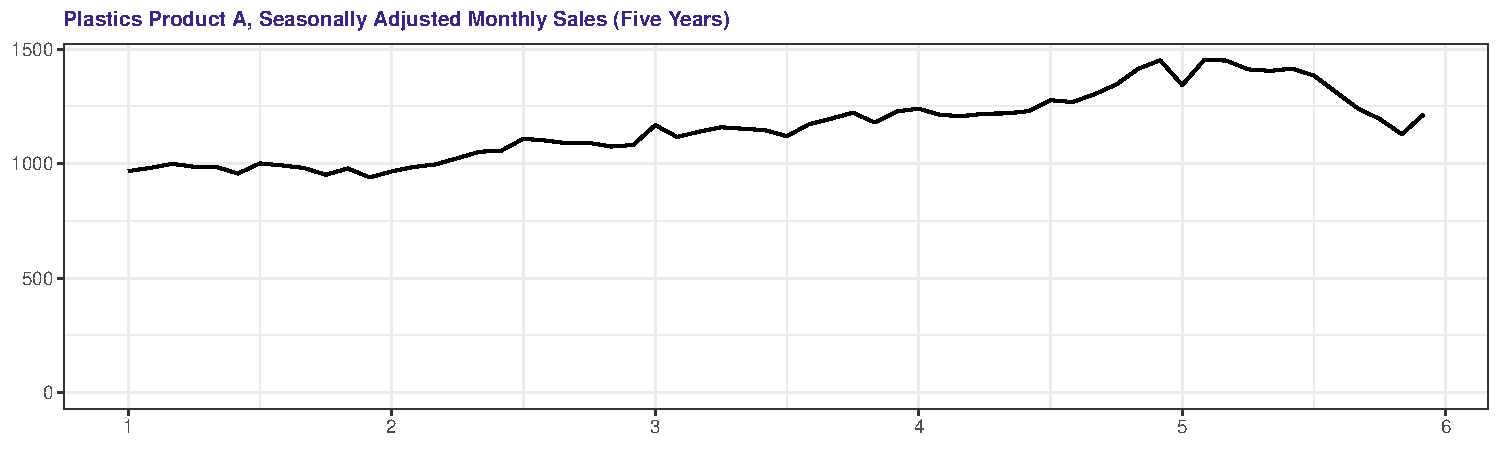
\includegraphics{homework-one_files/figure-latex/ha6.2d-1.pdf}

\hypertarget{e.-change-one-observation-to-be-an-outlier-and-recompute-the-seasonally-adjusted-data.-what-is-the-effect-of-the-outlier}{%
\subsection{e. Change one observation to be an outlier and recompute the seasonally adjusted data. What is the effect of the outlier?}\label{e.-change-one-observation-to-be-an-outlier-and-recompute-the-seasonally-adjusted-data.-what-is-the-effect-of-the-outlier}}

\begin{Shaded}
\begin{Highlighting}[]
\CommentTok{# Artifically change single observation to create outlier}
\CommentTok{# between 1.5x IQR in middle of time series}
\NormalTok{plastics_}\DecValTok{2}\NormalTok{ <-}\StringTok{ }\NormalTok{plastics}
\NormalTok{plastics_}\DecValTok{2}\NormalTok{[}\DecValTok{25}\NormalTok{] <-}\StringTok{ }\KeywordTok{quantile}\NormalTok{(plastics_}\DecValTok{2}\NormalTok{)[}\DecValTok{4}\NormalTok{] }\OperatorTok{*}\StringTok{ }\FloatTok{1.5}
\NormalTok{plastics_}\DecValTok{2}\NormalTok{_decomp <-}\StringTok{ }\KeywordTok{decompose}\NormalTok{(plastics_}\DecValTok{2}\NormalTok{, }\DataTypeTok{type =} \StringTok{"multiplicative"}\NormalTok{)}
\NormalTok{plastics_}\DecValTok{2}\NormalTok{_seasadj <-}\StringTok{ }\NormalTok{plastics_}\DecValTok{2}\OperatorTok{/}\NormalTok{plastics_}\DecValTok{2}\NormalTok{_decomp}\OperatorTok{$}\NormalTok{seasonal}

\CommentTok{# Plot the seasonally adjusted monthly plastics time}
\CommentTok{# series}
\KeywordTok{autoplot}\NormalTok{(plastics_}\DecValTok{2}\NormalTok{_seasadj, }\DataTypeTok{main =} \StringTok{"Plastics Product A, Seasonally Adjusted Monthly Sales With Artificial Outlier (Five Years)"}\NormalTok{, }
  \DataTypeTok{series =} \StringTok{"Product A (Seasonally Adjusted)"}\NormalTok{, }\DataTypeTok{size =} \FloatTok{0.7}\NormalTok{, }
  \DataTypeTok{color =} \StringTok{"black"}\NormalTok{) }\OperatorTok{+}\StringTok{ }\KeywordTok{theme_bw}\NormalTok{() }\OperatorTok{+}\StringTok{ }\KeywordTok{theme}\NormalTok{() }\OperatorTok{+}\StringTok{ }\KeywordTok{ylab}\NormalTok{(}\DataTypeTok{label =} \StringTok{""}\NormalTok{) }\OperatorTok{+}\StringTok{ }
\StringTok{  }\KeywordTok{ylim}\NormalTok{(}\DecValTok{0}\NormalTok{, }\KeywordTok{max}\NormalTok{(plastics_}\DecValTok{2}\NormalTok{_seasadj))}
\end{Highlighting}
\end{Shaded}

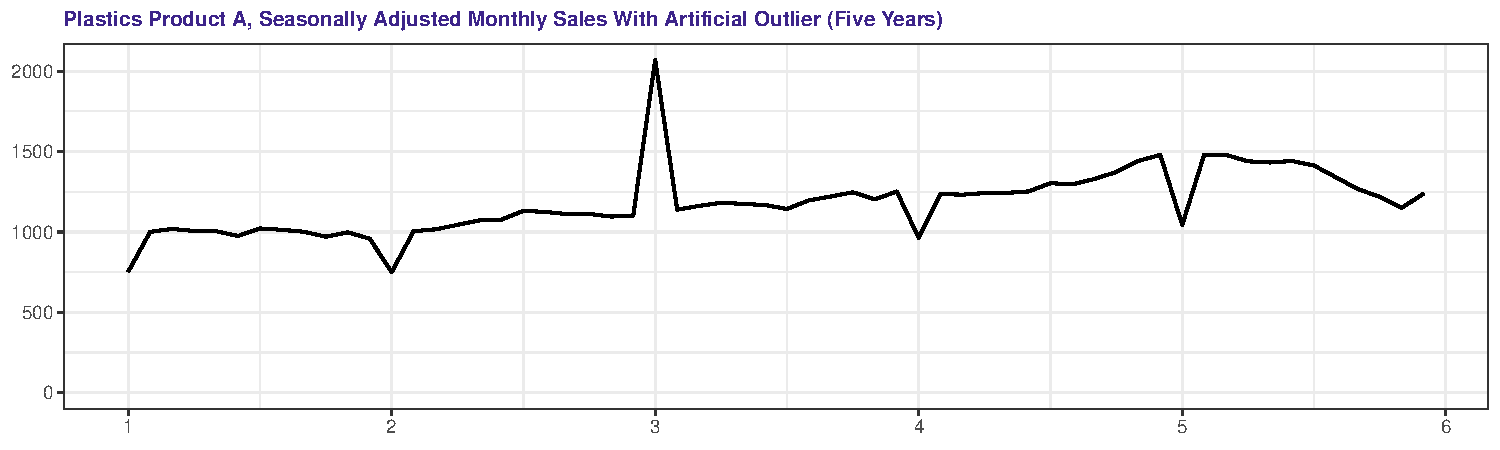
\includegraphics{homework-one_files/figure-latex/ha6.2e-1.pdf}

The effect is to deflate the corresponding month in other years in the seasonally adjusted data. In this case, the first month (January) of Year 3 was artifically inflated to approximately 2,111, which is 1.5 times larger than the upper bound of the inter-quartile range (the minimum value for an outlier). The second months of years 1-2 and 4-5 have all fallen to compensate together for this outlier and now represent troughs.

\hypertarget{f.-does-it-make-any-difference-if-the-outlier-is-near-the-end-rather-than-in-the-middle-of-the-time-series}{%
\subsection{f. Does it make any difference if the outlier is near the end rather than in the middle of the time series?}\label{f.-does-it-make-any-difference-if-the-outlier-is-near-the-end-rather-than-in-the-middle-of-the-time-series}}

\begin{Shaded}
\begin{Highlighting}[]
\CommentTok{# Create outliers at beginning and end of respective time}
\CommentTok{# series}
\NormalTok{plastics_}\DecValTok{3}\NormalTok{ <-}\StringTok{ }\NormalTok{plastics}
\NormalTok{plastics_}\DecValTok{3}\NormalTok{[}\DecValTok{46}\NormalTok{] <-}\StringTok{ }\KeywordTok{quantile}\NormalTok{(plastics_}\DecValTok{3}\NormalTok{)[}\DecValTok{4}\NormalTok{] }\OperatorTok{*}\StringTok{ }\FloatTok{1.5}
\NormalTok{plastics_}\DecValTok{3}\NormalTok{_decomp <-}\StringTok{ }\KeywordTok{decompose}\NormalTok{(plastics_}\DecValTok{3}\NormalTok{, }\DataTypeTok{type =} \StringTok{"multiplicative"}\NormalTok{)}
\NormalTok{plastics_}\DecValTok{3}\NormalTok{_seasadj <-}\StringTok{ }\NormalTok{plastics_}\DecValTok{3}\OperatorTok{/}\NormalTok{plastics_}\DecValTok{3}\NormalTok{_decomp}\OperatorTok{$}\NormalTok{seasonal}

\NormalTok{plastics_}\DecValTok{4}\NormalTok{ <-}\StringTok{ }\NormalTok{plastics}
\NormalTok{plastics_}\DecValTok{4}\NormalTok{[}\DecValTok{3}\NormalTok{] <-}\StringTok{ }\KeywordTok{quantile}\NormalTok{(plastics_}\DecValTok{4}\NormalTok{)[}\DecValTok{4}\NormalTok{] }\OperatorTok{*}\StringTok{ }\FloatTok{1.5}
\NormalTok{plastics_}\DecValTok{4}\NormalTok{_decomp <-}\StringTok{ }\KeywordTok{decompose}\NormalTok{(plastics_}\DecValTok{4}\NormalTok{, }\DataTypeTok{type =} \StringTok{"multiplicative"}\NormalTok{)}
\NormalTok{plastics_}\DecValTok{4}\NormalTok{_seasadj <-}\StringTok{ }\NormalTok{plastics_}\DecValTok{4}\OperatorTok{/}\NormalTok{plastics_}\DecValTok{4}\NormalTok{_decomp}\OperatorTok{$}\NormalTok{seasonal}

\CommentTok{# autoplot(plastics_4_seasadj)}

\CommentTok{# Plot different outlier time series for comparison}
\KeywordTok{autoplot}\NormalTok{(plastics_}\DecValTok{2}\NormalTok{_seasadj, }\DataTypeTok{main =} \StringTok{"Plastics Product A, Seasonally Adjusted Monthly Sales (Five Years)"}\NormalTok{, }
  \DataTypeTok{series =} \StringTok{"SeasAdj w/ Outlier: Yr3 Jan"}\NormalTok{, }\DataTypeTok{size =} \FloatTok{0.75}\NormalTok{) }\OperatorTok{+}\StringTok{ }
\StringTok{  }\KeywordTok{autolayer}\NormalTok{(plastics_}\DecValTok{3}\NormalTok{_seasadj, }\DataTypeTok{series =} \StringTok{"SeasAdj w/ Outlier: Yr5 Aug"}\NormalTok{, }
    \DataTypeTok{size =} \FloatTok{0.75}\NormalTok{) }\OperatorTok{+}\StringTok{ }\KeywordTok{autolayer}\NormalTok{(plastics_}\DecValTok{4}\NormalTok{_seasadj, }\DataTypeTok{series =} \StringTok{"SeasAdj w/ Outlier: Yr1 Mar"}\NormalTok{, }
  \DataTypeTok{size =} \FloatTok{0.75}\NormalTok{) }\OperatorTok{+}\StringTok{ }\KeywordTok{theme_bw}\NormalTok{() }\OperatorTok{+}\StringTok{ }\KeywordTok{theme}\NormalTok{() }\OperatorTok{+}\StringTok{ }\KeywordTok{ylab}\NormalTok{(}\DataTypeTok{label =} \StringTok{""}\NormalTok{) }\OperatorTok{+}\StringTok{ }
\StringTok{  }\KeywordTok{ylim}\NormalTok{(}\DecValTok{0}\NormalTok{, }\KeywordTok{max}\NormalTok{(}\KeywordTok{c}\NormalTok{(}\KeywordTok{max}\NormalTok{(plastics_seasadj), }\KeywordTok{max}\NormalTok{(plastics_}\DecValTok{2}\NormalTok{_seasadj), }
    \KeywordTok{max}\NormalTok{(plastics_}\DecValTok{3}\NormalTok{_seasadj), }\KeywordTok{max}\NormalTok{(plastics_}\DecValTok{4}\NormalTok{_seasadj)))) }\OperatorTok{+}\StringTok{ }
\StringTok{  }\KeywordTok{scale_color_manual}\NormalTok{(}\DataTypeTok{values =} \KeywordTok{c}\NormalTok{(}\DataTypeTok{SeasAdj =} \StringTok{"black"}\NormalTok{, }\StringTok{`}\DataTypeTok{SeasAdj w/ Outlier: Yr1 Mar}\StringTok{`}\NormalTok{ =}\StringTok{ "red"}\NormalTok{, }
    \StringTok{`}\DataTypeTok{SeasAdj w/ Outlier: Yr3 Jan}\StringTok{`}\NormalTok{ =}\StringTok{ "goldenrod3"}\NormalTok{, }\StringTok{`}\DataTypeTok{SeasAdj w/ Outlier: Yr5 Aug}\StringTok{`}\NormalTok{ =}\StringTok{ "royalblue4"}\NormalTok{), }
    \DataTypeTok{breaks =} \KeywordTok{c}\NormalTok{(}\StringTok{"SeasAdj"}\NormalTok{, }\StringTok{"SeasAdj w/ Outlier: Yr1 Mar"}\NormalTok{, }
      \StringTok{"SeasAdj w/ Outlier: Yr3 Jan"}\NormalTok{, }\StringTok{"SeasAdj w/ Outlier: Yr5 Aug"}\NormalTok{))}
\end{Highlighting}
\end{Shaded}

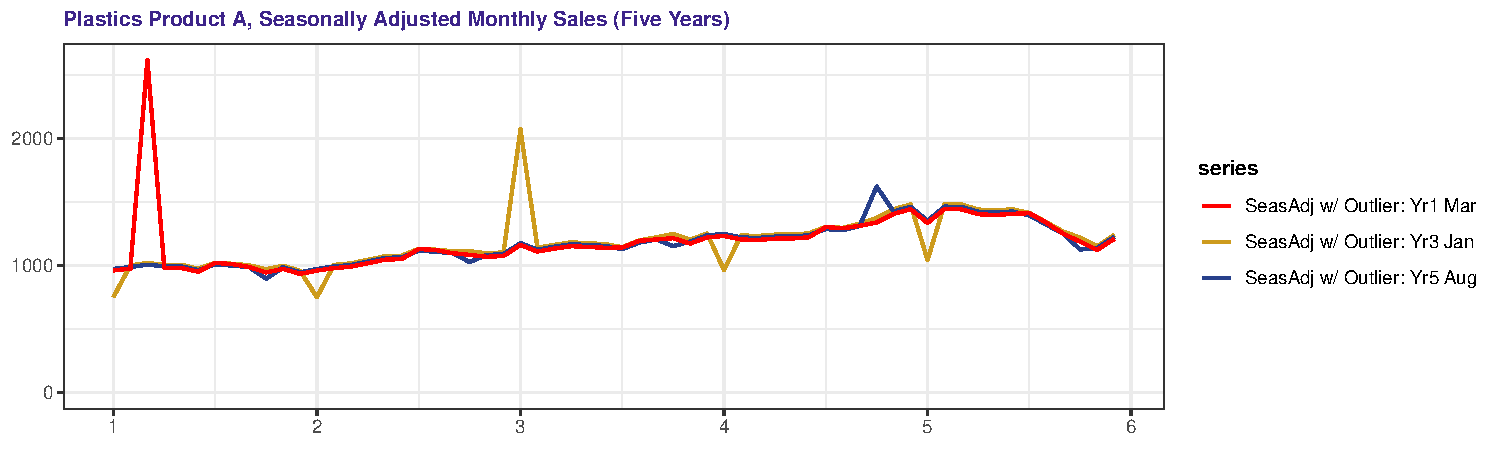
\includegraphics{homework-one_files/figure-latex/ha6.2f-1.pdf}

\hypertarget{assignment-three}{%
\chapter{Assignment Three}\label{assignment-three}}

\begin{itemize}
\tightlist
\item
  Kuhn \& Johnson 3.1\\
\item
  Kuhn \& Johnson 3.2
\end{itemize}

\hypertarget{kuhn-johnson-3.1}{%
\section{Kuhn \& Johnson 3.1}\label{kuhn-johnson-3.1}}

\begin{quote}
The UC Irvine Machine Learning Repository contains a data set related to glass identification. The data consist of 214 glass samples labeled as one of seven class categories. There are nine predictors, including the refractive index and percentages of eight elements: Na, Mg, Al, Si, K, Ca, Ba, and Fe.
\end{quote}

\hypertarget{a.-using-visualizations-explore-the-predictor-variables-to-understand-their-distributions-as-well-as-the-relationships-between-predictors.}{%
\subsection{a. Using visualizations, explore the predictor variables to understand their distributions as well as the relationships between predictors.}\label{a.-using-visualizations-explore-the-predictor-variables-to-understand-their-distributions-as-well-as-the-relationships-between-predictors.}}

\hypertarget{descriptive-statistics}{%
\subsubsection{Descriptive Statistics}\label{descriptive-statistics}}

The output of the \texttt{describe(\ )} function suggests some variables to take closer looks at. RI, Mg, K, Ca, Ba and Fe appear skewed; and RI, Na, Si, K , Ca, Ba, and (to a lesser extent) Fe exhibit some challenging tails (kurtosis != 3.0).

\begin{table}[!h]

\caption{\label{tab:glass-basics}Summary Statistics of Glass data}
\centering
\fontsize{10}{12}\selectfont
\begin{tabu} to \linewidth {>{\raggedright}X>{\raggedleft}X>{\raggedleft}X>{\raggedleft}X>{\raggedleft}X>{\raggedleft}X>{\raggedleft}X>{\raggedleft}X>{\raggedleft}X>{\raggedleft}X>{\raggedleft}X>{\raggedleft}X>{\raggedleft}X>{\raggedleft}X}
\hline
  & vars & n & mean & sd & median & trimmed & mad & min & max & range & skew & kurtosis & se\\
\hline
\rowcolor{gray!6}  RI & 1 & 214 & 1.52 & 0.00 & 1.52 & 1.52 & 0.00 & 1.51 & 1.53 & 0.02 & 1.60 & 4.72 & 0.00\\
\hline
Na & 2 & 214 & 13.41 & 0.82 & 13.30 & 13.38 & 0.64 & 10.73 & 17.38 & 6.65 & 0.45 & 2.90 & 0.06\\
\hline
\rowcolor{gray!6}  Mg & 3 & 214 & 2.68 & 1.44 & 3.48 & 2.87 & 0.30 & 0.00 & 4.49 & 4.49 & -1.14 & -0.45 & 0.10\\
\hline
Al & 4 & 214 & 1.44 & 0.50 & 1.36 & 1.41 & 0.31 & 0.29 & 3.50 & 3.21 & 0.89 & 1.94 & 0.03\\
\hline
\rowcolor{gray!6}  Si & 5 & 214 & 72.65 & 0.77 & 72.79 & 72.71 & 0.57 & 69.81 & 75.41 & 5.60 & -0.72 & 2.82 & 0.05\\
\hline
K & 6 & 214 & 0.50 & 0.65 & 0.56 & 0.43 & 0.17 & 0.00 & 6.21 & 6.21 & 6.46 & 52.87 & 0.04\\
\hline
\rowcolor{gray!6}  Ca & 7 & 214 & 8.96 & 1.42 & 8.60 & 8.74 & 0.66 & 5.43 & 16.19 & 10.76 & 2.02 & 6.41 & 0.10\\
\hline
Ba & 8 & 214 & 0.18 & 0.50 & 0.00 & 0.03 & 0.00 & 0.00 & 3.15 & 3.15 & 3.37 & 12.08 & 0.03\\
\hline
\rowcolor{gray!6}  Fe & 9 & 214 & 0.06 & 0.10 & 0.00 & 0.04 & 0.00 & 0.00 & 0.51 & 0.51 & 1.73 & 2.52 & 0.01\\
\hline
Type* & 10 & 214 & 2.54 & 1.71 & 2.00 & 2.31 & 1.48 & 1.00 & 6.00 & 5.00 & 1.04 & -0.29 & 0.12\\
\hline
\end{tabu}
\end{table}

\hypertarget{skewness}{%
\subsubsection{Skewness}\label{skewness}}

We can also look at the skew of our numeric variables using the \texttt{e1071} package:

\begin{Shaded}
\begin{Highlighting}[]
\NormalTok{skewer<-}\ControlFlowTok{function}\NormalTok{(df)\{}
\NormalTok{  new_skew =}\StringTok{ }\KeywordTok{setNames}\NormalTok{(}\KeywordTok{data.frame}\NormalTok{(}\KeywordTok{matrix}\NormalTok{(}\DataTypeTok{ncol =} \DecValTok{2}\NormalTok{, }\DataTypeTok{nrow =} \DecValTok{0}\NormalTok{)), }\KeywordTok{c}\NormalTok{(}\StringTok{"Element"}\NormalTok{, }\StringTok{"Skew"}\NormalTok{))}
    \ControlFlowTok{for}\NormalTok{(name }\ControlFlowTok{in} \KeywordTok{colnames}\NormalTok{(df))\{}
\NormalTok{    skew <-}\KeywordTok{skewness}\NormalTok{(df[,name])}
\NormalTok{    temp =}\StringTok{ }\KeywordTok{data.frame}\NormalTok{(}\KeywordTok{cbind}\NormalTok{(}\StringTok{'Element'}\NormalTok{ =name, }\StringTok{'Skew'}\NormalTok{ =skew))}
\NormalTok{    new_skew <-}\KeywordTok{rbind}\NormalTok{(new_skew, temp)\}}
  \KeywordTok{return}\NormalTok{(new_skew)}
\NormalTok{\}}

\KeywordTok{skewer}\NormalTok{(Glass[, }\DecValTok{1}\OperatorTok{:}\DecValTok{9}\NormalTok{])}\OperatorTok
\StringTok{  }\KeywordTok{kable}\NormalTok{(}\StringTok{"latex"}\NormalTok{) }\OperatorTok
\StringTok{  }\KeywordTok{kable_styling}\NormalTok{(}\DataTypeTok{latex_options =} \KeywordTok{c}\NormalTok{(}\StringTok{"hold_position"}\NormalTok{, }\StringTok{"striped"}\NormalTok{))}
\end{Highlighting}
\end{Shaded}

\begingroup\fontsize{10}{12}\selectfont

\begin{tabu} to \linewidth {>{\raggedright}X>{\raggedright}X}
\hline
Element & Skew\\
\hline
\rowcolor{gray!6}  RI & 1.60271508274373\\
\hline
Na & 0.447834258917133\\
\hline
\rowcolor{gray!6}  Mg & -1.13645227846653\\
\hline
Al & 0.89461041611312\\
\hline
\rowcolor{gray!6}  Si & -0.720239210805621\\
\hline
K & 6.46008889572281\\
\hline
\rowcolor{gray!6}  Ca & 2.01844629445302\\
\hline
Ba & 3.36867996880571\\
\hline
\rowcolor{gray!6}  Fe & 1.7298107095598\\
\hline
\end{tabu}
\endgroup{}

\hypertarget{distribution}{%
\subsubsection{Distribution}\label{distribution}}

Histograms visually illustrate the challenges with these distributions.

\begin{Shaded}
\begin{Highlighting}[]
\NormalTok{Glass }\OperatorTok\StringTok{ }\KeywordTok{keep}\NormalTok{(is.numeric) }\OperatorTok\StringTok{ }\KeywordTok{gather}\NormalTok{() }\OperatorTok\StringTok{ }\KeywordTok{ggplot}\NormalTok{(}\KeywordTok{aes}\NormalTok{(value)) }\OperatorTok{+}\StringTok{ }
\StringTok{  }\KeywordTok{facet_wrap}\NormalTok{(}\OperatorTok{~}\NormalTok{key, }\DataTypeTok{scales =} \StringTok{"free"}\NormalTok{) }\OperatorTok{+}\StringTok{ }\KeywordTok{geom_histogram}\NormalTok{(}\DataTypeTok{fill =} \StringTok{"darkorchid"}\NormalTok{, }
  \DataTypeTok{color =} \StringTok{"black"}\NormalTok{) }\OperatorTok{+}\StringTok{ }\KeywordTok{theme_bw}\NormalTok{()}
\end{Highlighting}
\end{Shaded}

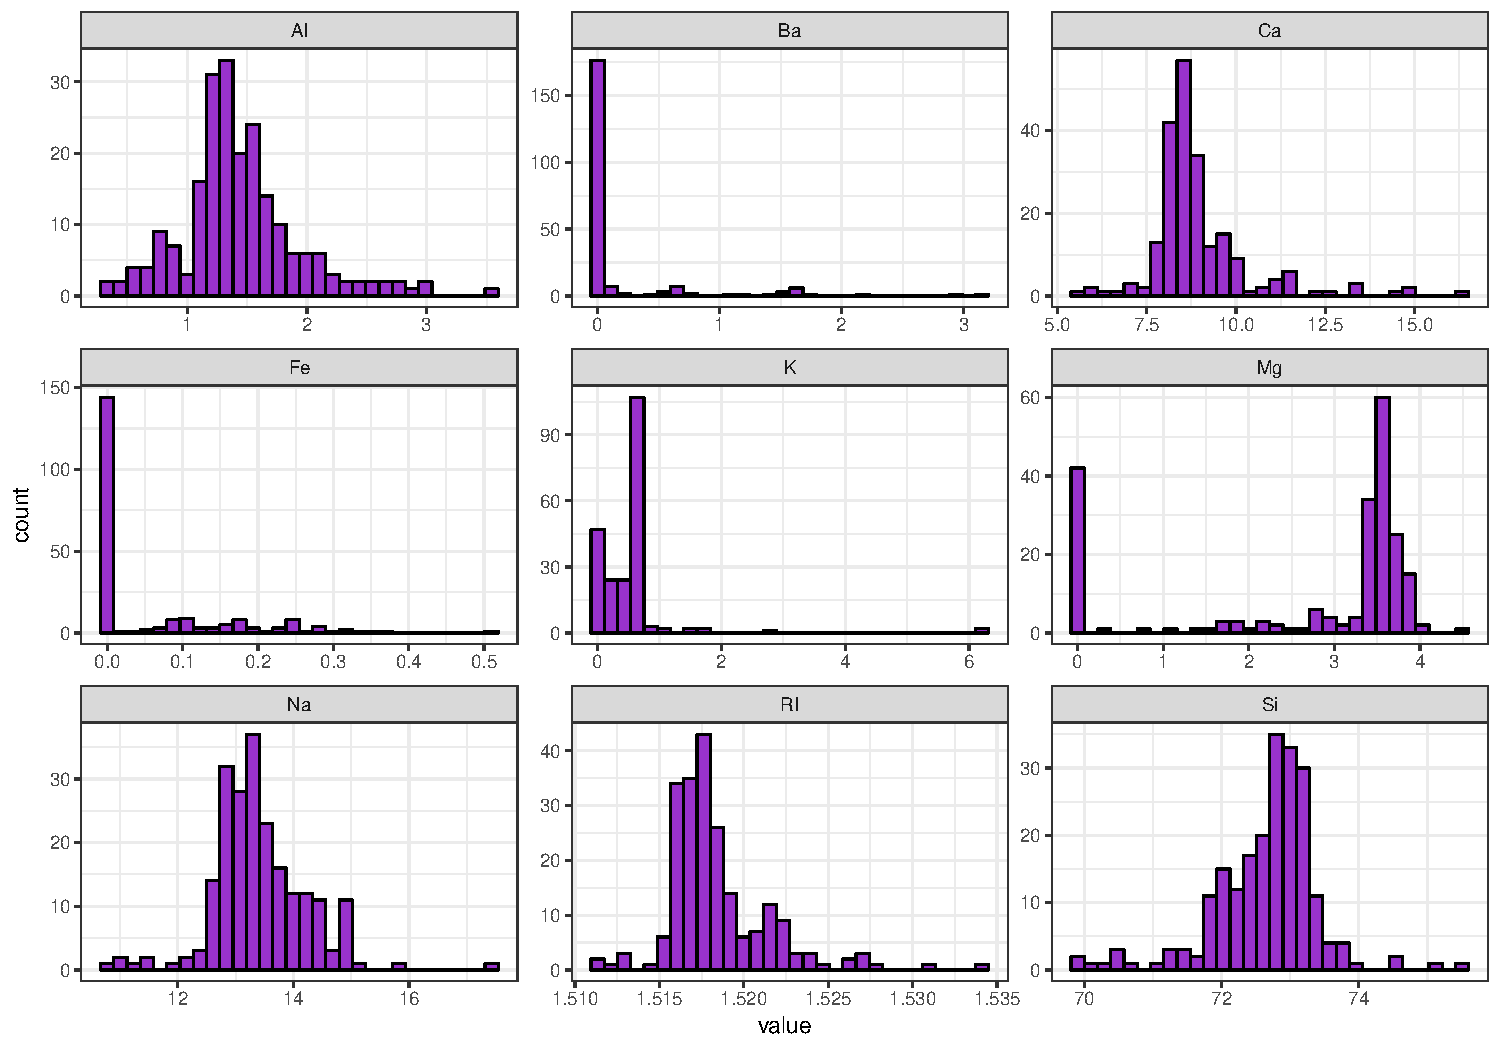
\includegraphics{homework-one_files/figure-latex/glass-1.pdf}

\hypertarget{correlation}{%
\subsubsection{Correlation}\label{correlation}}

We used a corrplot to look at the correleations between numeric glass variables.

There is some significant positive correlation between \texttt{Ca} and \texttt{RI}; slightly less between \texttt{Ba} and \texttt{Al}, \texttt{Ba} and \texttt{Na}, and \texttt{K} and \texttt{Al}.

There are some obvious negative correlations between Si and RI, as well as \texttt{Al} and \texttt{RI}, \texttt{Al} and \texttt{Mg}, \texttt{Ca} and \texttt{Mg}, and \texttt{Ba} and \texttt{Mg}.

\begin{Shaded}
\begin{Highlighting}[]
\NormalTok{glassCor <-}\StringTok{ }\KeywordTok{cor}\NormalTok{(Glass[}\OperatorTok{-}\DecValTok{10}\NormalTok{])}
\KeywordTok{corrplot}\NormalTok{(glassCor, }\DataTypeTok{method =} \StringTok{"square"}\NormalTok{, }\DataTypeTok{type =} \StringTok{"lower"}\NormalTok{)}
\end{Highlighting}
\end{Shaded}


\includegraphics{homework-one_files/figure-latex/glass.2-1.pdf}

\hypertarget{b.-do-there-appear-to-be-any-outliers-in-the-data-are-any-predictors-skewed}{%
\subsection{b. Do there appear to be any outliers in the data? Are any predictors skewed?}\label{b.-do-there-appear-to-be-any-outliers-in-the-data-are-any-predictors-skewed}}

\hypertarget{boxplot}{%
\subsubsection{Boxplot}\label{boxplot}}

The long tails of some of the predictors visible in histograms are indicative of outliers. The plot below shows a boxplot and violin plot for each variable. Many of the variables appear to have outliers; \texttt{Ba}, \texttt{Fe} and \texttt{K} appear to have the most potential outliers. Handling these outliers will depend on a mix of reference data and statistical techniques.

Skewness is also visible in the histograms, \texttt{Mg} is bimodal. \texttt{Ba}, \texttt{K} and \texttt{Fe} are right skewed. The remaining variables don't appear to be normally distributed - though they exhibit central tendency, there are signs that they are leptokurtic or platykurtic. This suggests exploring skew and possibly transformations might be of use down the line.

\begin{Shaded}
\begin{Highlighting}[]
\CommentTok{# boxplot with violin plot overlaid for all variables}
\NormalTok{Glass }\OperatorTok\StringTok{ }\KeywordTok{keep}\NormalTok{(is.numeric) }\OperatorTok\StringTok{ }\KeywordTok{gather}\NormalTok{() }\OperatorTok\StringTok{ }\KeywordTok{group_by}\NormalTok{(key) }\OperatorTok\StringTok{ }
\StringTok{  }\KeywordTok{ggplot}\NormalTok{(}\DataTypeTok{data =}\NormalTok{ ., }\KeywordTok{aes}\NormalTok{(}\DataTypeTok{x =} \StringTok{""}\NormalTok{, }\DataTypeTok{y =}\NormalTok{ value)) }\OperatorTok{+}\StringTok{ }\KeywordTok{geom_boxplot}\NormalTok{() }\OperatorTok{+}\StringTok{ }
\StringTok{  }\KeywordTok{geom_boxplot}\NormalTok{(}\DataTypeTok{outlier.colour =} \StringTok{"orange"}\NormalTok{, }\DataTypeTok{fill =} \StringTok{"grey"}\NormalTok{) }\OperatorTok{+}\StringTok{ }
\StringTok{  }\KeywordTok{geom_violin}\NormalTok{(}\DataTypeTok{alpha =} \FloatTok{0.3}\NormalTok{, }\DataTypeTok{color =} \OtherTok{NA}\NormalTok{, }\DataTypeTok{fill =} \StringTok{"lightblue"}\NormalTok{) }\OperatorTok{+}\StringTok{ }
\StringTok{  }\KeywordTok{labs}\NormalTok{(}\DataTypeTok{x =} \OtherTok{NULL}\NormalTok{, }\DataTypeTok{y =} \OtherTok{NULL}\NormalTok{) }\OperatorTok{+}\StringTok{ }\KeywordTok{theme_bw}\NormalTok{() }\OperatorTok{+}\StringTok{ }\KeywordTok{theme}\NormalTok{(}\DataTypeTok{axis.ticks.y =} \KeywordTok{element_blank}\NormalTok{()) }\OperatorTok{+}\StringTok{ }
\StringTok{  }\KeywordTok{facet_wrap}\NormalTok{(}\OperatorTok{~}\NormalTok{key, }\DataTypeTok{scales =} \StringTok{"free"}\NormalTok{, }\DataTypeTok{ncol =} \DecValTok{3}\NormalTok{) }\OperatorTok{+}\StringTok{ }\KeywordTok{coord_flip}\NormalTok{()}
\end{Highlighting}
\end{Shaded}

\begin{center}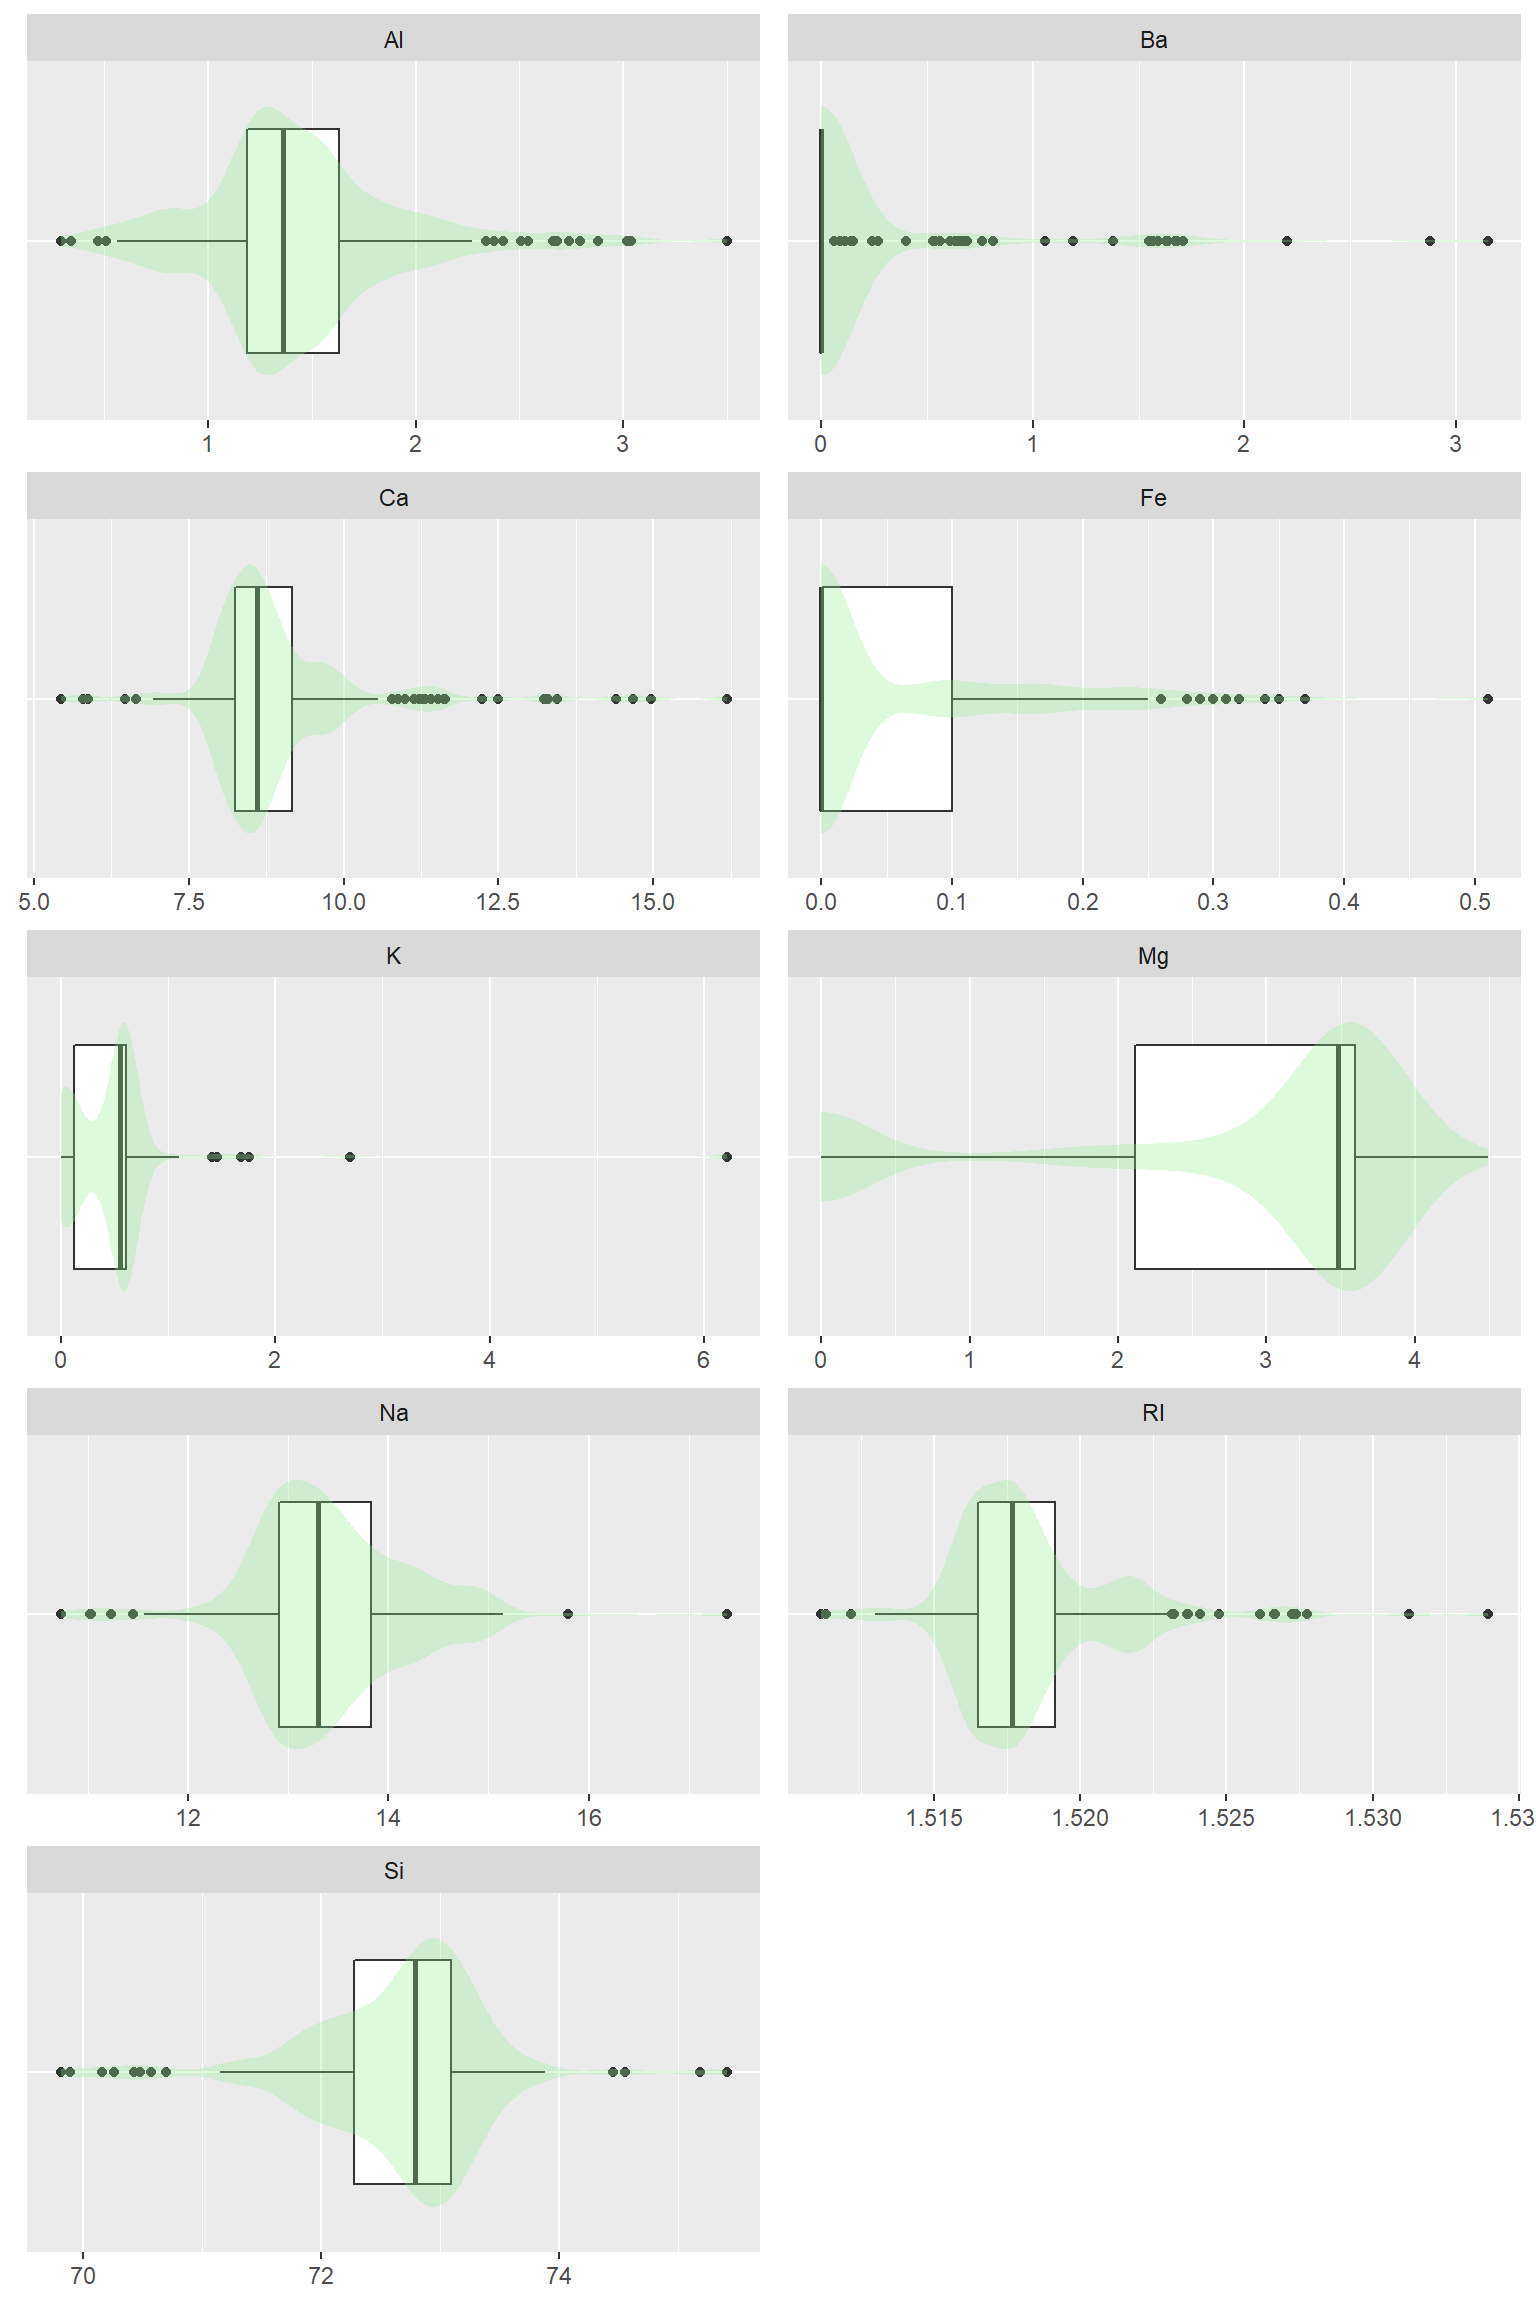
\includegraphics{homework-one_files/figure-latex/facetBox-1} \end{center}

\hypertarget{c.-are-there-any-relevant-transformations-of-one-or-more-predictors-that-might-improve-the-classification-model}{%
\subsection{c. Are there any relevant transformations of one or more predictors that might improve the classification model?}\label{c.-are-there-any-relevant-transformations-of-one-or-more-predictors-that-might-improve-the-classification-model}}

Below we conduct a simple exploration of histograms for skewed distributions using \texttt{BoxCoxTrans(\ )}:

\begin{Shaded}
\begin{Highlighting}[]
\NormalTok{skews <-}\StringTok{ }\KeywordTok{c}\NormalTok{(}\StringTok{"Mg"}\NormalTok{, }\StringTok{"Fe"}\NormalTok{, }\StringTok{"Ba"}\NormalTok{, }\StringTok{"Ca"}\NormalTok{, }\StringTok{"K"}\NormalTok{)}

\CommentTok{# MASS::boxcox(Glass)}
\ControlFlowTok{for}\NormalTok{ (skw }\ControlFlowTok{in}\NormalTok{ skews) \{}
  \KeywordTok{print}\NormalTok{(skw)}
  \KeywordTok{print}\NormalTok{(}\KeywordTok{BoxCoxTrans}\NormalTok{(Glass[, skw]))}
\NormalTok{\}}
\end{Highlighting}
\end{Shaded}

\begin{verbatim}
FALSE [1] "Mg"
FALSE Box-Cox Transformation
FALSE 
FALSE 214 data points used to estimate Lambda
FALSE 
FALSE Input data summary:
FALSE    Min. 1st Qu.  Median    Mean 3rd Qu.    Max. 
FALSE   0.000   2.115   3.480   2.685   3.600   4.490 
FALSE 
FALSE Lambda could not be estimated; no transformation is applied
FALSE 
FALSE [1] "Fe"
FALSE Box-Cox Transformation
FALSE 
FALSE 214 data points used to estimate Lambda
FALSE 
FALSE Input data summary:
FALSE    Min. 1st Qu.  Median    Mean 3rd Qu.    Max. 
FALSE 0.00000 0.00000 0.00000 0.05701 0.10000 0.51000 
FALSE 
FALSE Lambda could not be estimated; no transformation is applied
FALSE 
FALSE [1] "Ba"
FALSE Box-Cox Transformation
FALSE 
FALSE 214 data points used to estimate Lambda
FALSE 
FALSE Input data summary:
FALSE    Min. 1st Qu.  Median    Mean 3rd Qu.    Max. 
FALSE   0.000   0.000   0.000   0.175   0.000   3.150 
FALSE 
FALSE Lambda could not be estimated; no transformation is applied
FALSE 
FALSE [1] "Ca"
FALSE Box-Cox Transformation
FALSE 
FALSE 214 data points used to estimate Lambda
FALSE 
FALSE Input data summary:
FALSE    Min. 1st Qu.  Median    Mean 3rd Qu.    Max. 
FALSE   5.430   8.240   8.600   8.957   9.172  16.190 
FALSE 
FALSE Largest/Smallest: 2.98 
FALSE Sample Skewness: 2.02 
FALSE 
FALSE Estimated Lambda: -1.1 
FALSE 
FALSE [1] "K"
FALSE Box-Cox Transformation
FALSE 
FALSE 214 data points used to estimate Lambda
FALSE 
FALSE Input data summary:
FALSE    Min. 1st Qu.  Median    Mean 3rd Qu.    Max. 
FALSE  0.0000  0.1225  0.5550  0.4971  0.6100  6.2100 
FALSE 
FALSE Lambda could not be estimated; no transformation is applied
\end{verbatim}

A simple log transformation shows improvements in the distribution of the iron variable \texttt{Fe}. However it does introduce outliers on the left; additionally, all the zero values of \texttt{Fe} go to -Inf and are not reflected at all in this distribution.

\begin{Shaded}
\begin{Highlighting}[]
\KeywordTok{par}\NormalTok{(}\DataTypeTok{mfrow =} \KeywordTok{c}\NormalTok{(}\DecValTok{1}\NormalTok{, }\DecValTok{2}\NormalTok{))}
\KeywordTok{hist}\NormalTok{(}\KeywordTok{log}\NormalTok{(Glass}\OperatorTok{$}\NormalTok{Fe), }\DataTypeTok{breaks =} \DecValTok{30}\NormalTok{, }\DataTypeTok{col =} \StringTok{"lightblue"}\NormalTok{, }\DataTypeTok{main =} \StringTok{"Distribution Fe With Log Transformation"}\NormalTok{, }
  \DataTypeTok{xlab =} \StringTok{"Log-transformed Fe"}\NormalTok{)}
\KeywordTok{hist}\NormalTok{(Glass}\OperatorTok{$}\NormalTok{Fe, }\DataTypeTok{breaks =} \DecValTok{30}\NormalTok{, }\DataTypeTok{col =} \StringTok{"gray"}\NormalTok{, }\DataTypeTok{main =} \StringTok{"Fe Without Log Transformation"}\NormalTok{, }
  \DataTypeTok{xlab =} \StringTok{"Fe"}\NormalTok{)}
\end{Highlighting}
\end{Shaded}

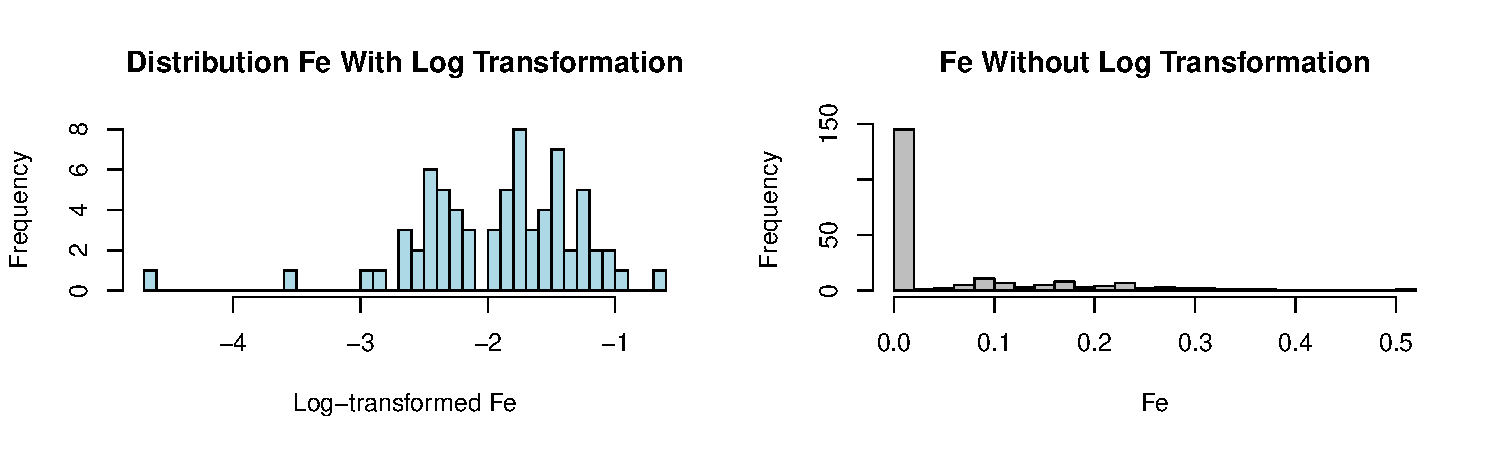
\includegraphics{homework-one_files/figure-latex/3.1c.1-1.pdf}

We then examined the first few rows of the data before and after transformations to see what changes the Box-Cox method suggests.

\begin{Shaded}
\begin{Highlighting}[]
\KeywordTok{head}\NormalTok{(Glass) }\OperatorTok\StringTok{ }\KeywordTok{kable}\NormalTok{(}\DataTypeTok{caption =} \StringTok{"Glass (without transformations)"}\NormalTok{, }
  \DataTypeTok{digits =} \DecValTok{2}\NormalTok{, }\StringTok{"latex"}\NormalTok{) }\OperatorTok\StringTok{ }\KeywordTok{kable_styling}\NormalTok{(}\DataTypeTok{latex_options =} \KeywordTok{c}\NormalTok{(}\StringTok{"hold_position"}\NormalTok{, }
  \StringTok{"striped"}\NormalTok{))}
\end{Highlighting}
\end{Shaded}

\begin{table}[!h]

\caption{\label{tab:before-trans}Glass (without transformations)}
\centering
\fontsize{10}{12}\selectfont
\begin{tabu} to \linewidth {>{\raggedleft}X>{\raggedleft}X>{\raggedleft}X>{\raggedleft}X>{\raggedleft}X>{\raggedleft}X>{\raggedleft}X>{\raggedleft}X>{\raggedleft}X>{\raggedright}X}
\hline
RI & Na & Mg & Al & Si & K & Ca & Ba & Fe & Type\\
\hline
\rowcolor{gray!6}  1.52 & 13.64 & 4.49 & 1.10 & 71.78 & 0.06 & 8.75 & 0 & 0.00 & 1\\
\hline
1.52 & 13.89 & 3.60 & 1.36 & 72.73 & 0.48 & 7.83 & 0 & 0.00 & 1\\
\hline
\rowcolor{gray!6}  1.52 & 13.53 & 3.55 & 1.54 & 72.99 & 0.39 & 7.78 & 0 & 0.00 & 1\\
\hline
1.52 & 13.21 & 3.69 & 1.29 & 72.61 & 0.57 & 8.22 & 0 & 0.00 & 1\\
\hline
\rowcolor{gray!6}  1.52 & 13.27 & 3.62 & 1.24 & 73.08 & 0.55 & 8.07 & 0 & 0.00 & 1\\
\hline
1.52 & 12.79 & 3.61 & 1.62 & 72.97 & 0.64 & 8.07 & 0 & 0.26 & 1\\
\hline
\end{tabu}
\end{table}

\begin{Shaded}
\begin{Highlighting}[]
\NormalTok{trans <-}\StringTok{ }\KeywordTok{preProcess}\NormalTok{(Glass, }\DataTypeTok{method =} \KeywordTok{c}\NormalTok{(}\StringTok{"center"}\NormalTok{, }\StringTok{"scale"}\NormalTok{, }
  \StringTok{"BoxCox"}\NormalTok{))}
\NormalTok{trans_glass <-}\StringTok{ }\KeywordTok{predict}\NormalTok{(trans, Glass)}

\KeywordTok{head}\NormalTok{(trans_glass) }\OperatorTok\StringTok{ }\KeywordTok{kable}\NormalTok{(}\DataTypeTok{caption =} \StringTok{"Glass (with transformations)"}\NormalTok{, }
  \DataTypeTok{digits =} \DecValTok{2}\NormalTok{, }\StringTok{"latex"}\NormalTok{) }\OperatorTok\StringTok{ }\KeywordTok{kable_styling}\NormalTok{(}\DataTypeTok{latex_options =} \KeywordTok{c}\NormalTok{(}\StringTok{"hold_position"}\NormalTok{, }
  \StringTok{"striped"}\NormalTok{))}
\end{Highlighting}
\end{Shaded}

\begin{table}[!h]

\caption{\label{tab:after-trans}Glass (with transformations)}
\centering
\fontsize{10}{12}\selectfont
\begin{tabu} to \linewidth {>{\raggedleft}X>{\raggedleft}X>{\raggedleft}X>{\raggedleft}X>{\raggedleft}X>{\raggedleft}X>{\raggedleft}X>{\raggedleft}X>{\raggedleft}X>{\raggedright}X}
\hline
RI & Na & Mg & Al & Si & K & Ca & Ba & Fe & Type\\
\hline
\rowcolor{gray!6}  0.88 & 0.31 & 1.25 & -0.66 & -1.13 & -0.67 & -0.01 & -0.35 & -0.59 & 1\\
\hline
-0.25 & 0.61 & 0.63 & -0.09 & 0.10 & -0.03 & -0.88 & -0.35 & -0.59 & 1\\
\hline
\rowcolor{gray!6}  -0.72 & 0.18 & 0.60 & 0.27 & 0.44 & -0.16 & -0.93 & -0.35 & -0.59 & 1\\
\hline
-0.23 & -0.22 & 0.70 & -0.23 & -0.06 & 0.11 & -0.49 & -0.35 & -0.59 & 1\\
\hline
\rowcolor{gray!6}  -0.31 & -0.14 & 0.65 & -0.34 & 0.55 & 0.08 & -0.63 & -0.35 & -0.59 & 1\\
\hline
-0.79 & -0.75 & 0.64 & 0.43 & 0.41 & 0.22 & -0.63 & -0.35 & 2.08 & 1\\
\hline
\end{tabu}
\end{table}

Finally, we looked at the histograms of our variables after automated application of the Box-Cox transformations.

\begin{Shaded}
\begin{Highlighting}[]
\NormalTok{trans_glass }\OperatorTok\StringTok{ }\KeywordTok{keep}\NormalTok{(is.numeric) }\OperatorTok\StringTok{ }\KeywordTok{gather}\NormalTok{() }\OperatorTok\StringTok{ }\KeywordTok{ggplot}\NormalTok{(}\KeywordTok{aes}\NormalTok{(value)) }\OperatorTok{+}\StringTok{ }
\StringTok{  }\KeywordTok{facet_wrap}\NormalTok{(}\OperatorTok{~}\NormalTok{key, }\DataTypeTok{scales =} \StringTok{"free"}\NormalTok{) }\OperatorTok{+}\StringTok{ }\KeywordTok{geom_histogram}\NormalTok{(}\DataTypeTok{fill =} \StringTok{"darkorchid"}\NormalTok{, }
  \DataTypeTok{color =} \StringTok{"black"}\NormalTok{) }\OperatorTok{+}\StringTok{ }\KeywordTok{theme_bw}\NormalTok{()}
\end{Highlighting}
\end{Shaded}

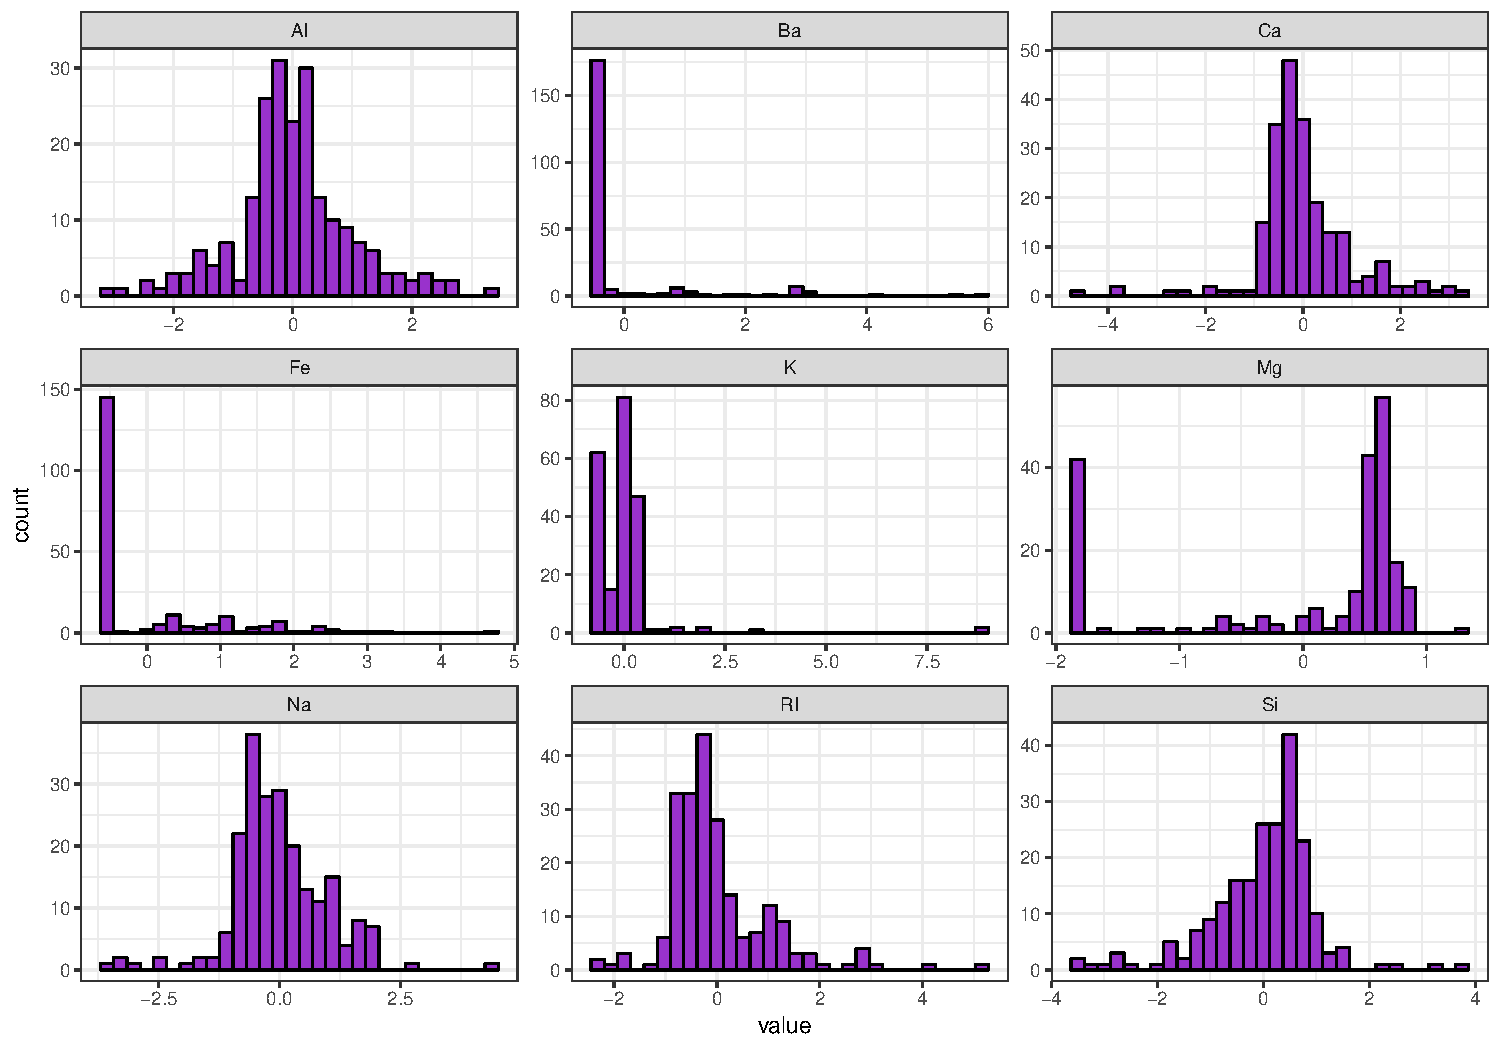
\includegraphics{homework-one_files/figure-latex/3.1c.3-6-1.pdf}

While the transformation produces marginal improvement in most of the variables the only one with noteworthy changes is \texttt{Ca}. Given the number of outliers and skew in this data, it might be useful to attempt a \texttt{spatialSign()} transformation.

\begin{Shaded}
\begin{Highlighting}[]
\NormalTok{trans <-}\StringTok{ }\KeywordTok{preProcess}\NormalTok{(Glass, }\DataTypeTok{method =} \KeywordTok{c}\NormalTok{(}\StringTok{"center"}\NormalTok{, }\StringTok{"scale"}\NormalTok{, }
  \StringTok{"spatialSign"}\NormalTok{))}

\NormalTok{trans_glass <-}\StringTok{ }\KeywordTok{predict}\NormalTok{(trans, Glass)}

\NormalTok{trans_glass }\OperatorTok\StringTok{ }\KeywordTok{keep}\NormalTok{(is.numeric) }\OperatorTok\StringTok{ }\KeywordTok{gather}\NormalTok{() }\OperatorTok\StringTok{ }\KeywordTok{ggplot}\NormalTok{(}\KeywordTok{aes}\NormalTok{(value)) }\OperatorTok{+}\StringTok{ }
\StringTok{  }\KeywordTok{facet_wrap}\NormalTok{(}\OperatorTok{~}\NormalTok{key, }\DataTypeTok{scales =} \StringTok{"free"}\NormalTok{) }\OperatorTok{+}\StringTok{ }\KeywordTok{geom_histogram}\NormalTok{(}\DataTypeTok{fill =} \StringTok{"darkorchid"}\NormalTok{, }
  \DataTypeTok{color =} \StringTok{"black"}\NormalTok{) }\OperatorTok{+}\StringTok{ }\KeywordTok{theme_bw}\NormalTok{()}
\end{Highlighting}
\end{Shaded}

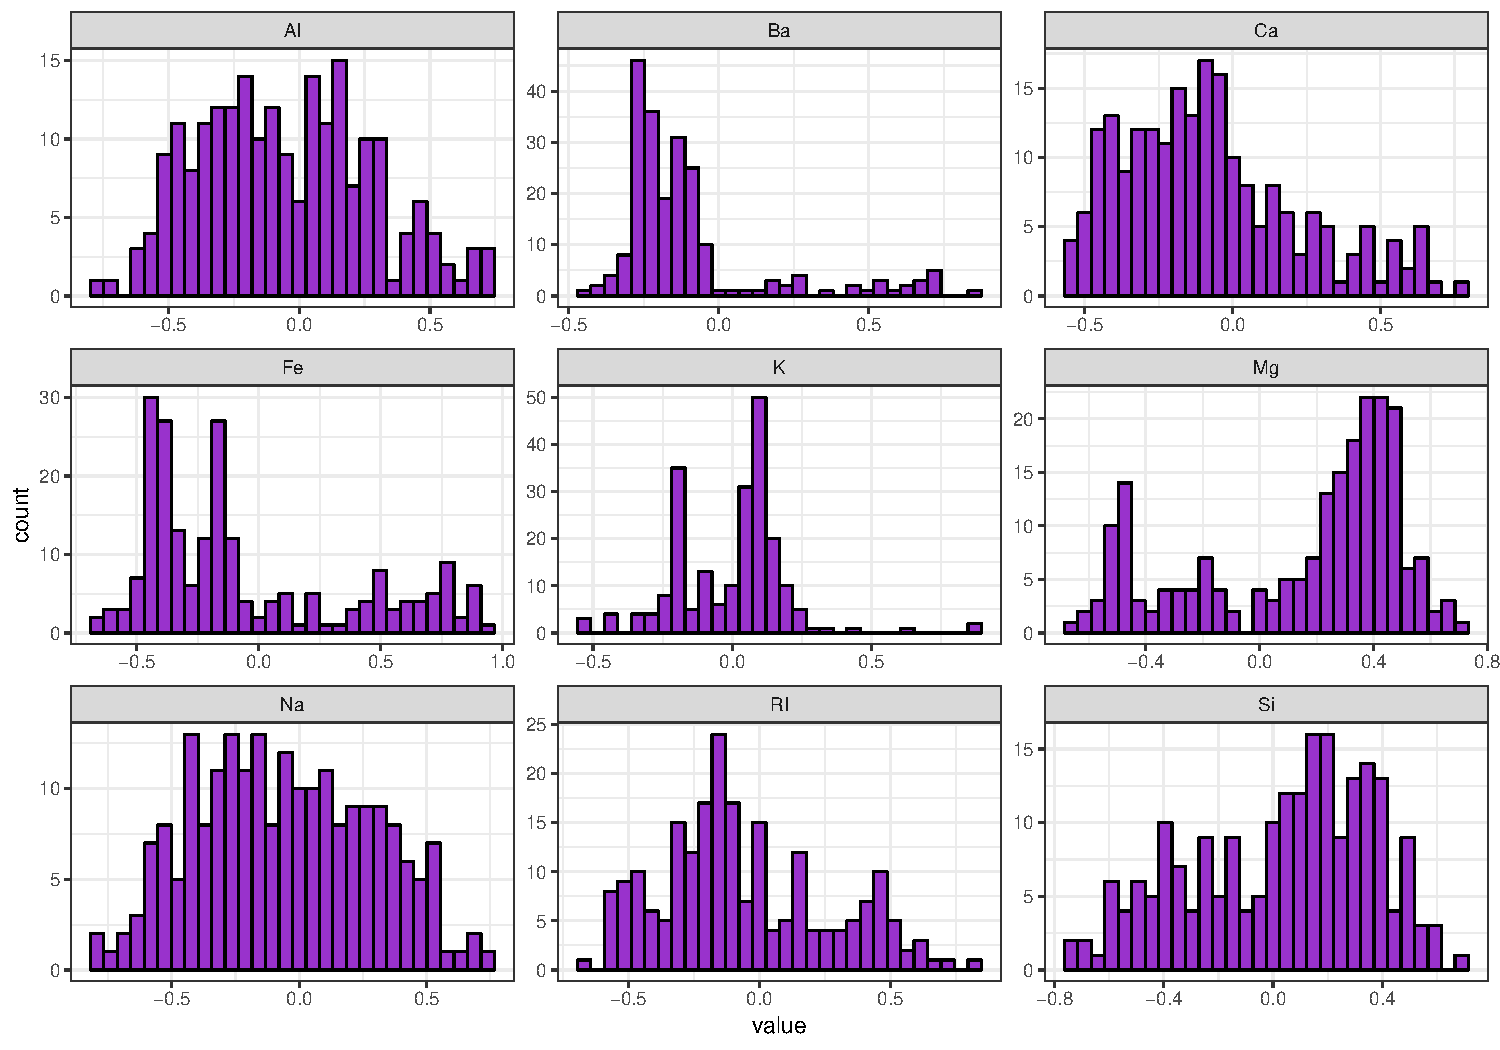
\includegraphics{homework-one_files/figure-latex/ss-1.pdf}
\textbf{Without Spatial Sign:}

\begin{Shaded}
\begin{Highlighting}[]
\KeywordTok{head}\NormalTok{(Glass) }\OperatorTok\StringTok{ }\KeywordTok{kable}\NormalTok{(}\StringTok{"latex"}\NormalTok{, }\DataTypeTok{digits =} \DecValTok{3}\NormalTok{) }\OperatorTok\StringTok{ }\KeywordTok{kable_styling}\NormalTok{(}\DataTypeTok{latex_options =} \StringTok{"hold_position"}\NormalTok{)}
\end{Highlighting}
\end{Shaded}

\begingroup\fontsize{10}{12}\selectfont

\begin{tabu} to \linewidth {>{\raggedleft}X>{\raggedleft}X>{\raggedleft}X>{\raggedleft}X>{\raggedleft}X>{\raggedleft}X>{\raggedleft}X>{\raggedleft}X>{\raggedleft}X>{\raggedright}X}
\hline
RI & Na & Mg & Al & Si & K & Ca & Ba & Fe & Type\\
\hline
1.521 & 13.64 & 4.49 & 1.10 & 71.78 & 0.06 & 8.75 & 0 & 0.00 & 1\\
\hline
1.518 & 13.89 & 3.60 & 1.36 & 72.73 & 0.48 & 7.83 & 0 & 0.00 & 1\\
\hline
1.516 & 13.53 & 3.55 & 1.54 & 72.99 & 0.39 & 7.78 & 0 & 0.00 & 1\\
\hline
1.518 & 13.21 & 3.69 & 1.29 & 72.61 & 0.57 & 8.22 & 0 & 0.00 & 1\\
\hline
1.517 & 13.27 & 3.62 & 1.24 & 73.08 & 0.55 & 8.07 & 0 & 0.00 & 1\\
\hline
1.516 & 12.79 & 3.61 & 1.62 & 72.97 & 0.64 & 8.07 & 0 & 0.26 & 1\\
\hline
\end{tabu}
\endgroup{}

\textbf{With Spatial Sign:}

\begin{Shaded}
\begin{Highlighting}[]
\KeywordTok{head}\NormalTok{(trans_glass) }\OperatorTok\StringTok{ }\KeywordTok{kable}\NormalTok{(}\StringTok{"latex"}\NormalTok{, }\DataTypeTok{digits =} \DecValTok{3}\NormalTok{) }\OperatorTok\StringTok{ }\KeywordTok{kable_styling}\NormalTok{(}\DataTypeTok{latex_options =} \StringTok{"hold_position"}\NormalTok{)}
\end{Highlighting}
\end{Shaded}

\begingroup\fontsize{10}{12}\selectfont

\begin{tabu} to \linewidth {>{\raggedleft}X>{\raggedleft}X>{\raggedleft}X>{\raggedleft}X>{\raggedleft}X>{\raggedleft}X>{\raggedleft}X>{\raggedleft}X>{\raggedleft}X>{\raggedright}X}
\hline
RI & Na & Mg & Al & Si & K & Ca & Ba & Fe & Type\\
\hline
0.386 & 0.126 & 0.555 & -0.306 & -0.499 & -0.297 & -0.064 & -0.156 & -0.259 & 1\\
\hline
-0.178 & 0.423 & 0.455 & -0.122 & 0.073 & -0.019 & -0.568 & -0.252 & -0.419 & 1\\
\hline
-0.474 & 0.099 & 0.395 & 0.125 & 0.288 & -0.108 & -0.545 & -0.232 & -0.385 & 1\\
\hline
-0.193 & -0.202 & 0.580 & -0.258 & -0.044 & 0.093 & -0.431 & -0.293 & -0.487 & 1\\
\hline
-0.227 & -0.123 & 0.473 & -0.299 & 0.404 & 0.059 & -0.454 & -0.257 & -0.426 & 1\\
\hline
-0.304 & -0.290 & 0.246 & 0.134 & 0.158 & 0.084 & -0.239 & -0.135 & 0.799 & 1\\
\hline
\end{tabu}
\endgroup{}

The spatial sign-transformed distributions are the most normal and best for modeling. While custom transformations of each variable might prove even better robust, the simple spatial sign grooming and pre-processing method seems practical and useful for this data set.

\hypertarget{kuhn-johnson-3.2}{%
\section{Kuhn \& Johnson 3.2}\label{kuhn-johnson-3.2}}

\begin{quote}
The soybean data can also be found at the UC Irvine Machine Learning Repository. Data were collected to predict disease in 683 soybeans. The 35 predictors are mostly categorical and include information on the environmental conditions (e.g.~temperature, precipitation) and plant conditions (e.g.~left spots, mold growth). The outcome labels consist of 19 distinct classes.
\end{quote}

\begin{Shaded}
\begin{Highlighting}[]
\KeywordTok{data}\NormalTok{(Soybean)}
\CommentTok{# str(Soybean)}
\end{Highlighting}
\end{Shaded}

\hypertarget{a.-investigate-the-frequency-distributions-for-the-categorical-predictors.-are-any-of-the-distributions-degenerate-in-the-ways-discussed-earlier-in-this-chapter}{%
\subsection{a. Investigate the frequency distributions for the categorical predictors. Are any of the distributions degenerate in the ways discussed earlier in this chapter?}\label{a.-investigate-the-frequency-distributions-for-the-categorical-predictors.-are-any-of-the-distributions-degenerate-in-the-ways-discussed-earlier-in-this-chapter}}

\begin{Shaded}
\begin{Highlighting}[]
\CommentTok{# Tidy dataset, removing non-numeric variables}
\NormalTok{Soybean }\OperatorTok\StringTok{ }\KeywordTok{select}\NormalTok{(}\OperatorTok{-}\NormalTok{Class) }\OperatorTok\StringTok{ }\KeywordTok{gather}\NormalTok{() }\OperatorTok\StringTok{ }
\CommentTok{# Depict distribution of each class within categories}
\KeywordTok{ggplot}\NormalTok{(}\KeywordTok{aes}\NormalTok{(value, }\DataTypeTok{fill =}\NormalTok{ value)) }\OperatorTok{+}\StringTok{ }\KeywordTok{geom_bar}\NormalTok{() }\OperatorTok{+}\StringTok{ }
\CommentTok{# Code all 0 factor values as red for easier visual}
\CommentTok{# detection of degenerate distribution}
\KeywordTok{scale_fill_manual}\NormalTok{(}\DataTypeTok{values =} \KeywordTok{c}\NormalTok{(}\StringTok{"red"}\NormalTok{, }\KeywordTok{rep}\NormalTok{(}\StringTok{"grey40"}\NormalTok{, }\DecValTok{7}\NormalTok{))) }\OperatorTok{+}\StringTok{ }
\StringTok{  }
\CommentTok{# Facet plots by predictor and attenuate chart look}
\KeywordTok{facet_wrap}\NormalTok{(}\OperatorTok{~}\NormalTok{key) }\OperatorTok{+}\StringTok{ }\KeywordTok{theme_minimal}\NormalTok{() }\OperatorTok{+}\StringTok{ }\KeywordTok{labs}\NormalTok{(}\DataTypeTok{title =} \StringTok{"Soybean: Distributions by Predictor"}\NormalTok{)}
\end{Highlighting}
\end{Shaded}

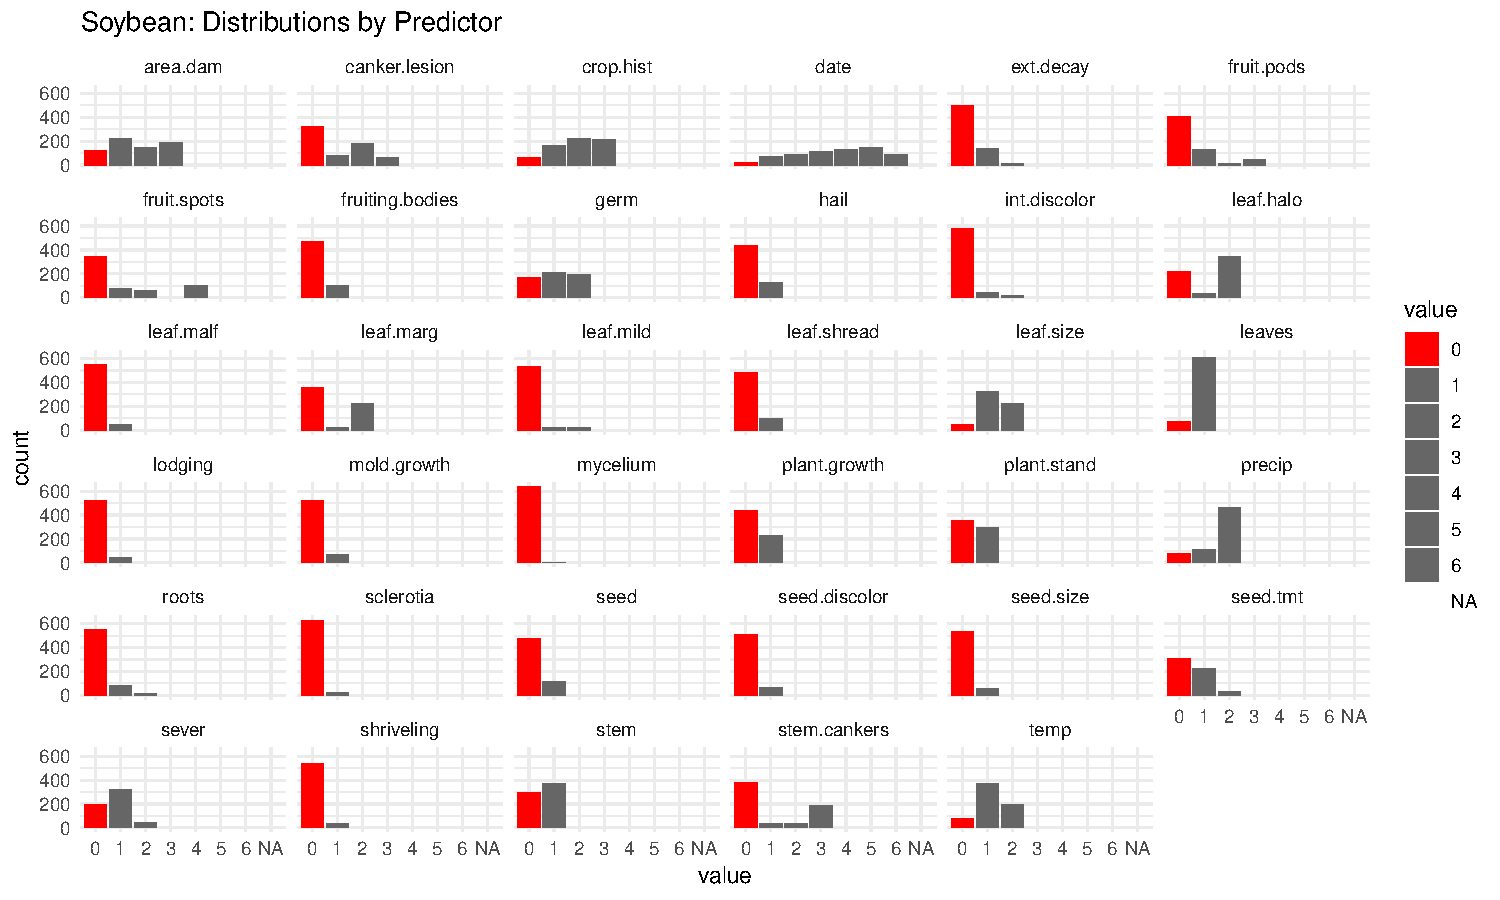
\includegraphics{homework-one_files/figure-latex/kj3.2a-1.pdf}

Distributions are regarded as degenerate when they have a unique values with extremely low frequencies, i.e. `predictors with a single value for the vast majority of samples'. \texttt{mycelium} and \texttt{sclerotica} both fall into this category, and arguably \texttt{leaf.mild}, \texttt{lodging}, \texttt{seed.discolor}, \texttt{seed.size}, and \texttt{shriveling} could also be considered.

\hypertarget{b.-roughly-18-of-the-data-are-missing.-are-there-particular-predictors-that-are-more-likely-to-be-missing-is-the-pattern-of-missing-data-related-to-the-classes}{%
\subsection{b. Roughly 18\% of the data are missing. Are there particular predictors that are more likely to be missing? Is the pattern of missing data related to the classes?**}\label{b.-roughly-18-of-the-data-are-missing.-are-there-particular-predictors-that-are-more-likely-to-be-missing-is-the-pattern-of-missing-data-related-to-the-classes}}

\begin{Shaded}
\begin{Highlighting}[]
\CommentTok{# Tidy dataset, removing non-numeric variables}
\NormalTok{Soybean }\OperatorTok\StringTok{ }\KeywordTok{select}\NormalTok{(}\OperatorTok{-}\NormalTok{Class, }\OperatorTok{-}\NormalTok{date) }\OperatorTok\StringTok{ }\KeywordTok{summarise_all}\NormalTok{(}\KeywordTok{funs}\NormalTok{(}\DataTypeTok{perc_missing =} \KeywordTok{sum}\NormalTok{(}\KeywordTok{is.na}\NormalTok{((.))}\OperatorTok{/}\KeywordTok{nrow}\NormalTok{(Soybean)))) }\OperatorTok\StringTok{ }
\StringTok{  }\KeywordTok{rename_all}\NormalTok{(}\KeywordTok{funs}\NormalTok{(}\KeywordTok{str_replace}\NormalTok{(., }\StringTok{"_perc_missing"}\NormalTok{, }\StringTok{""}\NormalTok{))) }\OperatorTok\StringTok{ }
\StringTok{  }\KeywordTok{gather}\NormalTok{() }\OperatorTok\StringTok{ }\KeywordTok{ggplot}\NormalTok{(}\KeywordTok{aes}\NormalTok{(}\DataTypeTok{x =} \KeywordTok{reorder}\NormalTok{(key, value), }\DataTypeTok{y =}\NormalTok{ value)) }\OperatorTok{+}\StringTok{ }
\StringTok{  }\KeywordTok{geom_bar}\NormalTok{(}\DataTypeTok{stat =} \StringTok{"identity"}\NormalTok{, }\DataTypeTok{fill =} \StringTok{"grey40"}\NormalTok{) }\OperatorTok{+}\StringTok{ }\CommentTok{# Annotate bar chart with percentage missing}
\KeywordTok{geom_text}\NormalTok{(}\KeywordTok{aes}\NormalTok{(}\DataTypeTok{label =}\NormalTok{ scales}\OperatorTok{::}\KeywordTok{percent}\NormalTok{(value), }\DataTypeTok{y =} \FloatTok{-0.01}\NormalTok{), }
  \DataTypeTok{size =} \DecValTok{3}\NormalTok{, }\DataTypeTok{position =} \KeywordTok{position_dodge}\NormalTok{(}\DataTypeTok{width =} \FloatTok{0.9}\NormalTok{)) }\OperatorTok{+}\StringTok{ }\KeywordTok{coord_flip}\NormalTok{() }\OperatorTok{+}\StringTok{ }
\StringTok{  }\KeywordTok{labs}\NormalTok{(}\DataTypeTok{title =} \StringTok{"Soybean: Missing Data by Predictor"}\NormalTok{, }\DataTypeTok{x =} \StringTok{""}\NormalTok{, }
    \DataTypeTok{y =} \StringTok{""}\NormalTok{) }\OperatorTok{+}\StringTok{ }\KeywordTok{theme_bw}\NormalTok{() }\OperatorTok{+}\StringTok{ }\KeywordTok{theme}\NormalTok{(}\DataTypeTok{axis.text.x =} \KeywordTok{element_blank}\NormalTok{())}
\end{Highlighting}
\end{Shaded}

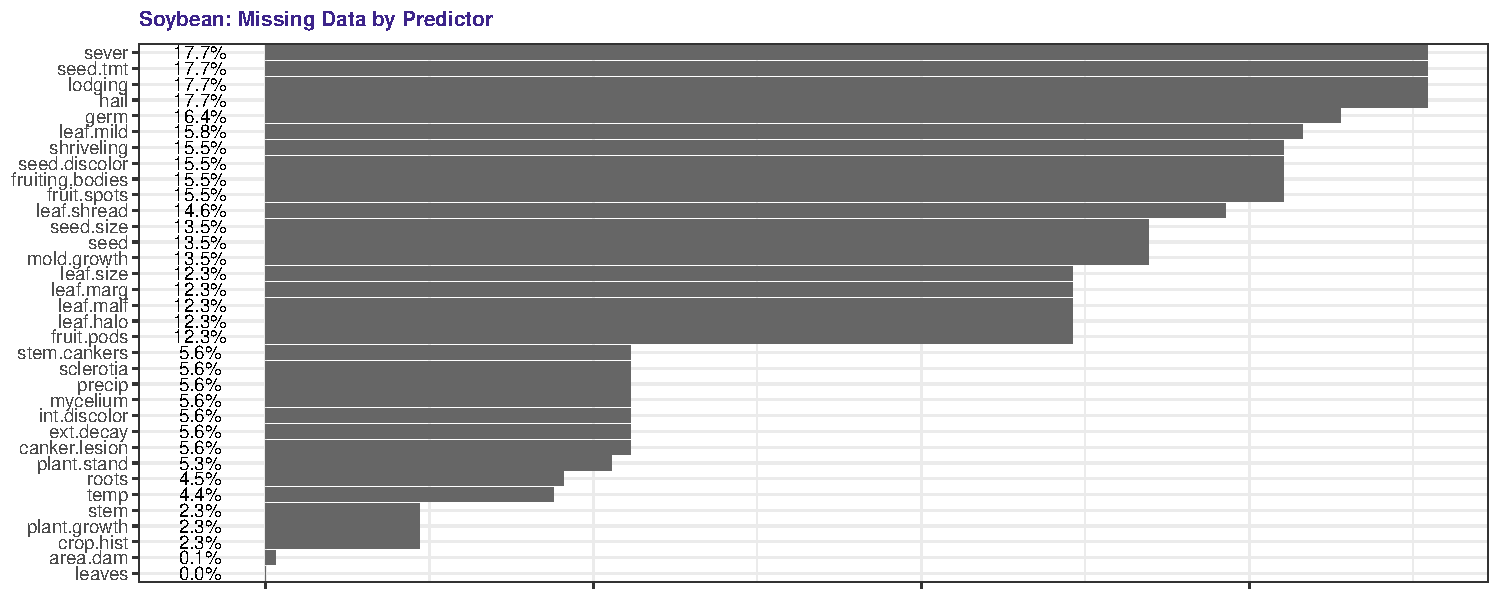
\includegraphics{homework-one_files/figure-latex/kj3.2b1-1.pdf}

Of the 18\% of incomplete cases, the predictors \texttt{sever}, \texttt{seed.tmt}, and \texttt{lodging}, and \texttt{hail} are missing in almost all of them.

Apart from \texttt{Class} and \texttt{date}, \texttt{leaves} is the only other predictor that's present for all cases.

\begin{Shaded}
\begin{Highlighting}[]
\KeywordTok{kable}\NormalTok{(}\KeywordTok{table}\NormalTok{(Soybean}\OperatorTok{$}\NormalTok{Class, }\KeywordTok{complete.cases}\NormalTok{(Soybean)), }\DataTypeTok{caption =} \StringTok{"NA Values"}\NormalTok{, }
  \StringTok{"latex"}\NormalTok{) }\OperatorTok\StringTok{ }\KeywordTok{kable_styling}\NormalTok{(}\DataTypeTok{latex_options =} \KeywordTok{c}\NormalTok{(}\StringTok{"hold_position"}\NormalTok{, }
  \StringTok{"striped"}\NormalTok{))}
\end{Highlighting}
\end{Shaded}

\begin{table}[!h]

\caption{\label{tab:unnamed-chunk-3}NA Values}
\centering
\fontsize{10}{12}\selectfont
\begin{tabu} to \linewidth {>{\raggedright}X>{\raggedleft}X>{\raggedleft}X}
\hline
  & FALSE & TRUE\\
\hline
\rowcolor{gray!6}  2-4-d-injury & 16 & 0\\
\hline
alternarialeaf-spot & 0 & 91\\
\hline
\rowcolor{gray!6}  anthracnose & 0 & 44\\
\hline
bacterial-blight & 0 & 20\\
\hline
\rowcolor{gray!6}  bacterial-pustule & 0 & 20\\
\hline
brown-spot & 0 & 92\\
\hline
\rowcolor{gray!6}  brown-stem-rot & 0 & 44\\
\hline
charcoal-rot & 0 & 20\\
\hline
\rowcolor{gray!6}  cyst-nematode & 14 & 0\\
\hline
diaporthe-pod-\&-stem-blight & 15 & 0\\
\hline
\rowcolor{gray!6}  diaporthe-stem-canker & 0 & 20\\
\hline
downy-mildew & 0 & 20\\
\hline
\rowcolor{gray!6}  frog-eye-leaf-spot & 0 & 91\\
\hline
herbicide-injury & 8 & 0\\
\hline
\rowcolor{gray!6}  phyllosticta-leaf-spot & 0 & 20\\
\hline
phytophthora-rot & 68 & 20\\
\hline
\rowcolor{gray!6}  powdery-mildew & 0 & 20\\
\hline
purple-seed-stain & 0 & 20\\
\hline
\rowcolor{gray!6}  rhizoctonia-root-rot & 0 & 20\\
\hline
\end{tabu}
\end{table}

We should check to see if this is the result of chance, or if there are systematic issues (i.e.~the data generating process, measurement challenges, recording errors, data loss, etc.) that could explain this.

\begin{Shaded}
\begin{Highlighting}[]
\CommentTok{# Calculate total cases in Soybean set}
\NormalTok{total_cases <-}\StringTok{ }\KeywordTok{nrow}\NormalTok{(Soybean)}

\CommentTok{# Tidy dataset, calculating complete cases by predictor}
\CommentTok{# and predictor cases overall}
\NormalTok{Soybean }\OperatorTok\StringTok{ }\KeywordTok{mutate}\NormalTok{(}\DataTypeTok{complete_cases =} \KeywordTok{complete.cases}\NormalTok{(Soybean)) }\OperatorTok\StringTok{ }
\StringTok{  }\KeywordTok{group_by}\NormalTok{(Class) }\OperatorTok\StringTok{ }\KeywordTok{summarize}\NormalTok{(}\DataTypeTok{cases =} \KeywordTok{n}\NormalTok{(), }\DataTypeTok{complete_cases =} \KeywordTok{sum}\NormalTok{(complete_cases), }
  \DataTypeTok{completeness =}\NormalTok{ complete_cases}\OperatorTok{/}\NormalTok{cases, }\DataTypeTok{proportion_allcases =}\NormalTok{ cases}\OperatorTok{/}\NormalTok{total_cases) }\OperatorTok\StringTok{ }
\StringTok{  }
\CommentTok{# Display only predictors with missing data}
\KeywordTok{filter}\NormalTok{(completeness }\OperatorTok{!=}\StringTok{ }\DecValTok{1}\NormalTok{) }\OperatorTok\StringTok{ }\KeywordTok{arrange}\NormalTok{(}\KeywordTok{desc}\NormalTok{(proportion_allcases)) }\OperatorTok\StringTok{ }
\StringTok{  }
\CommentTok{# Attenuate table look}
\KeywordTok{mutate}\NormalTok{(}\DataTypeTok{completeness =}\NormalTok{ scales}\OperatorTok{::}\KeywordTok{percent}\NormalTok{(completeness), }\DataTypeTok{proportion_allcases =}\NormalTok{ scales}\OperatorTok{::}\KeywordTok{percent}\NormalTok{(proportion_allcases)) }\OperatorTok\StringTok{ }
\StringTok{  }\KeywordTok{select}\NormalTok{(Class, cases, complete_cases, completeness, proportion_allcases) }\OperatorTok\StringTok{ }
\StringTok{  }\KeywordTok{rename}\NormalTok{(}\DataTypeTok{class =}\NormalTok{ Class) }\OperatorTok\StringTok{ }\KeywordTok{kable}\NormalTok{(}\DataTypeTok{caption =} \StringTok{"Complete Cases"}\NormalTok{, }
  \DataTypeTok{label =} \OtherTok{NULL}\NormalTok{, }\StringTok{"latex"}\NormalTok{) }\OperatorTok\StringTok{ }\KeywordTok{kable_styling}\NormalTok{(}\DataTypeTok{latex_options =} \KeywordTok{c}\NormalTok{(}\StringTok{"hold_position"}\NormalTok{, }
  \StringTok{"striped"}\NormalTok{))}
\end{Highlighting}
\end{Shaded}

\begin{table}[!h]

\caption{\label{tab:completeness}Complete Cases}
\centering
\fontsize{10}{12}\selectfont
\begin{tabu} to \linewidth {>{\raggedright}X>{\raggedleft}X>{\raggedleft}X>{\raggedright}X>{\raggedright}X}
\hline
class & cases & complete\_cases & completeness & proportion\_allcases\\
\hline
\rowcolor{gray!6}  phytophthora-rot & 88 & 20 & 22.7\% & 12.9\%\\
\hline
2-4-d-injury & 16 & 0 & 0.0\% & 2.3\%\\
\hline
\rowcolor{gray!6}  diaporthe-pod-\&-stem-blight & 15 & 0 & 0.0\% & 2.2\%\\
\hline
cyst-nematode & 14 & 0 & 0.0\% & 2.0\%\\
\hline
\rowcolor{gray!6}  herbicide-injury & 8 & 0 & 0.0\% & 1.2\%\\
\hline
\end{tabu}
\end{table}

When completeness is examined from the viewpoint of \texttt{Class}, it becomes apparent that five classes are responsible for all missing data: \texttt{phytophthora-rot}, \texttt{2-4-d-injury}, \texttt{diaporthe-pod-\&-stem-blight}, \texttt{cyst-nematode}, and \texttt{herbicide-injury}. Diagnosis of the cause of missing data should focus on these classes.

\hypertarget{c.-develop-a-strategy-for-handling-missing-data-either-by-eliminating-predictors-or-imputation.}{%
\subsection{c. Develop a strategy for handling missing data, either by eliminating predictors or imputation.**}\label{c.-develop-a-strategy-for-handling-missing-data-either-by-eliminating-predictors-or-imputation.}}

There is no simple method for handling missing data AND preserving the global utility of it. Because the classes with missing data have many incomplete cases in the observations, imputation that could be useful for the less empty classes would introduce a lot of error for the more empty ones.

If performing imputation, it would be important to create a new, separate flag variable so that models with high sensitivity can use native values differently than imputed ones (attributing bias to the `flag') - an approach we have used in logistic regression with some success. It may also be useful to reduce dimensionality by extracting the most variance through PCA or LDA.

Additionally, purging the most empty four or five classes and impute the remainder could be a beneficial approach. Alternatively, we might remove the four emptiest classes, establish which variables are most important using PCA, and then see how those variables are represented by the four fragile classes with high NA counts; if those classes are less impacted, it might be possible to impute across the remaining variables for all classes using flags for the imputed values and preserving a good amount of predictive power.

\hypertarget{assignment-four}{%
\chapter{Assignment Four}\label{assignment-four}}

\begin{itemize}
\tightlist
\item
  Hyndman 7.1\\
\item
  Hyndman 7.3
\end{itemize}

\hypertarget{hyndman-7.1}{%
\section{Hyndman 7.1}\label{hyndman-7.1}}

\begin{quote}
Consider the \texttt{pigs} series -- the number of pigs slaughtered in Victoria each month.
\end{quote}

\hypertarget{a.-use-the-ses-function-in-r-to-find-the-optimal-values-of-alpha-and-ell_0-and-generate-forecasts-for-the-next-four-months.}{%
\subsection{\texorpdfstring{a. Use the \texttt{ses()} function in R to find the optimal values of \(\alpha\) and \(\ell_0\), and generate forecasts for the next four months.}{a. Use the ses() function in R to find the optimal values of \textbackslash{}alpha and \textbackslash{}ell\_0, and generate forecasts for the next four months.}}\label{a.-use-the-ses-function-in-r-to-find-the-optimal-values-of-alpha-and-ell_0-and-generate-forecasts-for-the-next-four-months.}}

\hypertarget{forecast-summary}{%
\subsubsection{Forecast Summary}\label{forecast-summary}}

The forecast summary below shows us the optimal values of \(\alpha\) and \(\ell_0\), as estimated by the \texttt{ses} function in R.

\begin{Shaded}
\begin{Highlighting}[]
\NormalTok{pigsdata <-}\StringTok{ }\KeywordTok{window}\NormalTok{(pigs, }\DataTypeTok{start=}\DecValTok{1980}\NormalTok{)}
\NormalTok{fc <-}\StringTok{ }\KeywordTok{ses}\NormalTok{(pigsdata, }\DataTypeTok{h=}\DecValTok{4}\NormalTok{)}
\KeywordTok{summary}\NormalTok{(fc) }
\end{Highlighting}
\end{Shaded}

\begin{verbatim}
FALSE 
FALSE Forecast method: Simple exponential smoothing
FALSE 
FALSE Model Information:
FALSE Simple exponential smoothing 
FALSE 
FALSE Call:
FALSE  ses(y = pigsdata, h = 4) 
FALSE 
FALSE   Smoothing parameters:
FALSE     alpha = 0.2971 
FALSE 
FALSE   Initial states:
FALSE     l = 77260.0561 
FALSE 
FALSE   sigma:  10308.58
FALSE 
FALSE      AIC     AICc      BIC 
FALSE 4462.955 4463.086 4472.665 
FALSE 
FALSE Error measures:
FALSE                    ME    RMSE      MAE       MPE
FALSE Training set 385.8721 10253.6 7961.383 -0.922652
FALSE                  MAPE      MASE       ACF1
FALSE Training set 9.274016 0.7966249 0.01282239
FALSE 
FALSE Forecasts:
FALSE          Point Forecast    Lo 80    Hi 80    Lo 95
FALSE Sep 1995       98816.41 85605.43 112027.4 78611.97
FALSE Oct 1995       98816.41 85034.52 112598.3 77738.83
FALSE Nov 1995       98816.41 84486.34 113146.5 76900.46
FALSE Dec 1995       98816.41 83958.37 113674.4 76092.99
FALSE             Hi 95
FALSE Sep 1995 119020.8
FALSE Oct 1995 119894.0
FALSE Nov 1995 120732.4
FALSE Dec 1995 121539.8
\end{verbatim}

\hypertarget{visualization}{%
\subsubsection{Visualization}\label{visualization}}

\begin{Shaded}
\begin{Highlighting}[]
\KeywordTok{autoplot}\NormalTok{(fc) }\OperatorTok{+}\StringTok{ }\KeywordTok{autolayer}\NormalTok{(}\KeywordTok{fitted}\NormalTok{(fc), }\DataTypeTok{series =} \StringTok{"Fitted"}\NormalTok{) }\OperatorTok{+}\StringTok{ }
\StringTok{  }\KeywordTok{ylab}\NormalTok{(}\StringTok{"Pigs"}\NormalTok{) }\OperatorTok{+}\StringTok{ }\KeywordTok{xlab}\NormalTok{(}\StringTok{"Year"}\NormalTok{) }\OperatorTok{+}\StringTok{ }\KeywordTok{theme_bw}\NormalTok{() }\OperatorTok{+}\StringTok{ }\KeywordTok{theme}\NormalTok{()}
\end{Highlighting}
\end{Shaded}

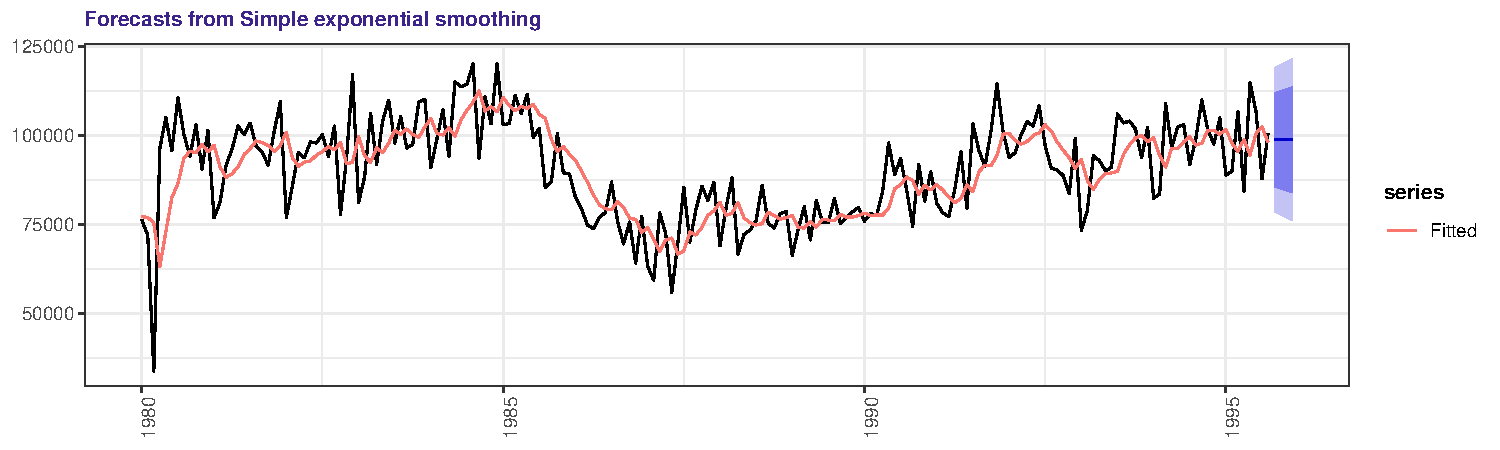
\includegraphics{homework-one_files/figure-latex/ha-7.1a2-1.pdf}

\hypertarget{b.-compute-a-95-prediction-interval-for-the-first-forecast-using-hatypm1.96s-where-s-is-the-standard-deviation-of-the-residuals.-compare-your-interval-with-the-interval-produced-by-r.}{%
\subsection{\texorpdfstring{b. Compute a 95\% prediction interval for the first forecast using \(\hat{y}\pm1.96s\) where \(s\) is the standard deviation of the residuals. Compare your interval with the interval produced by R.}{b. Compute a 95\% prediction interval for the first forecast using \textbackslash{}hat\{y\}\textbackslash{}pm1.96s where s is the standard deviation of the residuals. Compare your interval with the interval produced by R.}}\label{b.-compute-a-95-prediction-interval-for-the-first-forecast-using-hatypm1.96s-where-s-is-the-standard-deviation-of-the-residuals.-compare-your-interval-with-the-interval-produced-by-r.}}

Formula calculations of the confidence interval were obtained using \(\bar{x} \pm 1.96s\) and compared to the calculations from the \texttt{ses} function in R.

\begin{Shaded}
\begin{Highlighting}[]
\CommentTok{# Formula Calculatioin}
\NormalTok{lower <-}\StringTok{ }\NormalTok{fc}\OperatorTok{$}\NormalTok{mean[}\DecValTok{1}\NormalTok{] }\OperatorTok{-}\StringTok{ }\FloatTok{1.96} \OperatorTok{*}\StringTok{ }\KeywordTok{sd}\NormalTok{(fc}\OperatorTok{$}\NormalTok{residuals)}
\NormalTok{upper <-}\StringTok{ }\NormalTok{fc}\OperatorTok{$}\NormalTok{mean[}\DecValTok{1}\NormalTok{] }\OperatorTok{+}\StringTok{ }\FloatTok{1.96} \OperatorTok{*}\StringTok{ }\KeywordTok{sd}\NormalTok{(fc}\OperatorTok{$}\NormalTok{residuals)}

\CommentTok{# R Calculation}
\NormalTok{lowerR <-}\StringTok{ }\KeywordTok{as.numeric}\NormalTok{(fc}\OperatorTok{$}\NormalTok{lower[}\DecValTok{1}\NormalTok{, }\StringTok{"95%"}\NormalTok{])}
\NormalTok{upperR <-}\StringTok{ }\KeywordTok{as.numeric}\NormalTok{(fc}\OperatorTok{$}\NormalTok{upper[}\DecValTok{1}\NormalTok{, }\StringTok{"95%"}\NormalTok{])}

\CommentTok{# Table Output}
\NormalTok{lower <-}\StringTok{ }\KeywordTok{cbind}\NormalTok{(}\StringTok{`}\DataTypeTok{95_perct}\StringTok{`}\NormalTok{ =}\StringTok{ "Lower"}\NormalTok{, }\DataTypeTok{Computed =}\NormalTok{ lower, }\DataTypeTok{R =}\NormalTok{ lowerR)}
\NormalTok{upper <-}\StringTok{ }\KeywordTok{cbind}\NormalTok{(}\StringTok{`}\DataTypeTok{95_perct}\StringTok{`}\NormalTok{ =}\StringTok{ "Upper"}\NormalTok{, }\DataTypeTok{Computed =}\NormalTok{ upper, }\DataTypeTok{R =}\NormalTok{ upperR)}
\KeywordTok{as.data.frame}\NormalTok{(}\KeywordTok{rbind}\NormalTok{(lower, upper)) }\OperatorTok\StringTok{ }\KeywordTok{kable}\NormalTok{(}\StringTok{"latex"}\NormalTok{) }\OperatorTok\StringTok{ }
\StringTok{  }\KeywordTok{kable_styling}\NormalTok{(}\DataTypeTok{latex_options =} \StringTok{"hold_position"}\NormalTok{)}
\end{Highlighting}
\end{Shaded}

\begingroup\fontsize{10}{12}\selectfont

\begin{tabu} to \linewidth {>{\raggedright}X>{\raggedright}X>{\raggedright}X}
\hline
95\_perct & Computed & R\\
\hline
Lower & 78679.9672534162 & 78611.9684577467\\
\hline
Upper & 118952.844969765 & 119020.843765435\\
\hline
\end{tabu}
\endgroup{}

\hypertarget{hyndman-7.3}{%
\section{Hyndman 7.3}\label{hyndman-7.3}}

\begin{quote}
Modify your function from the previous exercise to return the sum of squared errors rather than the forecast of the next observation. Then use the \texttt{optim()} function to find the optimal values of \(\alpha\) and \(\ell_0\). Do you get the same values as the \texttt{ses()} function?
\end{quote}

\hypertarget{function}{%
\subsubsection{Function}\label{function}}

The prior question asks us to write a function to implement simple exponential smoothing. As this was a challenge, we made reference to \href{https://stats.stackexchange.com/questions/379727/how-to-use-optim-function-in-r-on-my-custom-residual-sum-of-squares-function}{stackexchange} while crafting what follows.

\begin{Shaded}
\begin{Highlighting}[]
\CommentTok{# Custom SES Function}
\NormalTok{custom_ses =}\StringTok{ }\ControlFlowTok{function}\NormalTok{(ts, alpha, l0) \{}
\NormalTok{  N =}\StringTok{ }\KeywordTok{length}\NormalTok{(ts)}
\NormalTok{  y_hat =}\StringTok{ }\KeywordTok{c}\NormalTok{(l0, }\DecValTok{0} \OperatorTok{*}\StringTok{ }\NormalTok{(}\DecValTok{2}\OperatorTok{:}\NormalTok{N))}
  \ControlFlowTok{for}\NormalTok{ (j }\ControlFlowTok{in} \DecValTok{1}\OperatorTok{:}\NormalTok{(N }\OperatorTok{-}\StringTok{ }\DecValTok{1}\NormalTok{)) \{}
\NormalTok{    new =}\StringTok{ }\NormalTok{alpha }\OperatorTok{*}\StringTok{ }\NormalTok{ts[j] }\OperatorTok{+}\StringTok{ }\NormalTok{(}\DecValTok{1} \OperatorTok{-}\StringTok{ }\NormalTok{alpha) }\OperatorTok{*}\StringTok{ }\NormalTok{y_hat[j]}
\NormalTok{    y_hat[j }\OperatorTok{+}\StringTok{ }\DecValTok{1}\NormalTok{] =}\StringTok{ }\NormalTok{new}
\NormalTok{  \}}
  \KeywordTok{return}\NormalTok{(y_hat)}
\NormalTok{\}}

\CommentTok{# SSE function}
\NormalTok{custom_sse =}\StringTok{ }\ControlFlowTok{function}\NormalTok{(fn, ts) \{}
\NormalTok{  alpha <-}\StringTok{ }\NormalTok{fn[}\DecValTok{1}\NormalTok{]}
\NormalTok{  l0 <-}\StringTok{ }\NormalTok{fn[}\DecValTok{2}\NormalTok{]}
\NormalTok{  N =}\StringTok{ }\KeywordTok{length}\NormalTok{(ts)}
\NormalTok{  fit =}\StringTok{ }\KeywordTok{custom_ses}\NormalTok{(ts, alpha, l0)}
\NormalTok{  res =}\StringTok{ }\NormalTok{ts }\OperatorTok{-}\StringTok{ }\NormalTok{fit}
\NormalTok{  out =}\StringTok{ }\KeywordTok{sum}\NormalTok{(res}\OperatorTok{^}\DecValTok{2}\NormalTok{)}\OperatorTok{/}\NormalTok{(N }\OperatorTok{-}\StringTok{ }\DecValTok{1}\NormalTok{)}
  \KeywordTok{return}\NormalTok{(out)}
\NormalTok{\}}
\end{Highlighting}
\end{Shaded}

\hypertarget{optimization}{%
\subsubsection{Optimization}\label{optimization}}

The \texttt{optim} function optimizes the parameters \(\alpha\) and \(\ell_0\) by using the initial values in the \texttt{par} argument to maximize output from the vector defined in our custom functions.

\begin{Shaded}
\begin{Highlighting}[]
\CommentTok{# `optim` Function}
\NormalTok{optimize <-}\StringTok{ }\KeywordTok{optim}\NormalTok{(}\DataTypeTok{par =} \KeywordTok{c}\NormalTok{(}\FloatTok{0.1}\NormalTok{, }\DecValTok{10000}\NormalTok{), }\DataTypeTok{fn =}\NormalTok{ custom_sse, }\DataTypeTok{ts =}\NormalTok{ pigsdata)}

\CommentTok{# Optimized Parameters}
\NormalTok{alpha =}\StringTok{ }\NormalTok{optimize}\OperatorTok{$}\NormalTok{par[}\DecValTok{1}\NormalTok{]}
\NormalTok{l0 =}\StringTok{ }\NormalTok{optimize}\OperatorTok{$}\NormalTok{par[}\DecValTok{2}\NormalTok{]}

\CommentTok{# SES Model Parameters}
\NormalTok{ses_alpha <-}\StringTok{ }\NormalTok{fc}\OperatorTok{$}\NormalTok{model}\OperatorTok{$}\NormalTok{fit}\OperatorTok{$}\NormalTok{par[}\DecValTok{1}\NormalTok{]}
\NormalTok{ses_l0 <-}\StringTok{ }\NormalTok{fc}\OperatorTok{$}\NormalTok{model}\OperatorTok{$}\NormalTok{fit}\OperatorTok{$}\NormalTok{par[}\DecValTok{2}\NormalTok{]}
\end{Highlighting}
\end{Shaded}

The calculated differences between the R estimated paremeters and optimized parameters from the custom function were minimal, as is visible in the comparison below below:

\begin{Shaded}
\begin{Highlighting}[]
\CommentTok{# Table Output}
\NormalTok{lower <-}\StringTok{ }\KeywordTok{cbind}\NormalTok{(}\StringTok{`}\DataTypeTok{SES Function}\StringTok{`}\NormalTok{ =}\StringTok{ "Custom Optimized"}\NormalTok{, }\DataTypeTok{alpha =}\NormalTok{ alpha, }
  \DataTypeTok{l0 =}\NormalTok{ l0)}
\NormalTok{upper <-}\StringTok{ }\KeywordTok{cbind}\NormalTok{(}\DataTypeTok{SES =} \StringTok{"R Estimated"}\NormalTok{, }\DataTypeTok{alpha =}\NormalTok{ ses_alpha, }\DataTypeTok{l0 =}\NormalTok{ ses_l0)}
\KeywordTok{as.data.frame}\NormalTok{(}\KeywordTok{rbind}\NormalTok{(lower, upper)) }\OperatorTok\StringTok{ }\KeywordTok{kable}\NormalTok{(}\StringTok{"latex"}\NormalTok{) }\OperatorTok\StringTok{ }
\StringTok{  }\KeywordTok{kable_styling}\NormalTok{(}\DataTypeTok{latex_options =} \KeywordTok{c}\NormalTok{(}\StringTok{"hold_position"}\NormalTok{, }\StringTok{"striped"}\NormalTok{))}
\end{Highlighting}
\end{Shaded}

\begingroup\fontsize{10}{12}\selectfont

\begin{tabu} to \linewidth {>{\raggedright}X>{\raggedright}X>{\raggedright}X}
\hline
SES Function & alpha & l0\\
\hline
\rowcolor{gray!6}  Custom Optimized & 0.297214493242571 & 77260.9584487885\\
\hline
R Estimated & 0.297148833372095 & 77260.0561458528\\
\hline
\end{tabu}
\endgroup{}

\hypertarget{visualization-1}{%
\subsubsection{Visualization}\label{visualization-1}}

A timeseries plot of our fitted (estimated) and custom (optimized) values are very similar, such that the difference between the two is difficult to discern in the plot.

\begin{Shaded}
\begin{Highlighting}[]
\NormalTok{fit =}\StringTok{ }\KeywordTok{custom_ses}\NormalTok{(pigsdata, }\DataTypeTok{alpha =}\NormalTok{ alpha, }\DataTypeTok{l0 =}\NormalTok{ l0)}
\NormalTok{ts_fit <-}\StringTok{ }\KeywordTok{ts}\NormalTok{(fit, }\DataTypeTok{start =} \DecValTok{1980}\NormalTok{, }\DataTypeTok{frequency =} \DecValTok{12}\NormalTok{)}

\KeywordTok{autoplot}\NormalTok{(fc) }\OperatorTok{+}\StringTok{ }\KeywordTok{autolayer}\NormalTok{(}\KeywordTok{fitted}\NormalTok{(fc), }\DataTypeTok{series =} \StringTok{"Fitted"}\NormalTok{, }\DataTypeTok{size =} \FloatTok{1.5}\NormalTok{) }\OperatorTok{+}\StringTok{ }
\StringTok{  }\KeywordTok{autolayer}\NormalTok{(ts_fit, }\DataTypeTok{series =} \StringTok{"Optimized"}\NormalTok{, }\DataTypeTok{linetype =} \StringTok{"dashed"}\NormalTok{, }
    \DataTypeTok{size =} \FloatTok{1.5}\NormalTok{) }\OperatorTok{+}\StringTok{ }\KeywordTok{ylab}\NormalTok{(}\StringTok{"Pigs"}\NormalTok{) }\OperatorTok{+}\StringTok{ }\KeywordTok{xlab}\NormalTok{(}\StringTok{"Year"}\NormalTok{) }\OperatorTok{+}\StringTok{ }\KeywordTok{theme_bw}\NormalTok{() }\OperatorTok{+}\StringTok{ }
\StringTok{  }\KeywordTok{theme}\NormalTok{()}
\end{Highlighting}
\end{Shaded}

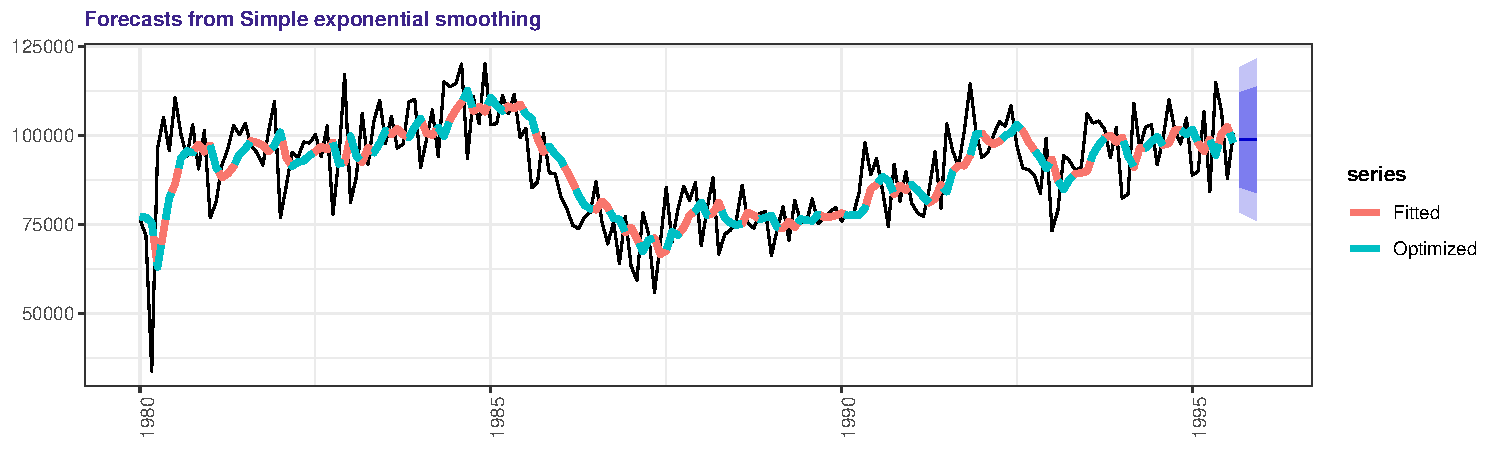
\includegraphics{homework-one_files/figure-latex/ha-7.3b3-1.pdf}

\hypertarget{assignment-five}{%
\chapter{Assignment Five}\label{assignment-five}}

\begin{itemize}
\tightlist
\item
  Hyndman 7.5
\item
  Hyndman 7.6
\item
  Hyndman 7.10
\end{itemize}

\begin{Shaded}
\begin{Highlighting}[]
\CommentTok{# Textbook Packages}
\KeywordTok{library}\NormalTok{(fpp2)}
\KeywordTok{library}\NormalTok{(AppliedPredictiveModeling)}
\KeywordTok{library}\NormalTok{(mlbench)}

\CommentTok{# Processing}
\KeywordTok{library}\NormalTok{(tidyverse)}

\CommentTok{# Graphing}
\KeywordTok{library}\NormalTok{(ggplot2)}
\KeywordTok{library}\NormalTok{(grid)}
\KeywordTok{library}\NormalTok{(gridExtra)}
\KeywordTok{library}\NormalTok{(lemon)}

\CommentTok{# Math}
\KeywordTok{library}\NormalTok{(caret)}
\KeywordTok{library}\NormalTok{(forecast)}
\KeywordTok{library}\NormalTok{(randomForest)}
\KeywordTok{library}\NormalTok{(seasonal)}
\KeywordTok{library}\NormalTok{(psych)}
\KeywordTok{library}\NormalTok{(corrplot)}

\CommentTok{# Formatting}
\KeywordTok{library}\NormalTok{(knitr)}
\KeywordTok{library}\NormalTok{(kableExtra)}
\KeywordTok{library}\NormalTok{(default)}
\end{Highlighting}
\end{Shaded}

\hypertarget{hyndman-7.5}{%
\section{Hyndman 7.5}\label{hyndman-7.5}}

\begin{quote}
Data set books contains the daily sales of paperback and hardcover books at the same store. The task is to forecast the next four days' sales for paperback and hardcover books.
\end{quote}

\hypertarget{a.-plot-the-series-and-discuss-the-main-features-of-the-data.}{%
\subsection{a. Plot the series and discuss the main features of the data.}\label{a.-plot-the-series-and-discuss-the-main-features-of-the-data.}}

\hypertarget{timeseries-plot}{%
\subsubsection{Timeseries Plot}\label{timeseries-plot}}

The \texttt{books} data shows an overall positive trend over the 30-day period for paperback and hardcover books. There is heavy fluctuation between days, suggesting seasonality within the time series. While paperbacks and hardcovers both have a similar range of unit sales, peaks and valleys are not well synchronized.

\begin{Shaded}
\begin{Highlighting}[]
\KeywordTok{autoplot}\NormalTok{(books, }\DataTypeTok{facet =} \OtherTok{TRUE}\NormalTok{) }\OperatorTok{+}\StringTok{ }\KeywordTok{labs}\NormalTok{(}\DataTypeTok{title =} \StringTok{"Daily Sales of Paperback and Hardcover Books"}\NormalTok{, }
  \DataTypeTok{x =} \StringTok{"Days"}\NormalTok{, }\DataTypeTok{y =} \StringTok{"Sales"}\NormalTok{) }\OperatorTok{+}\StringTok{ }\KeywordTok{theme_bw}\NormalTok{() }\OperatorTok{+}\StringTok{ }\KeywordTok{theme}\NormalTok{()}
\end{Highlighting}
\end{Shaded}

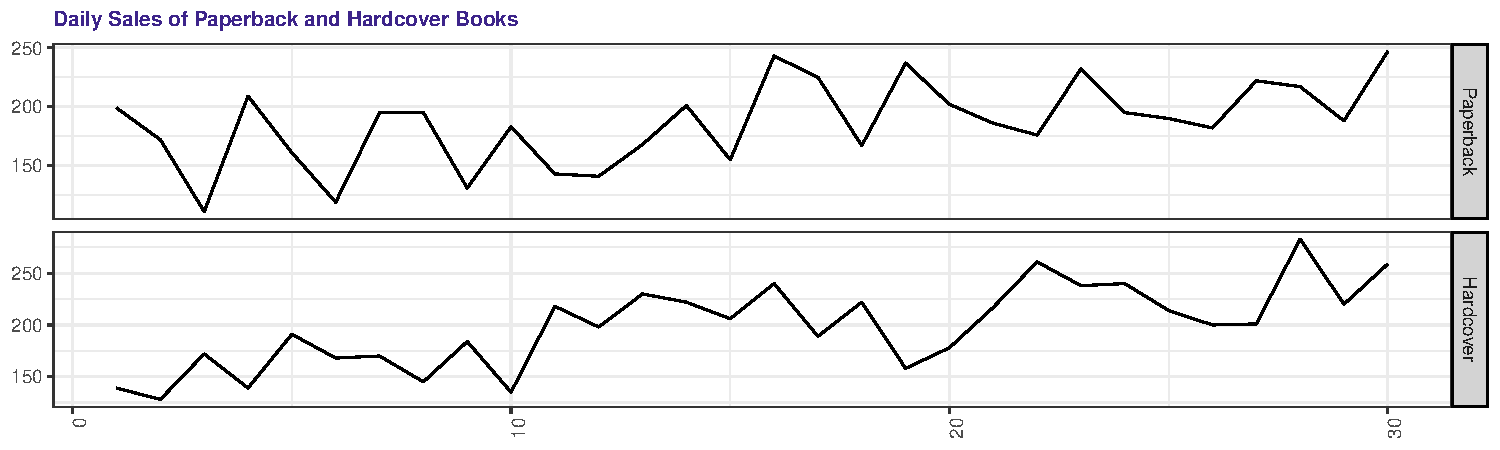
\includegraphics{homework-one_files/figure-latex/ha-7.5a1-1.pdf}

\hypertarget{decomposed-plot}{%
\subsubsection{Decomposed Plot}\label{decomposed-plot}}

We can look at the decomposed timeseries to better understand the trend and seasonality on a weekly basis. Sales tend to peak three times per week and increase throughout the entire month. The paperback books trend increases more drastically between weeks two and four, while hardcover books appear to have smoother incline. Hardcover books also show sharper fluctuations in the seasonal component.

\begin{Shaded}
\begin{Highlighting}[]
\NormalTok{paperback <-}\StringTok{ }\NormalTok{books[, }\DecValTok{1}\NormalTok{]}
\NormalTok{hardcover <-}\StringTok{ }\NormalTok{books[, }\DecValTok{2}\NormalTok{]}

\NormalTok{pb_plot <-}\StringTok{ }\KeywordTok{ts}\NormalTok{(paperback, }\DataTypeTok{frequency =} \DecValTok{7}\NormalTok{) }\OperatorTok\StringTok{ }\KeywordTok{decompose}\NormalTok{(}\DataTypeTok{type =} \StringTok{"multiplicative"}\NormalTok{) }\OperatorTok\StringTok{ }
\StringTok{  }\KeywordTok{autoplot}\NormalTok{() }\OperatorTok{+}\StringTok{ }\KeywordTok{labs}\NormalTok{(}\DataTypeTok{title =} \StringTok{"Paperback Books"}\NormalTok{, }\DataTypeTok{x =} \StringTok{"Weeks"}\NormalTok{) }\OperatorTok{+}\StringTok{ }
\StringTok{  }\KeywordTok{theme_bw}\NormalTok{() }\OperatorTok{+}\StringTok{ }\KeywordTok{theme}\NormalTok{()}

\NormalTok{hc_plot <-}\StringTok{ }\KeywordTok{ts}\NormalTok{(hardcover, }\DataTypeTok{frequency =} \DecValTok{7}\NormalTok{) }\OperatorTok\StringTok{ }\KeywordTok{decompose}\NormalTok{(}\DataTypeTok{type =} \StringTok{"multiplicative"}\NormalTok{) }\OperatorTok\StringTok{ }
\StringTok{  }\KeywordTok{autoplot}\NormalTok{() }\OperatorTok{+}\StringTok{ }\KeywordTok{labs}\NormalTok{(}\DataTypeTok{title =} \StringTok{"Hardcover Books"}\NormalTok{, }\DataTypeTok{x =} \StringTok{"Weeks"}\NormalTok{) }\OperatorTok{+}\StringTok{ }
\StringTok{  }\KeywordTok{theme_bw}\NormalTok{() }\OperatorTok{+}\StringTok{ }\KeywordTok{theme}\NormalTok{()}

\KeywordTok{grid.arrange}\NormalTok{(pb_plot, hc_plot, }\DataTypeTok{ncol =} \DecValTok{2}\NormalTok{, }\DataTypeTok{top =} \KeywordTok{textGrob}\NormalTok{(}\StringTok{"Decomposition of Multiplicative TS"}\NormalTok{, }
  \DataTypeTok{gp =} \KeywordTok{gpar}\NormalTok{(}\DataTypeTok{fontface =} \StringTok{"bold"}\NormalTok{, }\DataTypeTok{cex =} \FloatTok{1.5}\NormalTok{)))}
\end{Highlighting}
\end{Shaded}

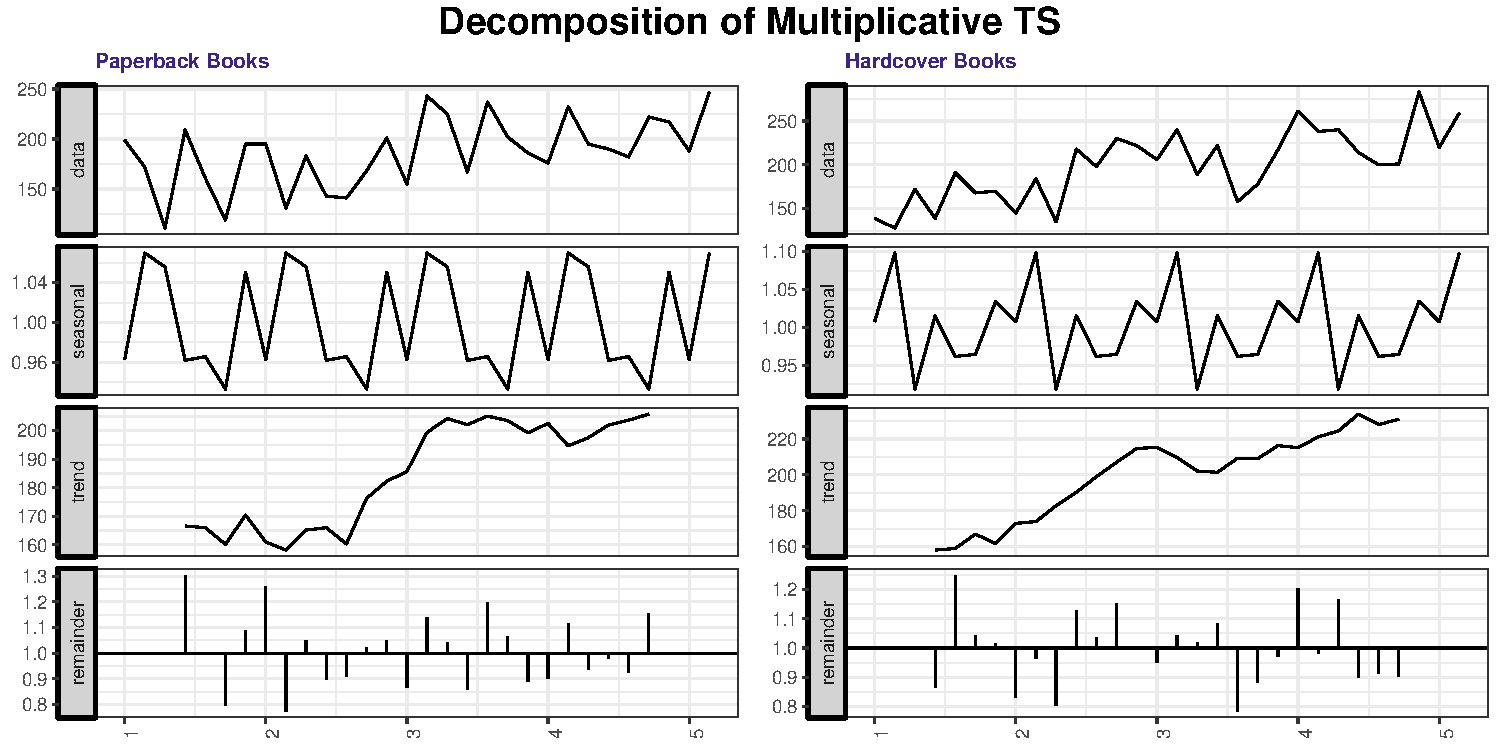
\includegraphics{homework-one_files/figure-latex/ha-7.5a2-1.pdf}

\hypertarget{b.-use-the-ses-function-to-forecast-each-series-and-plot-the-forecasts.}{%
\subsection{\texorpdfstring{b. Use the \texttt{ses()} function to forecast each series, and plot the forecasts.}{b. Use the ses() function to forecast each series, and plot the forecasts.}}\label{b.-use-the-ses-function-to-forecast-each-series-and-plot-the-forecasts.}}

\hypertarget{paperback-ses}{%
\subsubsection{Paperback SES}\label{paperback-ses}}

\begin{Shaded}
\begin{Highlighting}[]
\NormalTok{pb_ses <-}\StringTok{ }\KeywordTok{ses}\NormalTok{(paperback, }\DataTypeTok{h =} \DecValTok{4}\NormalTok{)}
\KeywordTok{summary}\NormalTok{(pb_ses)}
\end{Highlighting}
\end{Shaded}

\begin{verbatim}
FALSE 
FALSE Forecast method: Simple exponential smoothing
FALSE 
FALSE Model Information:
FALSE Simple exponential smoothing 
FALSE 
FALSE Call:
FALSE  ses(y = paperback, h = 4) 
FALSE 
FALSE   Smoothing parameters:
FALSE     alpha = 0.1685 
FALSE 
FALSE   Initial states:
FALSE     l = 170.8271 
FALSE 
FALSE   sigma:  34.8183
FALSE 
FALSE      AIC     AICc      BIC 
FALSE 318.9747 319.8978 323.1783 
FALSE 
FALSE Error measures:
FALSE                    ME     RMSE     MAE       MPE
FALSE Training set 7.175981 33.63769 27.8431 0.4736071
FALSE                  MAPE      MASE       ACF1
FALSE Training set 15.57784 0.7021303 -0.2117522
FALSE 
FALSE Forecasts:
FALSE    Point Forecast    Lo 80    Hi 80    Lo 95    Hi 95
FALSE 31       207.1097 162.4882 251.7311 138.8670 275.3523
FALSE 32       207.1097 161.8589 252.3604 137.9046 276.3147
FALSE 33       207.1097 161.2382 252.9811 136.9554 277.2639
FALSE 34       207.1097 160.6259 253.5935 136.0188 278.2005
\end{verbatim}

\hypertarget{hardcover-ses}{%
\subsubsection{Hardcover SES}\label{hardcover-ses}}

\begin{Shaded}
\begin{Highlighting}[]
\NormalTok{hc_ses <-}\StringTok{ }\KeywordTok{ses}\NormalTok{(hardcover, }\DataTypeTok{h =} \DecValTok{4}\NormalTok{)}
\KeywordTok{summary}\NormalTok{(hc_ses)}
\end{Highlighting}
\end{Shaded}

\begin{verbatim}
FALSE 
FALSE Forecast method: Simple exponential smoothing
FALSE 
FALSE Model Information:
FALSE Simple exponential smoothing 
FALSE 
FALSE Call:
FALSE  ses(y = hardcover, h = 4) 
FALSE 
FALSE   Smoothing parameters:
FALSE     alpha = 0.3283 
FALSE 
FALSE   Initial states:
FALSE     l = 149.2861 
FALSE 
FALSE   sigma:  33.0517
FALSE 
FALSE      AIC     AICc      BIC 
FALSE 315.8506 316.7737 320.0542 
FALSE 
FALSE Error measures:
FALSE                    ME     RMSE      MAE      MPE
FALSE Training set 9.166735 31.93101 26.77319 2.636189
FALSE                  MAPE      MASE       ACF1
FALSE Training set 13.39487 0.7987887 -0.1417763
FALSE 
FALSE Forecasts:
FALSE    Point Forecast    Lo 80    Hi 80    Lo 95    Hi 95
FALSE 31       239.5601 197.2026 281.9176 174.7799 304.3403
FALSE 32       239.5601 194.9788 284.1414 171.3788 307.7414
FALSE 33       239.5601 192.8607 286.2595 168.1396 310.9806
FALSE 34       239.5601 190.8347 288.2855 165.0410 314.0792
\end{verbatim}

\hypertarget{plot}{%
\subsubsection{Plot}\label{plot}}

\begin{Shaded}
\begin{Highlighting}[]
\NormalTok{pb_ses_plot <-}\StringTok{ }\KeywordTok{autoplot}\NormalTok{(pb_ses, }\DataTypeTok{size =} \DecValTok{1}\NormalTok{, }\DataTypeTok{fcol =} \StringTok{"#0044cc"}\NormalTok{) }\OperatorTok{+}\StringTok{ }
\StringTok{  }\KeywordTok{autolayer}\NormalTok{(}\KeywordTok{fitted}\NormalTok{(pb_ses), }\DataTypeTok{series =} \StringTok{"Fitted"}\NormalTok{, }\DataTypeTok{alpha =} \FloatTok{0.75}\NormalTok{, }
    \DataTypeTok{size =} \FloatTok{1.5}\NormalTok{, }\DataTypeTok{color =} \StringTok{"#99b3ff"}\NormalTok{) }\OperatorTok{+}\StringTok{ }\KeywordTok{labs}\NormalTok{(}\DataTypeTok{title =} \StringTok{"Paperback Books"}\NormalTok{, }
  \DataTypeTok{y =} \StringTok{"Sales"}\NormalTok{, }\DataTypeTok{x =} \StringTok{"Days"}\NormalTok{) }\OperatorTok{+}\StringTok{ }\KeywordTok{theme_bw}\NormalTok{() }\OperatorTok{+}\StringTok{ }\KeywordTok{theme}\NormalTok{()}

\NormalTok{hc_ses_plot <-}\StringTok{ }\KeywordTok{autoplot}\NormalTok{(hc_ses, }\DataTypeTok{size =} \DecValTok{1}\NormalTok{, }\DataTypeTok{fcol =} \StringTok{"#0044cc"}\NormalTok{) }\OperatorTok{+}\StringTok{ }
\StringTok{  }\KeywordTok{autolayer}\NormalTok{(}\KeywordTok{fitted}\NormalTok{(hc_ses), }\DataTypeTok{series =} \StringTok{"Fitted"}\NormalTok{, }\DataTypeTok{alpha =} \FloatTok{0.75}\NormalTok{, }
    \DataTypeTok{size =} \FloatTok{1.5}\NormalTok{, }\DataTypeTok{color =} \StringTok{"#99b3ff"}\NormalTok{) }\OperatorTok{+}\StringTok{ }\KeywordTok{labs}\NormalTok{(}\DataTypeTok{title =} \StringTok{"Hardcover Books"}\NormalTok{, }
  \DataTypeTok{y =} \StringTok{"Sales"}\NormalTok{, }\DataTypeTok{x =} \StringTok{"Days"}\NormalTok{) }\OperatorTok{+}\StringTok{ }\KeywordTok{theme_bw}\NormalTok{() }\OperatorTok{+}\StringTok{ }\KeywordTok{theme}\NormalTok{()}

\KeywordTok{grid.arrange}\NormalTok{(pb_ses_plot, hc_ses_plot, }\DataTypeTok{ncol =} \DecValTok{2}\NormalTok{, }\DataTypeTok{top =} \KeywordTok{textGrob}\NormalTok{(}\StringTok{"4-Day Forecast (SES)"}\NormalTok{, }
  \DataTypeTok{gp =} \KeywordTok{gpar}\NormalTok{(}\DataTypeTok{fontface =} \StringTok{"bold"}\NormalTok{, }\DataTypeTok{cex =} \FloatTok{1.5}\NormalTok{)))}
\end{Highlighting}
\end{Shaded}

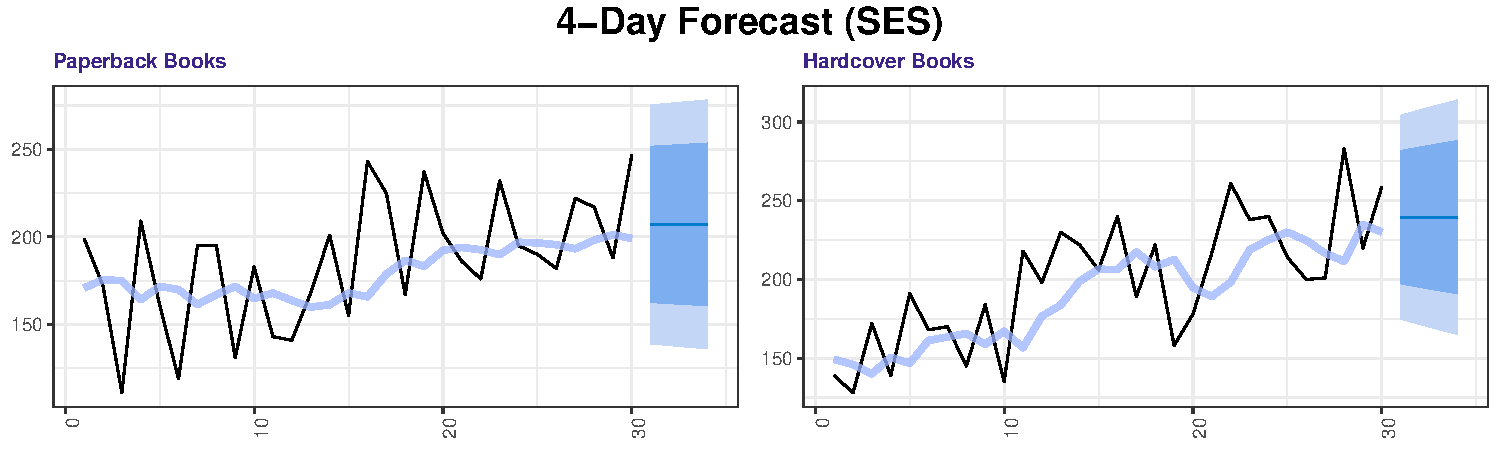
\includegraphics{homework-one_files/figure-latex/ha-7.5b3-1.pdf}

As SES may work well when their is no clear trend or seasonal pattern. As it generates the next probable value and uses that for all future forecasting values, however \texttt{ses()} may not be the best long-term forecasting model for this particular data.

\hypertarget{c.-compute-the-rmse-values-for-the-training-data-in-each-case.}{%
\subsection{c. Compute the RMSE values for the training data in each case.}\label{c.-compute-the-rmse-values-for-the-training-data-in-each-case.}}

The root mean squared error (RMSE) is calculated below and tells us the spread between the residual errors from our predicted and observed using the SES method. The RMSE for paperback books is slightly higher than hardcover, suggesting better accuracy in the later's predictions.

\begin{Shaded}
\begin{Highlighting}[]
\CommentTok{# manual calculation}
\KeywordTok{sqrt}\NormalTok{(}\KeywordTok{mean}\NormalTok{(pb_ses}\OperatorTok{$}\NormalTok{residuals}\OperatorTok{^}\DecValTok{2}\NormalTok{))}
\KeywordTok{sqrt}\NormalTok{(}\KeywordTok{mean}\NormalTok{(hc_ses}\OperatorTok{$}\NormalTok{residuals}\OperatorTok{^}\DecValTok{2}\NormalTok{))}

\CommentTok{# caret package}
\KeywordTok{RMSE}\NormalTok{(}\KeywordTok{fitted}\NormalTok{(pb_ses), paperback)}
\KeywordTok{RMSE}\NormalTok{(}\KeywordTok{fitted}\NormalTok{(hc_ses), hardcover)}
\end{Highlighting}
\end{Shaded}

\textbf{Paperback RMSE:} 33.6376868\\
\textbf{Hardcover RMSE:} 31.931015

\hypertarget{hyndman-7.6}{%
\section{Hyndman 7.6}\label{hyndman-7.6}}

\hypertarget{a.-now-apply-holts-linear-method-to-the-paperback-and-hardback-series-and-compute-four-day-forecasts-in-each-case.}{%
\subsection{a. Now apply Holt's linear method to the paperback and hardback series and compute four-day forecasts in each case.}\label{a.-now-apply-holts-linear-method-to-the-paperback-and-hardback-series-and-compute-four-day-forecasts-in-each-case.}}

\begin{Shaded}
\begin{Highlighting}[]
\NormalTok{hardcover <-}\StringTok{ }\KeywordTok{ts}\NormalTok{(books[, }\DecValTok{2}\NormalTok{], }\DataTypeTok{start =} \DecValTok{1}\NormalTok{, }\DataTypeTok{frequency =} \DecValTok{7}\NormalTok{)}
\NormalTok{softbound <-}\StringTok{ }\KeywordTok{ts}\NormalTok{(books[, }\DecValTok{1}\NormalTok{], }\DataTypeTok{start =} \DecValTok{1}\NormalTok{, }\DataTypeTok{frequency =} \DecValTok{7}\NormalTok{)}

\NormalTok{hb <-}\StringTok{ }\KeywordTok{ses}\NormalTok{(hardcover, }\DataTypeTok{h =} \DecValTok{5}\NormalTok{)}
\NormalTok{sb <-}\StringTok{ }\KeywordTok{ses}\NormalTok{(softbound, }\DataTypeTok{h =} \DecValTok{5}\NormalTok{)}

\NormalTok{acc_soft <-}\StringTok{ }\KeywordTok{accuracy}\NormalTok{(sb)}
\NormalTok{acc_hard <-}\StringTok{ }\KeywordTok{accuracy}\NormalTok{(hb)}

\NormalTok{holt_soft <-}\StringTok{ }\KeywordTok{holt}\NormalTok{(softbound, }\DataTypeTok{seasonal =} \StringTok{"additive"}\NormalTok{, }\DataTypeTok{h =} \DecValTok{4}\NormalTok{)}
\NormalTok{holt_hard <-}\StringTok{ }\KeywordTok{holt}\NormalTok{(hardcover, }\DataTypeTok{seasonal =} \StringTok{"additive"}\NormalTok{, }\DataTypeTok{h =} \DecValTok{4}\NormalTok{)}

\NormalTok{acc_holt_hard <-}\StringTok{ }\KeywordTok{accuracy}\NormalTok{(holt_hard)}
\NormalTok{acc_holt_soft <-}\StringTok{ }\KeywordTok{accuracy}\NormalTok{(holt_soft)}

\NormalTok{pb_holt_plot <-}\StringTok{ }\KeywordTok{autoplot}\NormalTok{(holt_soft, }\DataTypeTok{size =} \DecValTok{1}\NormalTok{, }\DataTypeTok{fcol =} \StringTok{"#7733ff"}\NormalTok{) }\OperatorTok{+}\StringTok{ }
\StringTok{  }\KeywordTok{autolayer}\NormalTok{(}\KeywordTok{fitted}\NormalTok{(holt_soft), }\DataTypeTok{series =} \StringTok{"Fitted"}\NormalTok{, }\DataTypeTok{alpha =} \FloatTok{0.75}\NormalTok{, }
    \DataTypeTok{size =} \FloatTok{1.5}\NormalTok{, }\DataTypeTok{color =} \StringTok{"#e0b3ff"}\NormalTok{) }\OperatorTok{+}\StringTok{ }\KeywordTok{labs}\NormalTok{(}\DataTypeTok{title =} \StringTok{"Paperback Books"}\NormalTok{, }
  \DataTypeTok{y =} \StringTok{"Sales"}\NormalTok{, }\DataTypeTok{x =} \StringTok{"Days"}\NormalTok{) }\OperatorTok{+}\StringTok{ }\KeywordTok{theme_bw}\NormalTok{() }\OperatorTok{+}\StringTok{ }\KeywordTok{theme}\NormalTok{()}

\NormalTok{hc_holt_plot <-}\StringTok{ }\KeywordTok{autoplot}\NormalTok{(holt_hard, }\DataTypeTok{size =} \DecValTok{1}\NormalTok{, }\DataTypeTok{fcol =} \StringTok{"#7733ff"}\NormalTok{) }\OperatorTok{+}\StringTok{ }
\StringTok{  }\KeywordTok{autolayer}\NormalTok{(}\KeywordTok{fitted}\NormalTok{(holt_hard), }\DataTypeTok{series =} \StringTok{"Fitted"}\NormalTok{, }\DataTypeTok{alpha =} \FloatTok{0.75}\NormalTok{, }
    \DataTypeTok{size =} \FloatTok{1.5}\NormalTok{, }\DataTypeTok{color =} \StringTok{"#e0b3ff"}\NormalTok{) }\OperatorTok{+}\StringTok{ }\KeywordTok{labs}\NormalTok{(}\DataTypeTok{title =} \StringTok{"Hardcover Books"}\NormalTok{, }
  \DataTypeTok{y =} \StringTok{"Sales"}\NormalTok{, }\DataTypeTok{x =} \StringTok{"Days"}\NormalTok{) }\OperatorTok{+}\StringTok{ }\KeywordTok{theme_bw}\NormalTok{() }\OperatorTok{+}\StringTok{ }\KeywordTok{theme}\NormalTok{()}

\KeywordTok{grid.arrange}\NormalTok{(pb_holt_plot, hc_holt_plot, }\DataTypeTok{ncol =} \DecValTok{2}\NormalTok{, }\DataTypeTok{top =} \KeywordTok{textGrob}\NormalTok{(}\StringTok{"4-Day Forecast (Holt)"}\NormalTok{, }
  \DataTypeTok{gp =} \KeywordTok{gpar}\NormalTok{(}\DataTypeTok{fontface =} \StringTok{"bold"}\NormalTok{, }\DataTypeTok{cex =} \FloatTok{1.5}\NormalTok{)))}
\end{Highlighting}
\end{Shaded}

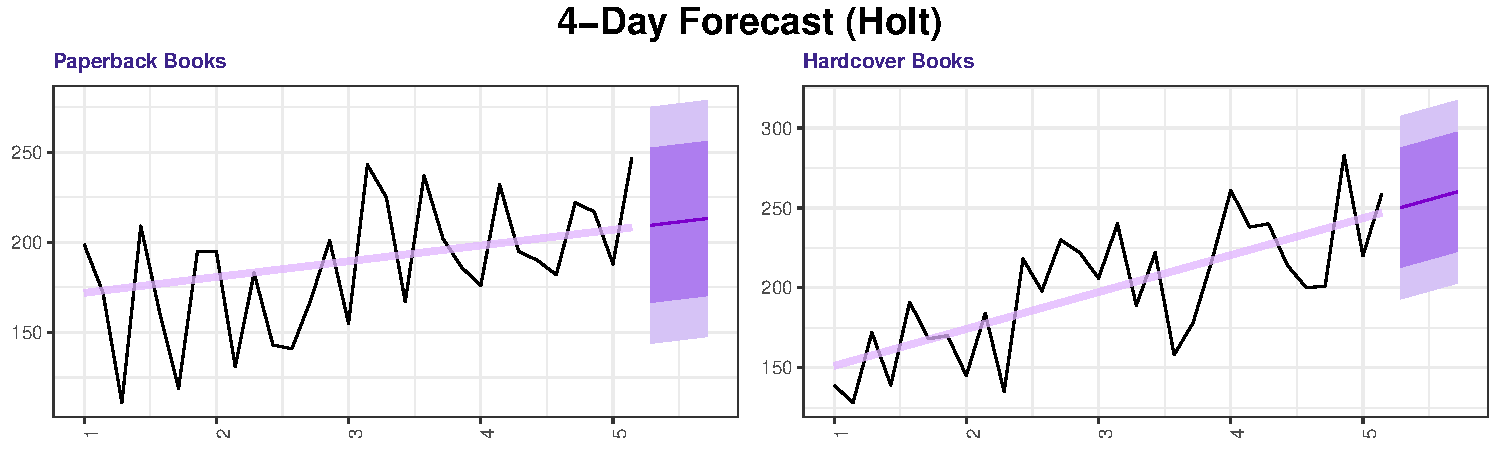
\includegraphics{homework-one_files/figure-latex/ha7.6a-1.pdf}

As would be expected, Holt's linear method generates a linear trend forecast.

\hypertarget{b.-compare-the-rmse-measures-of-holts-method-for-the-two-series-to-those-of-simple-exponential-smoothing-in-the-previous-question.-discuss-the-merits-of-the-two-forecasting-methods-for-these-data-sets.}{%
\subsection{b. Compare the RMSE measures of Holt's method for the two series to those of simple exponential smoothing in the previous question. Discuss the merits of the two forecasting methods for these data sets.}\label{b.-compare-the-rmse-measures-of-holts-method-for-the-two-series-to-those-of-simple-exponential-smoothing-in-the-previous-question.-discuss-the-merits-of-the-two-forecasting-methods-for-these-data-sets.}}

\begin{quote}
Remember that Holt's method is using one more parameter than SES.
\end{quote}

\textbf{RMSE Exponential Smoothed Hardcover Sales:} 31.931\\
\textbf{RMSE Exponential Smoothed Paperback Sales:} 33.638\\
\textbf{RMSE Holt-Winters Hardcover Sales:} 27.194\\
\textbf{RMSE Holt-Winters Paperback Sales:} 31.137

The Holt-Winter method does indeed reduce the root mean squared errors for both the paperback and hardcover book sales. This would suggest that there is in fact some level of trend acting on the book sales series.

\hypertarget{c.-compare-the-forecasts-for-the-two-series-using-both-methods.-which-do-you-think-is-best}{%
\subsection{c. Compare the forecasts for the two series using both methods. Which do you think is best?}\label{c.-compare-the-forecasts-for-the-two-series-using-both-methods.-which-do-you-think-is-best}}

\begin{Shaded}
\begin{Highlighting}[]
\NormalTok{fc_hh <-}\StringTok{ }\KeywordTok{forecast}\NormalTok{(holt_hard)}
\NormalTok{fc_sh <-}\StringTok{ }\KeywordTok{forecast}\NormalTok{(holt_soft)}

\NormalTok{fc_hes <-}\StringTok{ }\KeywordTok{forecast}\NormalTok{(hb, }\DataTypeTok{h =} \DecValTok{4}\NormalTok{)}
\NormalTok{fc_ses <-}\StringTok{ }\KeywordTok{forecast}\NormalTok{(sb, }\DataTypeTok{h =} \DecValTok{4}\NormalTok{)}

\NormalTok{p1 <-}\StringTok{ }\KeywordTok{autoplot}\NormalTok{(softbound) }\OperatorTok{+}\StringTok{ }\KeywordTok{autolayer}\NormalTok{(fc_ses, }\DataTypeTok{series =} \StringTok{"SES Paperback"}\NormalTok{, }
  \DataTypeTok{PI =} \OtherTok{FALSE}\NormalTok{) }\OperatorTok{+}\StringTok{ }\KeywordTok{autolayer}\NormalTok{(fc_sh, }\DataTypeTok{series =} \StringTok{"Holt Paperback"}\NormalTok{, }
  \DataTypeTok{PI =} \OtherTok{FALSE}\NormalTok{) }\OperatorTok{+}\StringTok{ }\KeywordTok{labs}\NormalTok{(}\DataTypeTok{title =} \StringTok{"Paperback Sales"}\NormalTok{, }\DataTypeTok{x =} \StringTok{"Year"}\NormalTok{, }
  \DataTypeTok{y =} \StringTok{"Daily Sales of Paperback Books"}\NormalTok{) }\OperatorTok{+}\StringTok{ }\KeywordTok{theme_bw}\NormalTok{() }\OperatorTok{+}\StringTok{ }
\StringTok{  }\KeywordTok{theme}\NormalTok{(}\DataTypeTok{legend.position =} \StringTok{"bottom"}\NormalTok{)}


\NormalTok{p2 <-}\StringTok{ }\KeywordTok{autoplot}\NormalTok{(hardcover) }\OperatorTok{+}\StringTok{ }\KeywordTok{autolayer}\NormalTok{(fc_hes, }\DataTypeTok{series =} \StringTok{"SES Paperback"}\NormalTok{, }
  \DataTypeTok{PI =} \OtherTok{FALSE}\NormalTok{) }\OperatorTok{+}\StringTok{ }\KeywordTok{autolayer}\NormalTok{(fc_hh, }\DataTypeTok{series =} \StringTok{"Holt Paperback"}\NormalTok{, }
  \DataTypeTok{PI =} \OtherTok{FALSE}\NormalTok{) }\OperatorTok{+}\StringTok{ }\KeywordTok{labs}\NormalTok{(}\DataTypeTok{title =} \StringTok{"Hardcover Sales"}\NormalTok{, }\DataTypeTok{x =} \StringTok{"Year"}\NormalTok{, }
  \DataTypeTok{y =} \StringTok{"Daily Sales of Hardcover Books"}\NormalTok{) }\OperatorTok{+}\StringTok{ }\KeywordTok{theme_bw}\NormalTok{() }\OperatorTok{+}\StringTok{ }
\StringTok{  }\KeywordTok{theme}\NormalTok{(}\DataTypeTok{legend.position =} \StringTok{"bottom"}\NormalTok{)}

\KeywordTok{grid.arrange}\NormalTok{(p1, p2, }\DataTypeTok{nrow =} \DecValTok{1}\NormalTok{, }\DataTypeTok{top =} \KeywordTok{textGrob}\NormalTok{(}\StringTok{"Methods Comparison"}\NormalTok{, }
  \DataTypeTok{gp =} \KeywordTok{gpar}\NormalTok{(}\DataTypeTok{fontface =} \StringTok{"bold"}\NormalTok{, }\DataTypeTok{cex =} \FloatTok{1.5}\NormalTok{)))}
\end{Highlighting}
\end{Shaded}

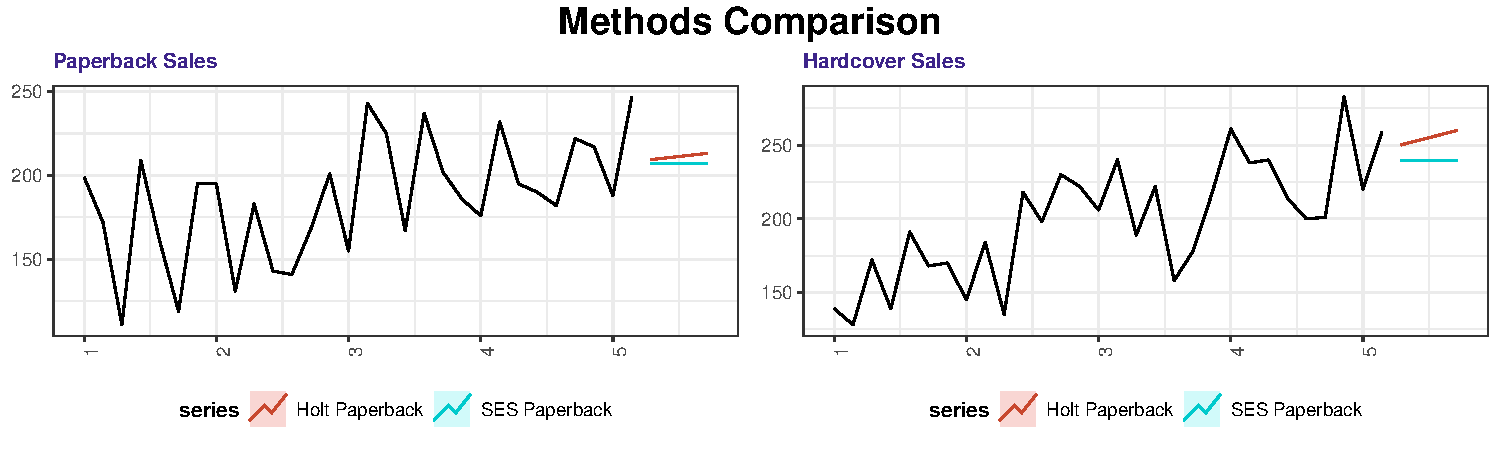
\includegraphics{homework-one_files/figure-latex/ha7.6c-1.pdf}

While Holt's method provided better accuracy measures (RMSE), it is a tough choice to pick one model over the other because neither is particularly robust over the long term. the SES is providing a continuous flat prediction which we can see is clearly not how the series has evolved in the past. On the other hand Holt's method does account for the trend but not the seasonality, so at some point it too would fail. Choosing a model from the two should be done based on your end need (ses being more conservative than holt's method) and with the understanding that more than a few observations forward and either of them will likely underperform.

\hypertarget{d.-calculate-a-95-prediction-interval-for-the-first-forecast-for-each-series-using-the-rmse-values-and-assuming-normal-errors.-compare-your-intervals-with-those-produced-using-ses-and-holt.}{%
\subsubsection{d. Calculate a 95\% prediction interval for the first forecast for each series, using the RMSE values and assuming normal errors. Compare your intervals with those produced using ses and holt.}\label{d.-calculate-a-95-prediction-interval-for-the-first-forecast-for-each-series-using-the-rmse-values-and-assuming-normal-errors.-compare-your-intervals-with-those-produced-using-ses-and-holt.}}

\begin{Shaded}
\begin{Highlighting}[]
\NormalTok{pi_ses_s <-}\StringTok{ }\FloatTok{1.96} \OperatorTok{*}\StringTok{ }\NormalTok{acc_soft[}\DecValTok{2}\NormalTok{]}
\NormalTok{pi_ses_h <-}\StringTok{ }\FloatTok{1.96} \OperatorTok{*}\StringTok{ }\NormalTok{acc_hard[}\DecValTok{2}\NormalTok{]}

\NormalTok{pi_hl_s <-}\StringTok{ }\FloatTok{1.96} \OperatorTok{*}\StringTok{ }\NormalTok{acc_holt_soft[}\DecValTok{2}\NormalTok{]}
\NormalTok{pi_hl_s <-}\StringTok{ }\FloatTok{1.96} \OperatorTok{*}\StringTok{ }\NormalTok{acc_holt_hard[}\DecValTok{2}\NormalTok{]}

\NormalTok{l_interval_ses_s <-}\StringTok{ }\KeywordTok{round}\NormalTok{(fc_ses}\OperatorTok{$}\NormalTok{mean[}\DecValTok{1}\NormalTok{] }\OperatorTok{-}\StringTok{ }\NormalTok{pi_ses_s, }\DecValTok{3}\NormalTok{)}
\NormalTok{l_interval_ses_h <-}\StringTok{ }\KeywordTok{round}\NormalTok{(fc_hes}\OperatorTok{$}\NormalTok{mean[}\DecValTok{1}\NormalTok{] }\OperatorTok{-}\StringTok{ }\NormalTok{pi_ses_h, }\DecValTok{3}\NormalTok{)}

\NormalTok{l_interval_hl_s <-}\StringTok{ }\KeywordTok{round}\NormalTok{(fc_sh}\OperatorTok{$}\NormalTok{mean[}\DecValTok{1}\NormalTok{] }\OperatorTok{-}\StringTok{ }\NormalTok{pi_hl_s, }\DecValTok{3}\NormalTok{)}
\NormalTok{l_interval_hl_h <-}\StringTok{ }\KeywordTok{round}\NormalTok{(fc_hh}\OperatorTok{$}\NormalTok{mean[}\DecValTok{1}\NormalTok{] }\OperatorTok{-}\StringTok{ }\NormalTok{pi_hl_s, }\DecValTok{3}\NormalTok{)}

\NormalTok{u_interval_ses_s <-}\StringTok{ }\KeywordTok{round}\NormalTok{(fc_ses}\OperatorTok{$}\NormalTok{mean[}\DecValTok{1}\NormalTok{] }\OperatorTok{+}\StringTok{ }\NormalTok{pi_ses_s, }\DecValTok{3}\NormalTok{)}
\NormalTok{u_interval_ses_h <-}\StringTok{ }\KeywordTok{round}\NormalTok{(fc_hes}\OperatorTok{$}\NormalTok{mean[}\DecValTok{1}\NormalTok{] }\OperatorTok{+}\StringTok{ }\NormalTok{pi_ses_h, }\DecValTok{3}\NormalTok{)}

\NormalTok{u_interval_hl_s <-}\StringTok{ }\KeywordTok{round}\NormalTok{(fc_sh}\OperatorTok{$}\NormalTok{mean[}\DecValTok{1}\NormalTok{] }\OperatorTok{+}\StringTok{ }\NormalTok{pi_hl_s, }\DecValTok{3}\NormalTok{)}
\NormalTok{u_interval_hl_h <-}\StringTok{ }\KeywordTok{round}\NormalTok{(fc_hh}\OperatorTok{$}\NormalTok{mean[}\DecValTok{1}\NormalTok{] }\OperatorTok{+}\StringTok{ }\NormalTok{pi_hl_s, }\DecValTok{3}\NormalTok{)}
\end{Highlighting}
\end{Shaded}

\begin{longtable}[]{@{}lllll@{}}
\toprule
& Model Lower & Model Upper & Calculated Lower & Calculated Upper\tabularnewline
\midrule
\endhead
SES Softbound & 138.867 & 275.352 & 141.18 & 273.04\tabularnewline
SES Hardbound & 174.78 & 304.34 & 176.975 & 302.145\tabularnewline
Holt Softbound & 143.913 & 275.021 & 156.167 & 262.766\tabularnewline
Holt Hardbound & 192.922 & 307.426 & 196.874 & 303.473\tabularnewline
\bottomrule
\end{longtable}

The manually calculated and library-generated prediction intervals are not exactly the same, but they are close. Manual intervals are a bit less consistent with the library computed interval values using the Holt's linear method than they are with exponentially smoothed (SES) version. Additionally, as SES entails a flat forecast with higher RMSE, its interval is slightly wider than that generated by Holt's linear method.

\hypertarget{hyndman-7.10}{%
\section{Hyndman 7.10}\label{hyndman-7.10}}

\begin{quote}
For this exercise use data set ukcars, the quarterly UK passenger vehicle production data from 1977Q1--2005Q1.
\end{quote}

\hypertarget{a.-plot-the-data-and-describe-the-main-features-of-the-series.}{%
\subsection{a. Plot the data and describe the main features of the series.}\label{a.-plot-the-data-and-describe-the-main-features-of-the-series.}}

\begin{Shaded}
\begin{Highlighting}[]
\NormalTok{ukcdata <-}\StringTok{ }\KeywordTok{window}\NormalTok{(ukcars, }\DataTypeTok{start =} \DecValTok{1977}\NormalTok{, }\DataTypeTok{end =} \DecValTok{2005}\NormalTok{)}
\KeywordTok{autoplot}\NormalTok{(ukcdata) }\OperatorTok{+}\StringTok{ }\KeywordTok{labs}\NormalTok{(}\DataTypeTok{title =} \StringTok{"Quarterly UK Passenger Vehicle Production Data"}\NormalTok{, }
  \DataTypeTok{y =} \StringTok{"Production"}\NormalTok{, }\DataTypeTok{x =} \StringTok{"Year"}\NormalTok{)}
\end{Highlighting}
\end{Shaded}

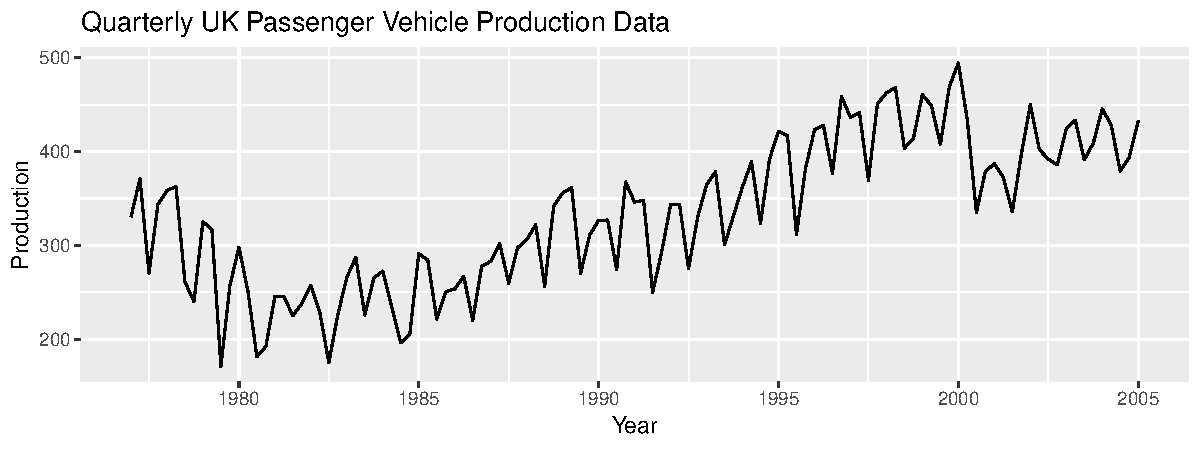
\includegraphics{homework-one_files/figure-latex/ha-7.10a-1.pdf}

There appears to be a general upward trend in production from 1982-Q3 to 2000-Q1. The overall time series shows fluxuations between years suggesting an underlying seasonality component. There also is some less structured periodicity and random-like variation.

\hypertarget{b.-decompose-the-series-using-stl-and-obtain-the-seasonally-adjusted-data.}{%
\subsection{b. Decompose the series using STL and obtain the seasonally adjusted data.}\label{b.-decompose-the-series-using-stl-and-obtain-the-seasonally-adjusted-data.}}

\hypertarget{stl-decomposition}{%
\subsection{STL Decomposition}\label{stl-decomposition}}

Through decomposition, we can confirm the overall increasing trend described in part (a). There are consistant seasonal fluxations which can we can futher evaluate using a seasonal plot.

\begin{Shaded}
\begin{Highlighting}[]
\NormalTok{ukc_stl <-}\StringTok{ }\KeywordTok{stl}\NormalTok{(ukcars, }\DataTypeTok{t.window =} \DecValTok{13}\NormalTok{, }\DataTypeTok{s.window =} \StringTok{"periodic"}\NormalTok{, }
  \DataTypeTok{robust =} \OtherTok{TRUE}\NormalTok{)}

\NormalTok{ukc_stl }\OperatorTok\StringTok{ }\KeywordTok{autoplot}\NormalTok{() }\OperatorTok{+}\StringTok{ }\KeywordTok{ggtitle}\NormalTok{(}\StringTok{"Decomposition of UK Cars usign 'STL' "}\NormalTok{) }\OperatorTok{+}\StringTok{ }
\StringTok{  }\KeywordTok{theme_bw}\NormalTok{() }\OperatorTok{+}\StringTok{ }\KeywordTok{theme}\NormalTok{()}
\end{Highlighting}
\end{Shaded}

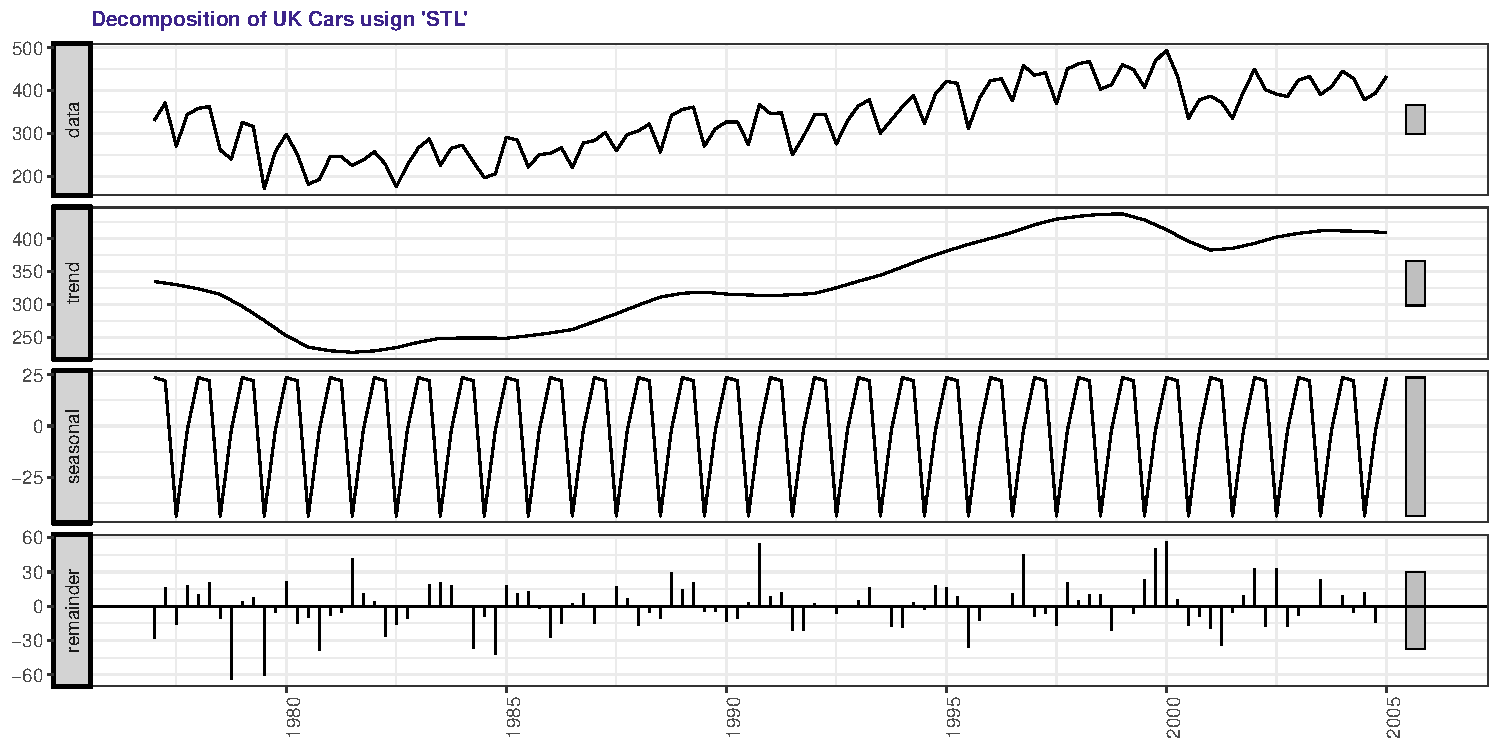
\includegraphics{homework-one_files/figure-latex/ha7.10b1-1.pdf}

\hypertarget{seasonal-plots}{%
\subsection{Seasonal Plots}\label{seasonal-plots}}

With the seasonal plot, we can see that our overal seasonality component increases between Q1-Q2, decreases Q2-Q3, and increases Q3-Q4. The intensity of the fluxuations vary by year. There are a few exceptions to this observation, for example, 2000 shows a two quarter decrease between Q1-Q3.

The subseries plot further confirms our seasonal pattern and shows that the smallest pattern changes occur between Q1-Q2. The decreases and increases between Q2-Q4 are much more distingushable.

\begin{Shaded}
\begin{Highlighting}[]
\NormalTok{ukc_s_plot <-}\StringTok{ }\KeywordTok{ggseasonplot}\NormalTok{(ukcdata, }\DataTypeTok{year.labels =} \OtherTok{TRUE}\NormalTok{, }\DataTypeTok{year.labels.left =}\NormalTok{ T, }
  \DataTypeTok{col =} \KeywordTok{rainbow}\NormalTok{(}\DecValTok{12}\NormalTok{, }\DataTypeTok{s =} \FloatTok{0.6}\NormalTok{, }\DataTypeTok{v =} \FloatTok{0.75}\NormalTok{)) }\OperatorTok{+}\StringTok{ }\KeywordTok{labs}\NormalTok{(}\DataTypeTok{title =} \StringTok{"Seasonal plot"}\NormalTok{, }
  \DataTypeTok{y =} \StringTok{"Production"}\NormalTok{) }\OperatorTok{+}\StringTok{ }\KeywordTok{theme_bw}\NormalTok{() }\OperatorTok{+}\StringTok{ }\KeywordTok{theme}\NormalTok{()}

\NormalTok{ukc_ss_plot <-}\StringTok{ }\KeywordTok{ggsubseriesplot}\NormalTok{(ukcdata) }\OperatorTok{+}\StringTok{ }\KeywordTok{labs}\NormalTok{(}\DataTypeTok{title =} \StringTok{"Subseries plot"}\NormalTok{, }
  \DataTypeTok{y =} \StringTok{"Production"}\NormalTok{) }\OperatorTok{+}\StringTok{ }\KeywordTok{theme_bw}\NormalTok{() }\OperatorTok{+}\StringTok{ }\KeywordTok{theme}\NormalTok{()}

\KeywordTok{grid.arrange}\NormalTok{(ukc_s_plot, ukc_ss_plot, }\DataTypeTok{ncol =} \DecValTok{2}\NormalTok{, }\DataTypeTok{top =} \StringTok{"Quarterly UK Passenger Vehicle Production Data"}\NormalTok{)}
\end{Highlighting}
\end{Shaded}

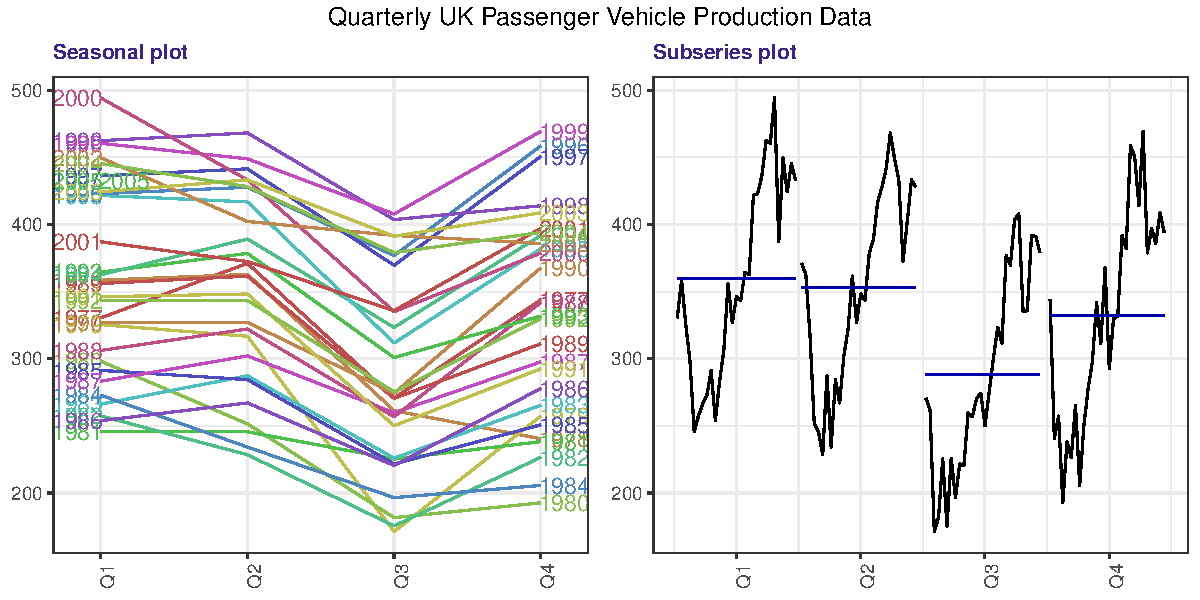
\includegraphics{homework-one_files/figure-latex/ha-7.10b2-1.pdf}

We can capture the seasonal component observed in the data and control for the changes overtime using a seasonal adjustment. We compared the seasonally adjusted data to the observed data for \texttt{ukcars} below:

\begin{Shaded}
\begin{Highlighting}[]
\NormalTok{ukc_seas <-}\StringTok{ }\KeywordTok{seasadj}\NormalTok{(ukc_stl)}

\KeywordTok{autoplot}\NormalTok{(ukcdata, }\DataTypeTok{series =} \StringTok{"Data"}\NormalTok{) }\OperatorTok{+}\StringTok{ }\KeywordTok{autolayer}\NormalTok{(ukc_seas, }
  \DataTypeTok{series =} \StringTok{"Seasonally Adjusted"}\NormalTok{) }\OperatorTok{+}\StringTok{ }\KeywordTok{labs}\NormalTok{(}\DataTypeTok{title =} \StringTok{"Quarterly UK Passenger Vehicle Production Data"}\NormalTok{, }
  \DataTypeTok{subtitle =} \StringTok{"Seasonally Adjusted Comparison"}\NormalTok{, }\DataTypeTok{x =} \StringTok{"Year"}\NormalTok{, }
  \DataTypeTok{y =} \StringTok{"Production"}\NormalTok{) }\OperatorTok{+}\StringTok{ }\KeywordTok{scale_colour_manual}\NormalTok{(}\DataTypeTok{values =} \KeywordTok{c}\NormalTok{(}\StringTok{"#bfbfbf"}\NormalTok{, }
  \StringTok{"#99b3ff"}\NormalTok{), }\DataTypeTok{breaks =} \KeywordTok{c}\NormalTok{(}\StringTok{"Data"}\NormalTok{, }\StringTok{"Seasonally Adjusted"}\NormalTok{, }
  \StringTok{"Trend"}\NormalTok{)) }\OperatorTok{+}\StringTok{ }\KeywordTok{theme_bw}\NormalTok{() }\OperatorTok{+}\StringTok{ }\KeywordTok{theme}\NormalTok{(}\DataTypeTok{legend.position =} \StringTok{"bottom"}\NormalTok{)}
\end{Highlighting}
\end{Shaded}

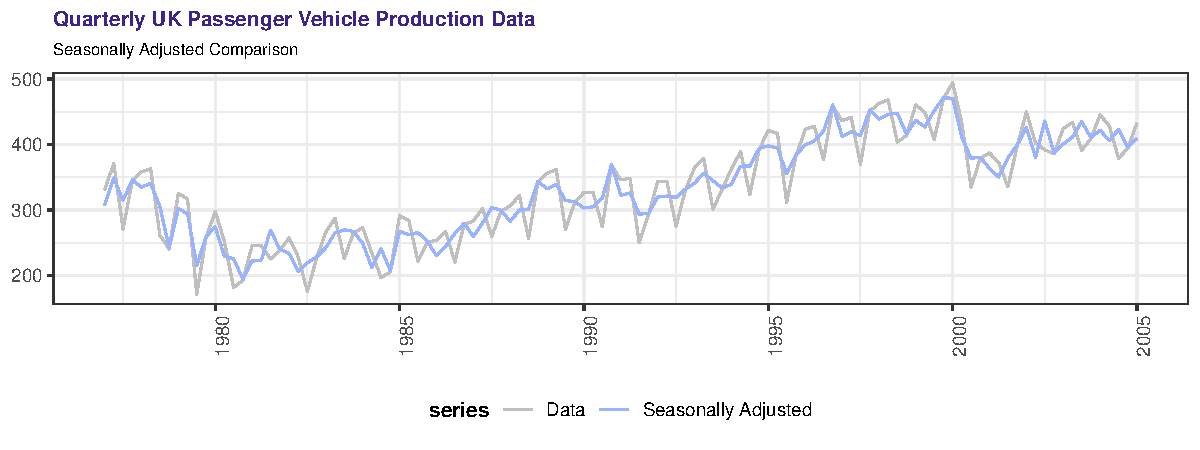
\includegraphics{homework-one_files/figure-latex/ha-7.10b3-1.pdf}

\hypertarget{c.-forecast-the-next-two-years-of-the-series-using-an-additive-damped-trend-method-applied-to-the-seasonally-adjusted-data.-this-can-be-done-in-one-step-using-stlf-with-arguments-etsmodelaan-dampedtrue.}{%
\subsection{c. Forecast the next two years of the series using an additive damped trend method applied to the seasonally adjusted data. (This can be done in one step using stlf() with arguments etsmodel=``AAN'', damped=TRUE.)}\label{c.-forecast-the-next-two-years-of-the-series-using-an-additive-damped-trend-method-applied-to-the-seasonally-adjusted-data.-this-can-be-done-in-one-step-using-stlf-with-arguments-etsmodelaan-dampedtrue.}}

As the data is seasonally adjusted, we use an AAN model (error = A, trend = A, and seasonal = N). Damped models are often better at forecasting long-run values.

\hypertarget{forecast}{%
\subsubsection{Forecast}\label{forecast}}

\begin{Shaded}
\begin{Highlighting}[]
\NormalTok{ukc_stlf1 <-}\StringTok{ }\KeywordTok{stlf}\NormalTok{(ukcdata, }\DataTypeTok{s.window =} \StringTok{"periodic"}\NormalTok{, }\DataTypeTok{etsmodel =} \StringTok{"AAN"}\NormalTok{, }
  \DataTypeTok{damped =} \OtherTok{TRUE}\NormalTok{, }\DataTypeTok{h =} \DecValTok{8}\NormalTok{)}
\NormalTok{rmse_holt_d <-}\StringTok{ }\KeywordTok{accuracy}\NormalTok{(ukc_stlf1)[}\DecValTok{2}\NormalTok{]}

\KeywordTok{kable}\NormalTok{(}\KeywordTok{forecast}\NormalTok{(ukc_stlf1), }\StringTok{"latex"}\NormalTok{) }\OperatorTok\StringTok{ }\KeywordTok{kable_styling}\NormalTok{(}\DataTypeTok{latex_options =} \KeywordTok{c}\NormalTok{(}\StringTok{"hold_position"}\NormalTok{, }
  \StringTok{"striped"}\NormalTok{))}
\end{Highlighting}
\end{Shaded}

\begingroup\fontsize{10}{12}\selectfont

\begin{tabu} to \linewidth {>{\raggedright}X>{\raggedleft}X>{\raggedleft}X>{\raggedleft}X>{\raggedleft}X>{\raggedleft}X}
\hline
  & Point Forecast & Lo 80 & Hi 80 & Lo 95 & Hi 95\\
\hline
\rowcolor{gray!6}  2005 Q2 & 406.4679 & 373.4863 & 439.4495 & 356.0269 & 456.9089\\
\hline
2005 Q3 & 406.4673 & 368.4766 & 444.4580 & 348.3655 & 464.5691\\
\hline
\rowcolor{gray!6}  2005 Q4 & 406.4668 & 364.0533 & 448.8804 & 341.6009 & 471.3327\\
\hline
2006 Q1 & 406.4664 & 360.0485 & 452.8842 & 335.4764 & 477.4563\\
\hline
\rowcolor{gray!6}  2006 Q2 & 406.4660 & 356.3620 & 456.5700 & 329.8385 & 483.0934\\
\hline
2006 Q3 & 406.4656 & 352.9279 & 460.0033 & 324.5867 & 488.3444\\
\hline
\rowcolor{gray!6}  2006 Q4 & 406.4652 & 349.7005 & 463.2299 & 319.6511 & 493.2794\\
\hline
2007 Q1 & 406.4649 & 346.6465 & 466.2834 & 314.9805 & 497.9493\\
\hline
\end{tabu}
\endgroup{}

\hypertarget{plot-1}{%
\subsubsection{Plot}\label{plot-1}}

\begin{Shaded}
\begin{Highlighting}[]
\KeywordTok{autoplot}\NormalTok{(ukc_stlf1, }\DataTypeTok{size =} \FloatTok{1.25}\NormalTok{, }\DataTypeTok{fcol =} \StringTok{"#0044cc"}\NormalTok{) }\OperatorTok{+}\StringTok{ }\KeywordTok{autolayer}\NormalTok{(}\KeywordTok{fitted}\NormalTok{(ukc_stlf1), }
  \DataTypeTok{series =} \StringTok{"Fitted"}\NormalTok{, }\DataTypeTok{alpha =} \FloatTok{0.5}\NormalTok{, }\DataTypeTok{size =} \FloatTok{1.5}\NormalTok{, }\DataTypeTok{color =} \StringTok{"#99b3ff"}\NormalTok{) }\OperatorTok{+}\StringTok{ }
\StringTok{  }\KeywordTok{labs}\NormalTok{(}\DataTypeTok{y =} \StringTok{"Production"}\NormalTok{, }\DataTypeTok{x =} \StringTok{"Years"}\NormalTok{) }\OperatorTok{+}\StringTok{ }\KeywordTok{theme_bw}\NormalTok{() }\OperatorTok{+}\StringTok{ }\KeywordTok{theme}\NormalTok{()}
\end{Highlighting}
\end{Shaded}

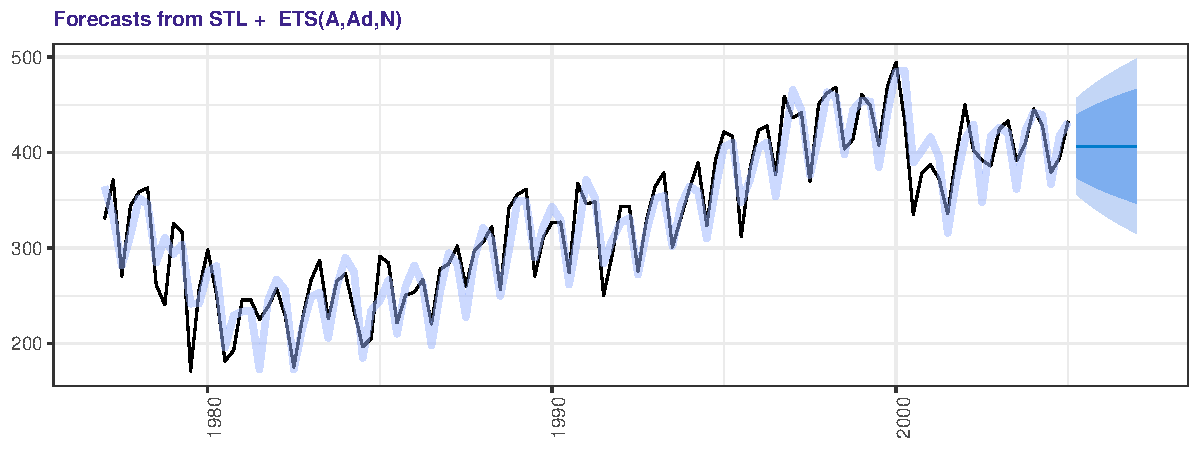
\includegraphics{homework-one_files/figure-latex/ha-7.10c2-1.pdf}

\hypertarget{d.-forecast-the-next-two-years-of-the-series-using-holts-linear-method-applied-to-the-seasonally-adjusted-data-as-before-but-with-dampedfalse.}{%
\subsection{d. Forecast the next two years of the series using Holt's linear method applied to the seasonally adjusted data (as before but with damped=FALSE).}\label{d.-forecast-the-next-two-years-of-the-series-using-holts-linear-method-applied-to-the-seasonally-adjusted-data-as-before-but-with-dampedfalse.}}

We again use an AAN model (error = A, trend = A, seasonality = N) - this time without damping, so point forecasts are a little bit higher.

\hypertarget{forecast-1}{%
\subsubsection{Forecast}\label{forecast-1}}

\begin{Shaded}
\begin{Highlighting}[]
\NormalTok{ukc_stlf2 <-}\StringTok{ }\KeywordTok{stlf}\NormalTok{(ukcdata, }\DataTypeTok{s.window =} \StringTok{"periodic"}\NormalTok{, }\DataTypeTok{etsmodel =} \StringTok{"AAN"}\NormalTok{, }
  \DataTypeTok{damped =} \OtherTok{FALSE}\NormalTok{, }\DataTypeTok{h =} \DecValTok{8}\NormalTok{)}
\NormalTok{rmse_holt_u <-}\StringTok{ }\KeywordTok{accuracy}\NormalTok{(ukc_stlf2)[}\DecValTok{2}\NormalTok{]}

\KeywordTok{kable}\NormalTok{(}\KeywordTok{forecast}\NormalTok{(ukc_stlf2), }\StringTok{"latex"}\NormalTok{) }\OperatorTok\StringTok{ }\KeywordTok{kable_styling}\NormalTok{(}\DataTypeTok{latex_options =} \KeywordTok{c}\NormalTok{(}\StringTok{"hold_position"}\NormalTok{, }
  \StringTok{"striped"}\NormalTok{))}
\end{Highlighting}
\end{Shaded}

\begingroup\fontsize{10}{12}\selectfont

\begin{tabu} to \linewidth {>{\raggedright}X>{\raggedleft}X>{\raggedleft}X>{\raggedleft}X>{\raggedleft}X>{\raggedleft}X}
\hline
  & Point Forecast & Lo 80 & Hi 80 & Lo 95 & Hi 95\\
\hline
\rowcolor{gray!6}  2005 Q2 & 407.6326 & 374.6715 & 440.5938 & 357.2229 & 458.0424\\
\hline
2005 Q3 & 408.4644 & 369.9399 & 446.9889 & 349.5463 & 467.3825\\
\hline
\rowcolor{gray!6}  2005 Q4 & 409.2962 & 365.9146 & 452.6778 & 342.9497 & 475.6426\\
\hline
2006 Q1 & 410.1280 & 362.3794 & 457.8765 & 337.1029 & 483.1531\\
\hline
\rowcolor{gray!6}  2006 Q2 & 410.9598 & 359.2102 & 462.7093 & 331.8157 & 490.1039\\
\hline
2006 Q3 & 411.7915 & 356.3277 & 467.2554 & 326.9669 & 496.6162\\
\hline
\rowcolor{gray!6}  2006 Q4 & 412.6233 & 353.6776 & 471.5690 & 322.4737 & 502.7730\\
\hline
2007 Q1 & 413.4551 & 351.2210 & 475.6892 & 318.2763 & 508.6339\\
\hline
\end{tabu}
\endgroup{}

\hypertarget{plot-2}{%
\subsubsection{Plot}\label{plot-2}}

\begin{Shaded}
\begin{Highlighting}[]
\KeywordTok{autoplot}\NormalTok{(ukc_stlf2, }\DataTypeTok{size =} \FloatTok{1.25}\NormalTok{, }\DataTypeTok{fcol =} \StringTok{"#0044cc"}\NormalTok{) }\OperatorTok{+}\StringTok{ }\KeywordTok{autolayer}\NormalTok{(}\KeywordTok{fitted}\NormalTok{(ukc_stlf2), }
  \DataTypeTok{series =} \StringTok{"Fitted"}\NormalTok{, }\DataTypeTok{alpha =} \FloatTok{0.5}\NormalTok{, }\DataTypeTok{size =} \FloatTok{1.5}\NormalTok{, }\DataTypeTok{color =} \StringTok{"#99b3ff"}\NormalTok{) }\OperatorTok{+}\StringTok{ }
\StringTok{  }\KeywordTok{labs}\NormalTok{(}\DataTypeTok{y =} \StringTok{"Production"}\NormalTok{, }\DataTypeTok{x =} \StringTok{"Years"}\NormalTok{) }\OperatorTok{+}\StringTok{ }\KeywordTok{theme_bw}\NormalTok{() }\OperatorTok{+}\StringTok{ }\KeywordTok{theme}\NormalTok{()}
\end{Highlighting}
\end{Shaded}

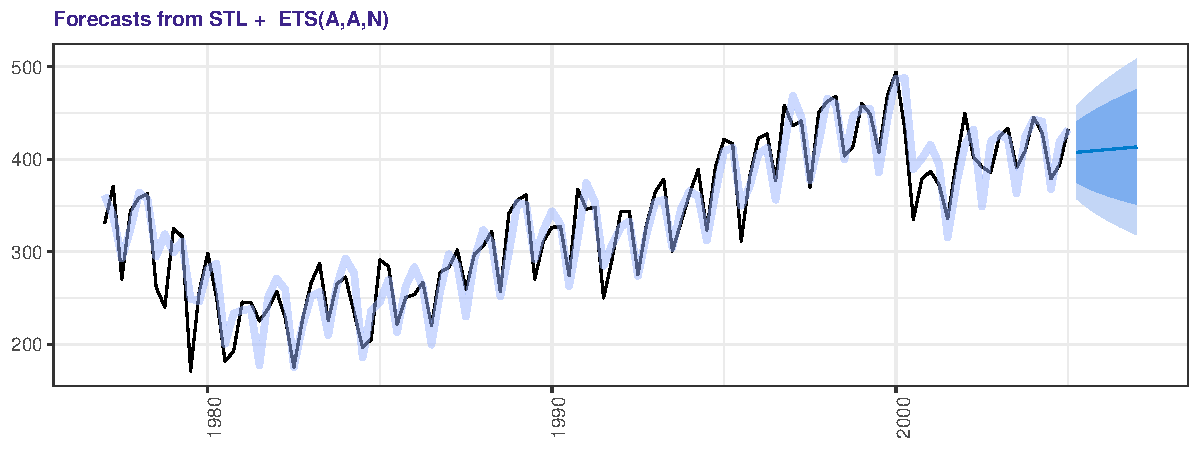
\includegraphics{homework-one_files/figure-latex/ha-7.10d2-1.pdf}

\hypertarget{e.-now-use-ets-to-choose-a-seasonal-model-for-the-data.}{%
\subsection{e. Now use ets() to choose a seasonal model for the data.}\label{e.-now-use-ets-to-choose-a-seasonal-model-for-the-data.}}

ETS automatically chooses the best model by minimizing AIC, which results in a error = A, trend = N, seasonal = A model.

\hypertarget{seasonal-model}{%
\subsubsection{Seasonal Model}\label{seasonal-model}}

\begin{Shaded}
\begin{Highlighting}[]
\NormalTok{ukc_ets <-}\StringTok{ }\KeywordTok{ets}\NormalTok{(ukcdata)}
\KeywordTok{summary}\NormalTok{(ukc_ets)}
\end{Highlighting}
\end{Shaded}

\begin{verbatim}
FALSE ETS(A,N,A) 
FALSE 
FALSE Call:
FALSE  ets(y = ukcdata) 
FALSE 
FALSE   Smoothing parameters:
FALSE     alpha = 0.6199 
FALSE     gamma = 1e-04 
FALSE 
FALSE   Initial states:
FALSE     l = 314.2568 
FALSE     s = -1.7579 -44.9601 21.1956 25.5223
FALSE 
FALSE   sigma:  25.9302
FALSE 
FALSE      AIC     AICc      BIC 
FALSE 1277.752 1278.819 1296.844 
FALSE 
FALSE Training set error measures:
FALSE                    ME     RMSE      MAE        MPE
FALSE Training set 1.313884 25.23244 20.17907 -0.1570979
FALSE                  MAPE      MASE       ACF1
FALSE Training set 6.629003 0.6576259 0.02573334
\end{verbatim}

\begin{Shaded}
\begin{Highlighting}[]
\NormalTok{ukc_ets_fc <-}\StringTok{ }\NormalTok{ukc_ets }\OperatorTok\StringTok{ }\KeywordTok{forecast}\NormalTok{(}\DataTypeTok{h =} \DecValTok{8}\NormalTok{)}
\NormalTok{rmse_ets <-}\StringTok{ }\KeywordTok{accuracy}\NormalTok{(ukc_ets)[}\DecValTok{2}\NormalTok{]}
\end{Highlighting}
\end{Shaded}

\hypertarget{forecast-2}{%
\subsubsection{Forecast}\label{forecast-2}}

\begin{Shaded}
\begin{Highlighting}[]
\KeywordTok{kable}\NormalTok{(ukc_ets_fc, }\StringTok{"latex"}\NormalTok{) }\OperatorTok\StringTok{ }\KeywordTok{kable_styling}\NormalTok{(}\DataTypeTok{latex_options =} \KeywordTok{c}\NormalTok{(}\StringTok{"hold_position"}\NormalTok{, }
  \StringTok{"striped"}\NormalTok{))}
\end{Highlighting}
\end{Shaded}

\begingroup\fontsize{10}{12}\selectfont

\begin{tabu} to \linewidth {>{\raggedright}X>{\raggedleft}X>{\raggedleft}X>{\raggedleft}X>{\raggedleft}X>{\raggedleft}X}
\hline
  & Point Forecast & Lo 80 & Hi 80 & Lo 95 & Hi 95\\
\hline
\rowcolor{gray!6}  2005 Q2 & 427.4885 & 394.2576 & 460.7195 & 376.6662 & 478.3109\\
\hline
2005 Q3 & 361.3329 & 322.2353 & 400.4305 & 301.5383 & 421.1275\\
\hline
\rowcolor{gray!6}  2005 Q4 & 404.5358 & 360.3437 & 448.7280 & 336.9497 & 472.1219\\
\hline
2006 Q1 & 431.8154 & 383.0568 & 480.5741 & 357.2455 & 506.3854\\
\hline
\rowcolor{gray!6}  2006 Q2 & 427.4885 & 374.5571 & 480.4200 & 346.5369 & 508.4401\\
\hline
2006 Q3 & 361.3329 & 304.5345 & 418.1313 & 274.4672 & 448.1986\\
\hline
\rowcolor{gray!6}  2006 Q4 & 404.5358 & 344.1174 & 464.9542 & 312.1338 & 496.9378\\
\hline
2007 Q1 & 431.8154 & 367.9809 & 495.6500 & 334.1890 & 529.4419\\
\hline
\end{tabu}
\endgroup{}

\hypertarget{plot-3}{%
\subsubsection{Plot}\label{plot-3}}

\begin{Shaded}
\begin{Highlighting}[]
\KeywordTok{autoplot}\NormalTok{(ukc_ets_fc, }\DataTypeTok{size =} \FloatTok{1.25}\NormalTok{, }\DataTypeTok{fcol =} \StringTok{"#0044cc"}\NormalTok{) }\OperatorTok{+}\StringTok{ }\KeywordTok{autolayer}\NormalTok{(}\KeywordTok{fitted}\NormalTok{(ukc_ets), }
  \DataTypeTok{series =} \StringTok{"Fitted"}\NormalTok{, }\DataTypeTok{alpha =} \FloatTok{0.5}\NormalTok{, }\DataTypeTok{size =} \FloatTok{1.5}\NormalTok{, }\DataTypeTok{color =} \StringTok{"#99b3ff"}\NormalTok{) }\OperatorTok{+}\StringTok{ }
\StringTok{  }\KeywordTok{labs}\NormalTok{(}\DataTypeTok{y =} \StringTok{"Production"}\NormalTok{, }\DataTypeTok{x =} \StringTok{"Years"}\NormalTok{)}
\end{Highlighting}
\end{Shaded}

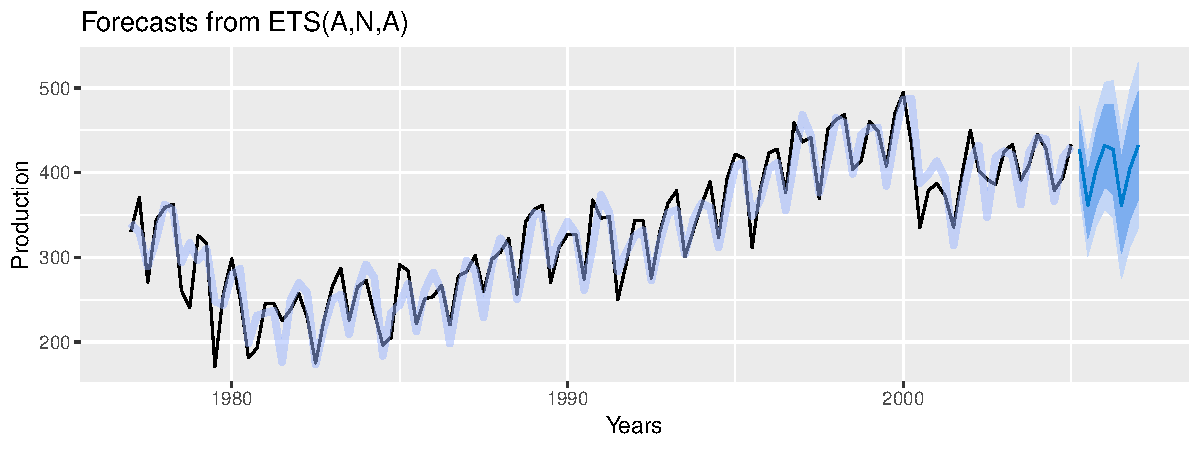
\includegraphics{homework-one_files/figure-latex/ha-7.10e2-1.pdf}

\hypertarget{f.-compare-the-rmse-of-the-ets-model-with-the-rmse-of-the-models-you-obtained-using-stl-decompositions.-which-gives-the-better-in-sample-fits}{%
\subsection{f. Compare the RMSE of the ETS model with the RMSE of the models you obtained using STL decompositions. Which gives the better in-sample fits?}\label{f.-compare-the-rmse-of-the-ets-model-with-the-rmse-of-the-models-you-obtained-using-stl-decompositions.-which-gives-the-better-in-sample-fits}}

Our STL decomponsition, using additive damped trend method with no seasonal components (\(A, A_d, N\)), produced the best in-sample fit. This model provided us with the lowest RMSE, suggesting the highest degree of accuracy between our predicted and observed data. We should note, however, there is a very small variation in RMSE between all STL and ETS models.

\begin{itemize}
\tightlist
\item
  \textbf{STL:} 25.2604123
\item
  \textbf{HOLT:} 25.1598573
\item
  \textbf{ETS:} 25.2324409
\end{itemize}

\hypertarget{g.-compare-the-forecasts-from-the-three-approaches-which-seems-most-reasonable}{%
\subsection{g. Compare the forecasts from the three approaches? Which seems most reasonable?}\label{g.-compare-the-forecasts-from-the-three-approaches-which-seems-most-reasonable}}

The forecasts from the ETS (\(A, N, A\)) model appears most reasonable and fits our data best. This is not surprising as the \texttt{ets} function automatically selects the methodology based on the provided data. The forecasts using STL were both linear, whereas the ETS model was able to predict seasonal pattern changes across our 2-year (8-quarter) prediction.

\begin{Shaded}
\begin{Highlighting}[]
\NormalTok{ukc_series <-}\StringTok{ }\KeywordTok{cbind}\NormalTok{(}\DataTypeTok{Data =}\NormalTok{ ukcdata, }\StringTok{`}\DataTypeTok{Forecast (STL1)}\StringTok{`}\NormalTok{ =}\StringTok{ }\NormalTok{ukc_stlf1[[}\StringTok{"mean"}\NormalTok{]], }
  \StringTok{`}\DataTypeTok{Forecast (STL2)}\StringTok{`}\NormalTok{ =}\StringTok{ }\NormalTok{ukc_stlf2[[}\StringTok{"mean"}\NormalTok{]], }\StringTok{`}\DataTypeTok{Forecast (ETS)}\StringTok{`}\NormalTok{ =}\StringTok{ }\NormalTok{ukc_ets_fc[[}\StringTok{"mean"}\NormalTok{]])}

\KeywordTok{autoplot}\NormalTok{(ukc_series, }\DataTypeTok{size =} \DecValTok{1}\NormalTok{, }\DataTypeTok{alpha =} \FloatTok{0.75}\NormalTok{) }\OperatorTok{+}\StringTok{ }\KeywordTok{scale_color_manual}\NormalTok{(}\DataTypeTok{name =} \StringTok{""}\NormalTok{, }
  \DataTypeTok{values =} \KeywordTok{c}\NormalTok{(}\StringTok{"#000000"}\NormalTok{, }\StringTok{"#0044cc"}\NormalTok{, }\StringTok{"#99b3ff"}\NormalTok{, }\StringTok{"#e0b3ff"}\NormalTok{)) }\OperatorTok{+}\StringTok{ }
\StringTok{  }\KeywordTok{labs}\NormalTok{(}\DataTypeTok{title =} \StringTok{"Quarterly UK Passenger Vehicle Production Data"}\NormalTok{, }
    \DataTypeTok{subtitle =} \StringTok{"2-Year Forecast Comparison using STL and ETS Models"}\NormalTok{, }
    \DataTypeTok{x =} \StringTok{"Years"}\NormalTok{, }\DataTypeTok{y =} \StringTok{"Production"}\NormalTok{) }\OperatorTok{+}\StringTok{ }\KeywordTok{theme_bw}\NormalTok{() }\OperatorTok{+}\StringTok{ }\KeywordTok{theme}\NormalTok{(}\DataTypeTok{legend.position =} \StringTok{"bottom"}\NormalTok{)}
\end{Highlighting}
\end{Shaded}

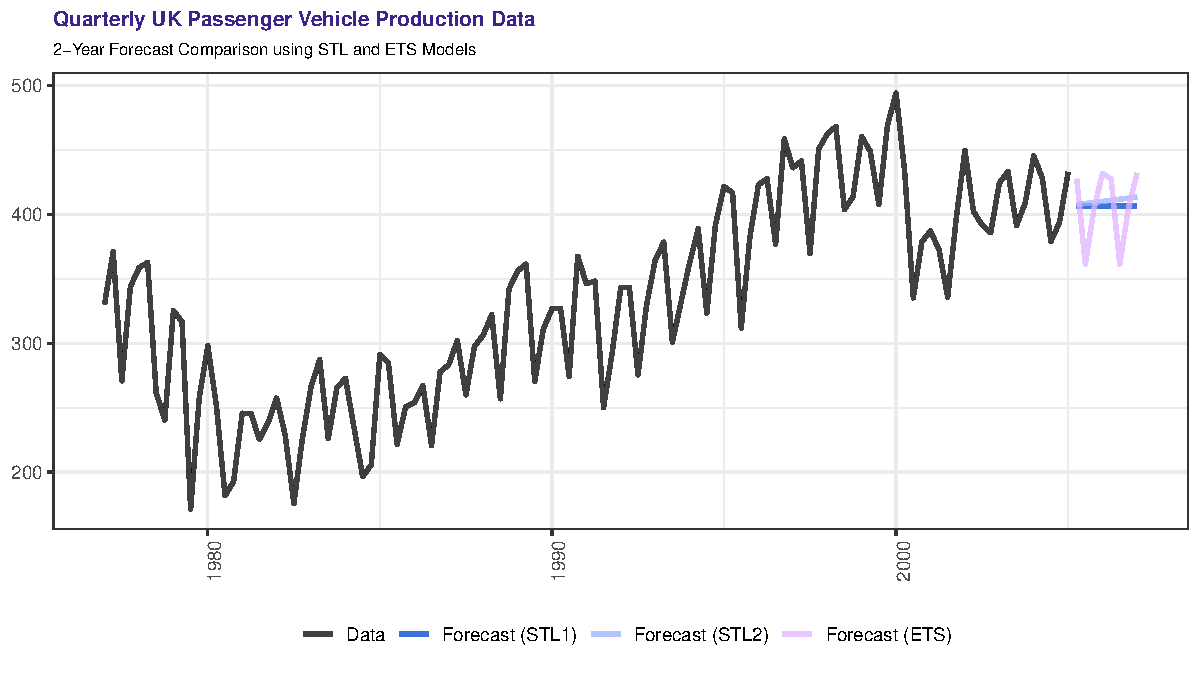
\includegraphics{homework-one_files/figure-latex/ha-7.10g-1.pdf}

\hypertarget{h.-check-the-residuals-of-your-preferred-model.}{%
\subsection{h. Check the residuals of your preferred model.}\label{h.-check-the-residuals-of-your-preferred-model.}}

The plots below contains our residuals data from the preferred ETS model. We observed constant variance and normally distribution of our residuals, suggesting our model has adequately captured the information from the \texttt{ukcars} data

\begin{Shaded}
\begin{Highlighting}[]
\KeywordTok{cbind}\NormalTok{(}\DataTypeTok{Residuals =} \KeywordTok{residuals}\NormalTok{(ukc_ets), }\StringTok{`}\DataTypeTok{Forecast errors}\StringTok{`}\NormalTok{ =}\StringTok{ }\KeywordTok{residuals}\NormalTok{(ukc_ets, }
  \DataTypeTok{type =} \StringTok{"innovation"}\NormalTok{)) }\OperatorTok\StringTok{ }\KeywordTok{autoplot}\NormalTok{(}\DataTypeTok{facet =} \OtherTok{TRUE}\NormalTok{) }\OperatorTok{+}\StringTok{ }\KeywordTok{labs}\NormalTok{(}\DataTypeTok{title =} \StringTok{"Residuals from ETS (A,N,A) model of UKcars data"}\NormalTok{, }
  \DataTypeTok{x =} \StringTok{"Year"}\NormalTok{) }\OperatorTok{+}\StringTok{ }\KeywordTok{theme_bw}\NormalTok{() }\OperatorTok{+}\StringTok{ }\KeywordTok{theme}\NormalTok{()}
\end{Highlighting}
\end{Shaded}

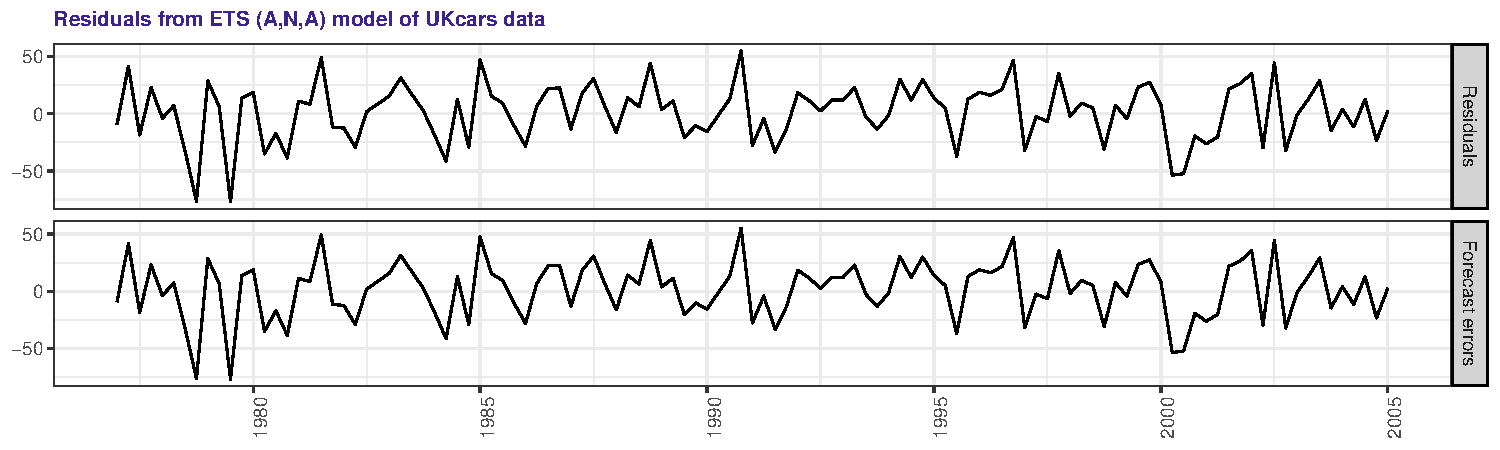
\includegraphics{homework-one_files/figure-latex/ha-7.10h-1.pdf}

\hypertarget{assignment-six}{%
\chapter{Assignment Six}\label{assignment-six}}

\begin{itemize}
\tightlist
\item
  Hyndman 8.1
\item
  Hyndman 8.2
\item
  Hyndman 8.6
\item
  Hyndman 8.8
\end{itemize}

\hypertarget{hyndman-8.1}{%
\section{Hyndman 8.1}\label{hyndman-8.1}}

\hypertarget{a.-explain-the-differences-among-these-figures.-do-they-all-indicate-that-the-data-are-white-noise}{%
\subsection{a. Explain the differences among these figures. Do they all indicate that the data are white noise?}\label{a.-explain-the-differences-among-these-figures.-do-they-all-indicate-that-the-data-are-white-noise}}

ACF plots (also known as correlograms) are used to graph the autocorrelation coeffients of lag values in a timeseries. In white noise series, we expect autocorrelation to be close to zero. This component is observed in the ACF plots by examining the dashed blue lines.

Using this knowledge, we can determine that all three series are white noise because they all show just a small spread between these blue lines and hover around 0. Only two lag lines come close to exceeding this boundary, but none are significant or escape the denoted critical value used to determine autocorrelation.

\hypertarget{b.-why-are-the-critical-values-at-different-distances-from-the-mean-of-zero-why-are-the-autocorrelations-different-in-each-figure-when-they-each-refer-to-white-noise}{%
\subsection{b. Why are the critical values at different distances from the mean of zero? Why are the autocorrelations different in each figure when they each refer to white noise?}\label{b.-why-are-the-critical-values-at-different-distances-from-the-mean-of-zero-why-are-the-autocorrelations-different-in-each-figure-when-they-each-refer-to-white-noise}}

The blue line boundary on an ACF plot is calculated using the formula \(\pm 2 / \sqrt{T-d}\), where \(T\) represents the length of time in a series and \(d\) the number of differences. Thus as \(T\) grows larger, the denominator also gets larger, making the resulting quotient smaller.

This means that the areas defined by the boundaries \(\pm 2 / \sqrt{T-d}\) decrease as the number values in series \(T\) increases.

\hypertarget{hyndman-8.2}{%
\section{Hyndman 8.2}\label{hyndman-8.2}}

A classic example of a non-stationary series is the daily closing IBM stock price series (data set \texttt{ibmclose}). Use R to plot the daily closing prices for IBM stock and the ACF and PACF. Explain how each plot shows that the series is non-stationary and should be differenced.

\hypertarget{a.-time-series-plot}{%
\subsection{a. Time Series Plot}\label{a.-time-series-plot}}

\begin{Shaded}
\begin{Highlighting}[]
\NormalTok{p1 <-}\StringTok{ }\KeywordTok{autoplot}\NormalTok{(ibmclose) }\OperatorTok{+}\StringTok{ }\KeywordTok{labs}\NormalTok{(}\DataTypeTok{title =} \StringTok{"Non-Stationary"}\NormalTok{, }
  \DataTypeTok{y =} \StringTok{"Price"}\NormalTok{, }\DataTypeTok{x =} \StringTok{"Days"}\NormalTok{) }\OperatorTok{+}\StringTok{ }\KeywordTok{theme_bw}\NormalTok{() }\OperatorTok{+}\StringTok{ }\KeywordTok{theme}\NormalTok{()}
\NormalTok{p2 <-}\StringTok{ }\KeywordTok{autoplot}\NormalTok{(}\KeywordTok{diff}\NormalTok{(ibmclose)) }\OperatorTok{+}\StringTok{ }\KeywordTok{labs}\NormalTok{(}\DataTypeTok{title =} \StringTok{"Differenced"}\NormalTok{, }
  \DataTypeTok{y =} \StringTok{"Price"}\NormalTok{, }\DataTypeTok{x =} \StringTok{"Days"}\NormalTok{) }\OperatorTok{+}\StringTok{ }\KeywordTok{theme_bw}\NormalTok{() }\OperatorTok{+}\StringTok{ }\KeywordTok{theme}\NormalTok{()}

\KeywordTok{grid.arrange}\NormalTok{(p1, p2, }\DataTypeTok{ncol =} \DecValTok{2}\NormalTok{, }\DataTypeTok{top =} \StringTok{"Daily Closing IBM Stock Price"}\NormalTok{)}
\end{Highlighting}
\end{Shaded}

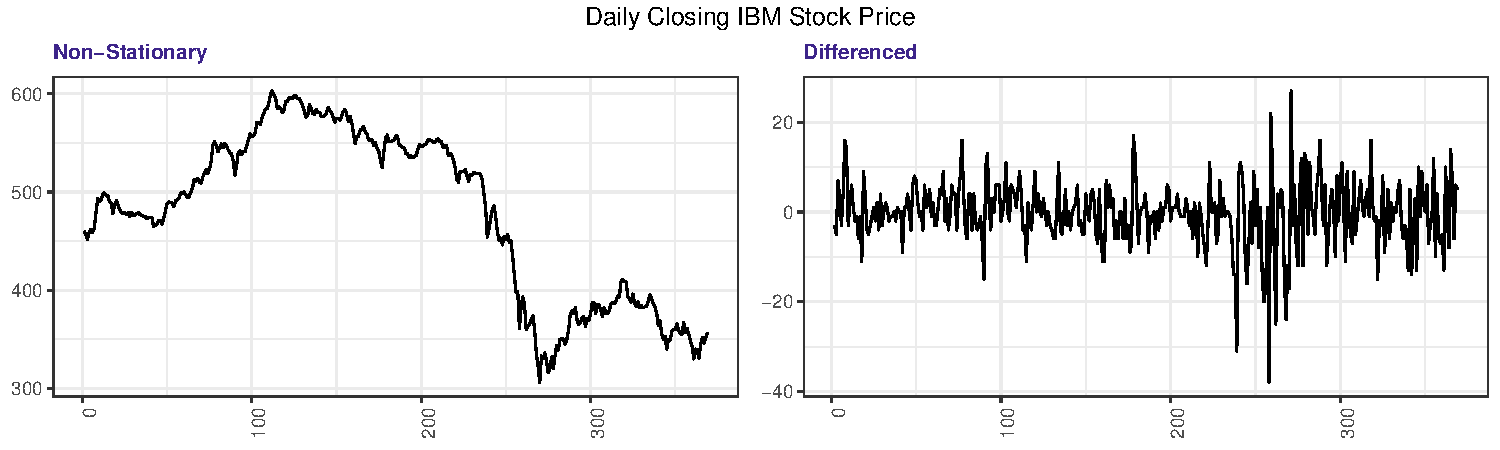
\includegraphics{homework-one_files/figure-latex/8.2a-1.pdf}

Daily closing prices from the \texttt{ibmclose} dataset are non-stationary and show an overall trend component. Seasonality is harder to distinguish at this frequency. There may be a cyclical component where pattern changes occur over a non-specific period of time, however, there are not enough observations to determine this.

We can compare this plot to a differenced timeseries, in which the stock prices are stationary and do not depend on the time at which the series is observed. Stationary models are required for autoregression modeling and analysis.

\hypertarget{b.-acf-plot}{%
\subsection{b. ACF Plot}\label{b.-acf-plot}}

\begin{Shaded}
\begin{Highlighting}[]
\NormalTok{p1 <-}\StringTok{ }\KeywordTok{ggAcf}\NormalTok{(ibmclose) }\OperatorTok{+}\StringTok{ }\KeywordTok{theme_bw}\NormalTok{() }\OperatorTok{+}\StringTok{ }\KeywordTok{theme}\NormalTok{()}
\NormalTok{p2 <-}\StringTok{ }\KeywordTok{ggAcf}\NormalTok{(}\KeywordTok{diff}\NormalTok{(ibmclose)) }\OperatorTok{+}\StringTok{ }\KeywordTok{theme_bw}\NormalTok{() }\OperatorTok{+}\StringTok{ }\KeywordTok{theme}\NormalTok{()}

\KeywordTok{grid.arrange}\NormalTok{(p1, p2, }\DataTypeTok{ncol =} \DecValTok{2}\NormalTok{, }\DataTypeTok{top =} \StringTok{"Daily Closing IBM Stock Price"}\NormalTok{)}
\end{Highlighting}
\end{Shaded}

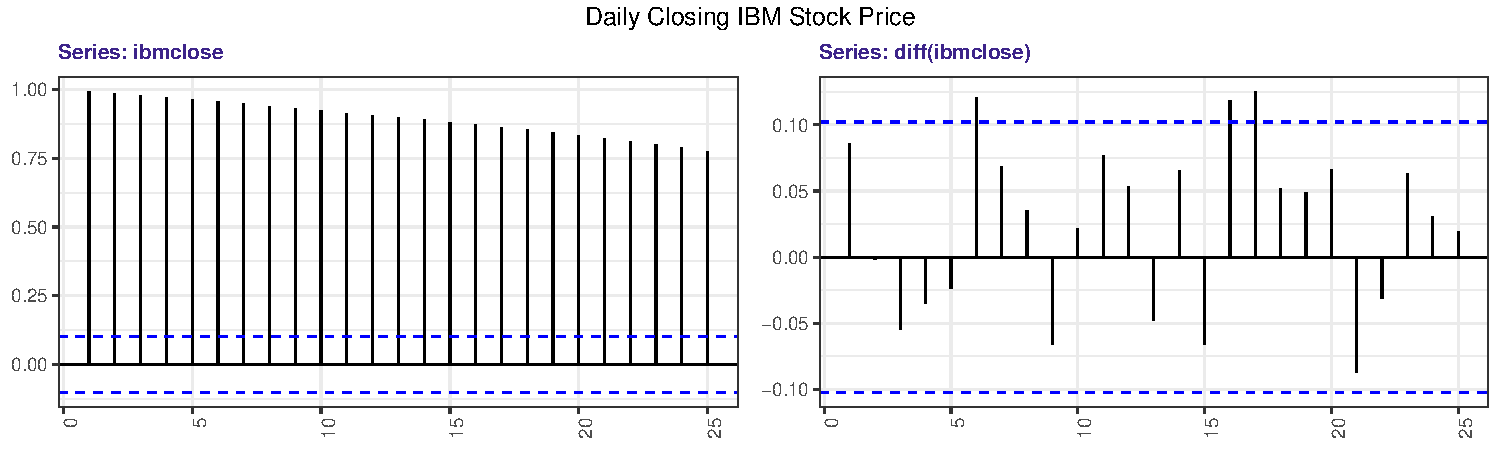
\includegraphics{homework-one_files/figure-latex/8.2b-1.pdf}
In our \texttt{ibmclose} series, we can identify large, positive, and slowly decreasing lags. This further indicates that our data is non-stationary, trended, and autocorrelated. Seasonal fluxuations do not appear present within our lags.

Autoregressive models, however, require stationary data. The \texttt{ibmclose} data could be differenced to meet this requirement. The \texttt{diff(ibmclose)} series has no signs of autocorrelation outside the 95\% limit (\(\pm 0.1\)) as shown by the dashed blue lines. This plot appears similiar to a white noise series.

\hypertarget{c.-pacf-plot}{%
\subsection{c. PACF Plot}\label{c.-pacf-plot}}

\begin{Shaded}
\begin{Highlighting}[]
\NormalTok{p1 <-}\StringTok{ }\KeywordTok{ggPacf}\NormalTok{(ibmclose) }\OperatorTok{+}\StringTok{ }\KeywordTok{ggtitle}\NormalTok{(}\StringTok{"`ibmclose Series ACF"}\NormalTok{) }\OperatorTok{+}\StringTok{ }
\StringTok{  }\KeywordTok{theme_bw}\NormalTok{() }\OperatorTok{+}\StringTok{ }\KeywordTok{theme}\NormalTok{()}
\NormalTok{p2 <-}\StringTok{ }\KeywordTok{ggPacf}\NormalTok{(}\KeywordTok{diff}\NormalTok{(ibmclose)) }\OperatorTok{+}\StringTok{ }\KeywordTok{ggtitle}\NormalTok{(}\StringTok{"`ibmclose` ACF Differenced Series"}\NormalTok{) }\OperatorTok{+}\StringTok{ }
\StringTok{  }\KeywordTok{theme_bw}\NormalTok{() }\OperatorTok{+}\StringTok{ }\KeywordTok{theme}\NormalTok{()}

\KeywordTok{grid.arrange}\NormalTok{(p1, p2, }\DataTypeTok{ncol =} \DecValTok{2}\NormalTok{, }\DataTypeTok{top =} \StringTok{"Daily Closing IBM Stock Price"}\NormalTok{)}
\end{Highlighting}
\end{Shaded}

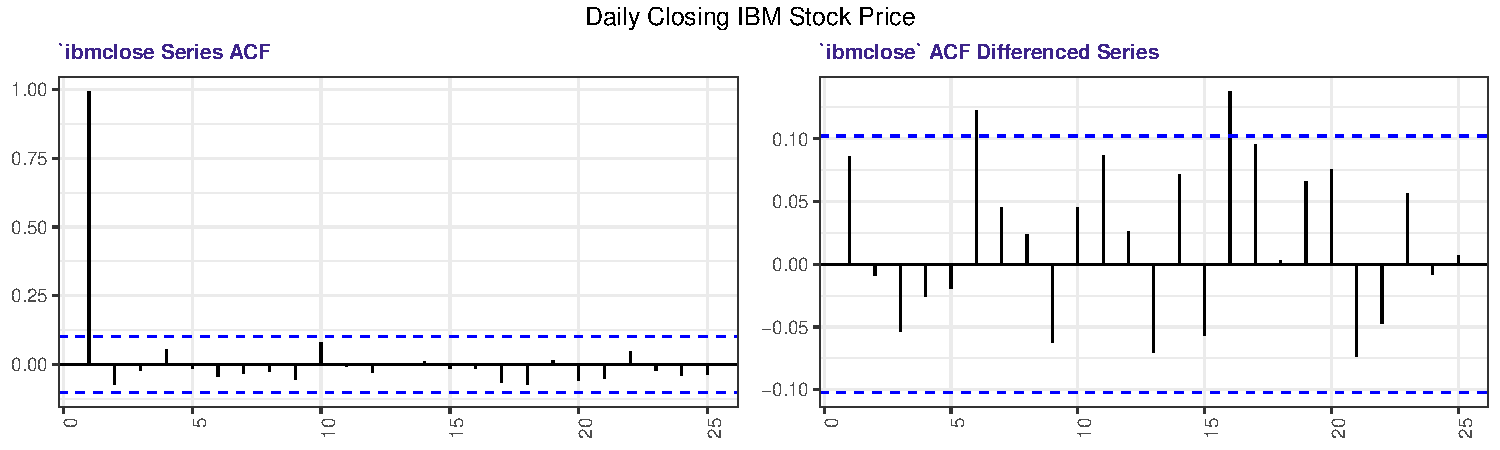
\includegraphics{homework-one_files/figure-latex/8.2c-1.pdf}

Lastly, the PACF plot is used to look at partial autocorrelation. This plot analyzes the correlation of residuals after removing the effect explained by previous lags. Our Pacf plot of the \texttt{ibmclose} series a sharp cut off after the first lag.

Pacf is very beneficial in determining order of moving averages component of a non-seasonal ARIMA model. In the differentiated data, there are two spikes outside the 95\% limit. These can be ignored though as they do not occur in our initial lags and fall just outside the \(\pm 0.1\) limit. The differentiated Pacf plot further suggests a white-noise ARIMA model of the stationary data.

\hypertarget{hyndman-8.6}{%
\section{Hyndman 8.6}\label{hyndman-8.6}}

Use R to simulate and plot some data from simple ARIMA models.

\hypertarget{a.-use-the-following-r-code-to-generate-data-from-an-ar1-model-with-phi_10.6-and-sigma21.-the-process-starts-with-y_10.}{%
\subsection{\texorpdfstring{a. Use the following R code to generate data from an AR(1) model with \(\phi_1=0.6\) and \(\sigma^2=1\). The process starts with \(y_1=0\).}{a. Use the following R code to generate data from an AR(1) model with \textbackslash{}phi\_1=0.6 and \textbackslash{}sigma\^{}2=1. The process starts with y\_1=0.}}\label{a.-use-the-following-r-code-to-generate-data-from-an-ar1-model-with-phi_10.6-and-sigma21.-the-process-starts-with-y_10.}}

\begin{Shaded}
\begin{Highlighting}[]
\CommentTok{# Sample Code}
\NormalTok{y <-}\StringTok{ }\KeywordTok{ts}\NormalTok{(}\KeywordTok{numeric}\NormalTok{(}\DecValTok{100}\NormalTok{))}
\NormalTok{e <-}\StringTok{ }\KeywordTok{rnorm}\NormalTok{(}\DecValTok{100}\NormalTok{)}
\ControlFlowTok{for}\NormalTok{ (i }\ControlFlowTok{in} \DecValTok{2}\OperatorTok{:}\DecValTok{100}\NormalTok{) y[i] <-}\StringTok{ }\FloatTok{0.6} \OperatorTok{*}\StringTok{ }\NormalTok{y[i }\OperatorTok{-}\StringTok{ }\DecValTok{1}\NormalTok{] }\OperatorTok{+}\StringTok{ }\NormalTok{e[i]}

\CommentTok{# Function}

\NormalTok{AR1 <-}\StringTok{ }\ControlFlowTok{function}\NormalTok{(phi1, sigma2, c) \{}
  \CommentTok{# add warnings for expected constraints for AR1}
  \CommentTok{# parameters values}
  \ControlFlowTok{if}\NormalTok{ (phi1 }\OperatorTok{<}\StringTok{ }\DecValTok{-1}\NormalTok{) }
    \KeywordTok{warning}\NormalTok{(}\StringTok{"'phi1' should be > -1 for AR(1) models"}\NormalTok{)}
  \ControlFlowTok{if}\NormalTok{ (phi1 }\OperatorTok{>}\StringTok{ }\DecValTok{1}\NormalTok{) }
    \KeywordTok{warning}\NormalTok{(}\StringTok{"'phi1' should be < 1 for AR(1) models"}\NormalTok{)}
  \ControlFlowTok{if}\NormalTok{ (phi1 }\OperatorTok{<}\StringTok{ }\DecValTok{1} \OperatorTok{&}\StringTok{ }\NormalTok{phi1 }\OperatorTok{>}\StringTok{ }\DecValTok{-1}\NormalTok{) }
    \KeywordTok{message}\NormalTok{(}\StringTok{"Model: AR(1) "}\NormalTok{)}
  
  \CommentTok{# set random number generation (RNG) state}
  \KeywordTok{set.seed}\NormalTok{(}\DecValTok{5}\NormalTok{)}
  
  \CommentTok{# generate time series 1:100}
\NormalTok{  y <-}\StringTok{ }\KeywordTok{ts}\NormalTok{(}\KeywordTok{numeric}\NormalTok{(}\DecValTok{100}\NormalTok{))}
  
  \CommentTok{# RNG of epsilon with constant variance (sigma^2)}
\NormalTok{  e <-}\StringTok{ }\KeywordTok{rnorm}\NormalTok{(}\DecValTok{100}\NormalTok{, }\DataTypeTok{sd =}\NormalTok{ sigma2)}
  
  \CommentTok{# apply formula to all but the first ts observation so}
  \CommentTok{# that y1=0}
  \ControlFlowTok{for}\NormalTok{ (i }\ControlFlowTok{in} \DecValTok{2}\OperatorTok{:}\DecValTok{100}\NormalTok{) \{}
\NormalTok{    y[i] <-}\StringTok{ }\NormalTok{c }\OperatorTok{+}\StringTok{ }\NormalTok{phi1 }\OperatorTok{*}\StringTok{ }\NormalTok{y[i }\OperatorTok{-}\StringTok{ }\DecValTok{1}\NormalTok{] }\OperatorTok{+}\StringTok{ }\NormalTok{e[i]}
\NormalTok{  \}}
  \KeywordTok{return}\NormalTok{(y)}
\NormalTok{\}}

\CommentTok{# Set parameters per instruction}
\NormalTok{phi1 =}\StringTok{ }\FloatTok{0.6}
\NormalTok{sigma2 =}\StringTok{ }\DecValTok{1}
\NormalTok{c =}\StringTok{ }\DecValTok{0}

\CommentTok{# Generate Data}
\KeywordTok{AR1}\NormalTok{(phi1, sigma2, c)}
\end{Highlighting}
\end{Shaded}

\begin{verbatim}
FALSE Time Series:
FALSE Start = 1 
FALSE End = 100 
FALSE Frequency = 1 
FALSE   [1]  0.00000000  1.38435934 -0.42487626 -0.18478299
FALSE   [5]  1.60057108  0.35743467 -0.25770559 -0.78999466
FALSE   [9] -0.75977043 -0.31775404  1.03697792 -0.17959270
FALSE  [13] -1.18814822 -0.87042329 -1.59401401 -1.09539455
FALSE  [17] -1.25454982 -2.93669665 -1.52120074 -1.17207585
FALSE  [21]  0.19726644  1.06022926  2.10409946  1.96922076
FALSE  [25]  2.00054139  0.90684298  1.96269486  2.67639075
FALSE  [29]  0.94875235 -0.28354403  0.14578862  1.19716734
FALSE  [33]  2.93376098  2.97736022  3.26563792  2.91095659
FALSE  [37]  0.73704131 -1.55824796 -2.69713465 -1.76088891
FALSE  [41]  0.49352702 -0.50630697 -0.37836310  1.66865009
FALSE  [45]  0.54462112  0.88899603 -0.35361089 -0.67241111
FALSE  [49] -1.12777515 -0.74587625  1.01572281  0.79715979
FALSE  [53]  1.50031873  0.30835641  0.07281319 -0.88126517
FALSE  [57]  0.22454569  0.02211835 -0.05081992  0.20278334
FALSE  [61] -1.01491280  0.24588274 -0.43084077  0.23785708
FALSE  [65] -0.61734369 -0.71179248 -2.52940461 -1.81934505
FALSE  [69] -2.36399047 -1.69806039 -1.22293356 -0.95937432
FALSE  [73] -0.22859614 -0.10478984  0.35065739  0.05504595
FALSE  [77]  1.00651297  0.72499792  0.62417244 -0.18838160
FALSE  [81]  0.38538720 -1.51107017  0.06888699  0.01724932
FALSE  [85]  0.68603407 -0.29868916  2.20801915  0.85137948
FALSE  [89]  0.43505513 -0.26080698  0.76956295 -0.60067340
FALSE  [93]  0.19662982  1.01870848  1.60117077  1.34431055
FALSE  [97]  0.46000252 -0.26418774 -0.34106824 -0.26394059
\end{verbatim}

\hypertarget{b.-produce-a-time-plot-for-the-series.-how-does-the-plot-change-as-you-change-phi_1}{%
\subsection{\texorpdfstring{b. Produce a time plot for the series. How does the plot change as you change \(\phi_1\)?}{b. Produce a time plot for the series. How does the plot change as you change \textbackslash{}phi\_1?}}\label{b.-produce-a-time-plot-for-the-series.-how-does-the-plot-change-as-you-change-phi_1}}

\begin{Shaded}
\begin{Highlighting}[]
\NormalTok{nam <-}\StringTok{ }\KeywordTok{expression}\NormalTok{(phi[}\DecValTok{1}\NormalTok{])}

\NormalTok{AR1_phi1 <-}\StringTok{ }\KeywordTok{suppressMessages}\NormalTok{(}\KeywordTok{cbind}\NormalTok{(}\StringTok{`}\DataTypeTok{-0.9}\StringTok{`}\NormalTok{ =}\StringTok{ }\KeywordTok{AR1}\NormalTok{(}\OperatorTok{-}\FloatTok{0.9}\NormalTok{, }\DecValTok{1}\NormalTok{, }
  \DecValTok{0}\NormalTok{), }\StringTok{`}\DataTypeTok{-0.6}\StringTok{`}\NormalTok{ =}\StringTok{ }\KeywordTok{AR1}\NormalTok{(}\OperatorTok{-}\FloatTok{0.6}\NormalTok{, }\DecValTok{1}\NormalTok{, }\DecValTok{0}\NormalTok{), }\StringTok{`}\DataTypeTok{0.0}\StringTok{`}\NormalTok{ =}\StringTok{ }\KeywordTok{AR1}\NormalTok{(}\DecValTok{0}\NormalTok{, }\DecValTok{1}\NormalTok{, }\DecValTok{0}\NormalTok{), }\StringTok{`}\DataTypeTok{0.6}\StringTok{`}\NormalTok{ =}\StringTok{ }\KeywordTok{AR1}\NormalTok{(}\FloatTok{0.6}\NormalTok{, }
  \DecValTok{1}\NormalTok{, }\DecValTok{0}\NormalTok{), }\StringTok{`}\DataTypeTok{0.9}\StringTok{`}\NormalTok{ =}\StringTok{ }\KeywordTok{AR1}\NormalTok{(}\FloatTok{0.9}\NormalTok{, }\DecValTok{1}\NormalTok{, }\DecValTok{0}\NormalTok{)))}

\NormalTok{pallete =}\StringTok{ }\KeywordTok{c}\NormalTok{(}\StringTok{"#dfb1c5"}\NormalTok{, }\StringTok{"#86d1f1"}\NormalTok{, }\StringTok{"#000000"}\NormalTok{, }\StringTok{"#5ead7f"}\NormalTok{, }\StringTok{"#a931a1"}\NormalTok{)}
\CommentTok{# palette <- brewer.pal(n = 5 , name = 'RdYlGn')}
\NormalTok{palette <-}\StringTok{ }\KeywordTok{c}\NormalTok{(}\StringTok{"#D7191C"}\NormalTok{, }\StringTok{"#C51B8A"}\NormalTok{, }\StringTok{"#555555"}\NormalTok{, }\StringTok{"#756BB1"}\NormalTok{, }
  \StringTok{"#2C7BB6"}\NormalTok{)}
\KeywordTok{autoplot}\NormalTok{(AR1_phi1, }\DataTypeTok{size =} \FloatTok{0.25}\NormalTok{, }\DataTypeTok{alpha =} \FloatTok{0.9}\NormalTok{) }\OperatorTok{+}\StringTok{ }\KeywordTok{scale_color_manual}\NormalTok{(}\DataTypeTok{name =}\NormalTok{ nam, }
  \DataTypeTok{values =}\NormalTok{ pallete) }\OperatorTok{+}\StringTok{ }\KeywordTok{labs}\NormalTok{(}\DataTypeTok{title =} \StringTok{"Time Plot of AR(1) Model Series"}\NormalTok{, }
  \DataTypeTok{subtitle =} \KeywordTok{expression}\NormalTok{(}\StringTok{"Display of Changes in"} \OperatorTok{~}\StringTok{ }\NormalTok{phi }\OperatorTok{~}\StringTok{ }
\StringTok{    "when c=0"}\NormalTok{), }\DataTypeTok{y =} \StringTok{"Value"}\NormalTok{) }\OperatorTok{+}\StringTok{ }\KeywordTok{theme_bw}\NormalTok{() }\OperatorTok{+}\StringTok{ }\KeywordTok{theme}\NormalTok{(}\DataTypeTok{legend.position =} \StringTok{"bottom"}\NormalTok{)}
\end{Highlighting}
\end{Shaded}

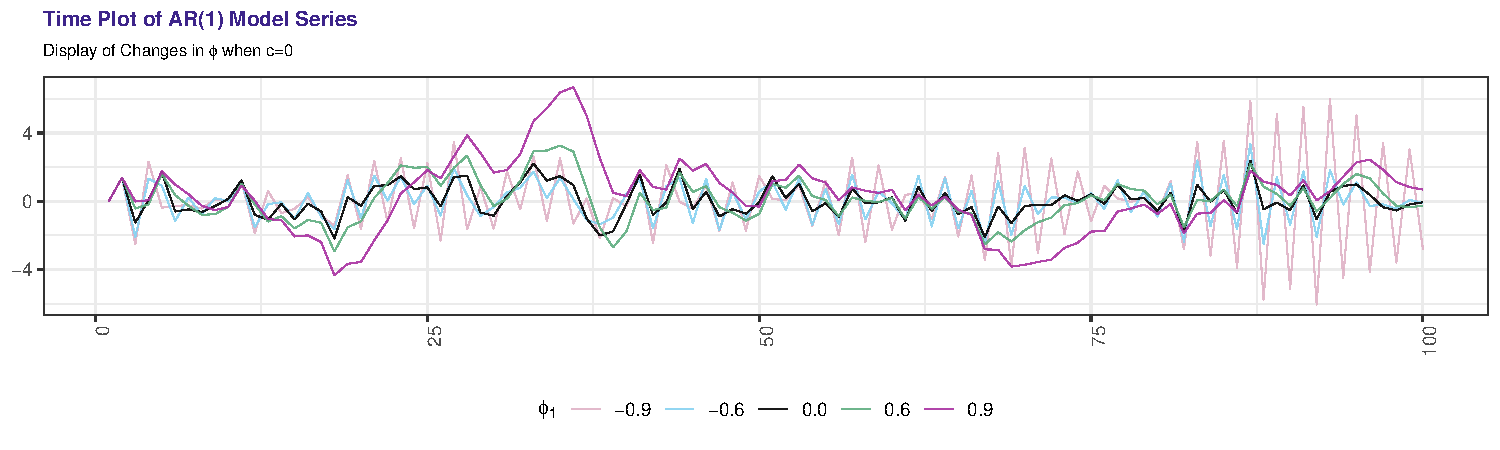
\includegraphics{homework-one_files/figure-latex/8.6b-1.pdf}

\begin{itemize}
\tightlist
\item
  The AR(1) Model at \(\phi=0\) should be the equivalent of white noise.\\
\item
  The \(y_t\) is expected to oscillate around the mean when \(\phi<0\).\\
\item
  We would expect \(y_t\) to resemble a random walk when \(\phi=1\) and \(c=0\).
\end{itemize}

As expected we observe these patterns in the time series plots above. The variation and pattern observed in \(y\) changes as the \(\phi\) parameter changes with the negative values of \(\phi\) occilating around the mean, and the positive numbers becoming more like a random walk as \(\phi\) approaches 1.

\hypertarget{c.-write-your-own-code-to-generate-data-from-an-ma1-model-with-theta_10.6-and-sigma21.}{%
\subsection{\texorpdfstring{c. Write your own code to generate data from an MA(1) model with \(\theta_1=0.6\) and \(sigma^2=1\).}{c. Write your own code to generate data from an MA(1) model with \textbackslash{}theta\_1=0.6 and sigma\^{}2=1.}}\label{c.-write-your-own-code-to-generate-data-from-an-ma1-model-with-theta_10.6-and-sigma21.}}

\begin{Shaded}
\begin{Highlighting}[]
\CommentTok{# Function}
\NormalTok{MA1 <-}\StringTok{ }\ControlFlowTok{function}\NormalTok{(theta1, sigma2, c) \{}
  \CommentTok{# add warnings for expected constraints for MA1}
  \CommentTok{# parameters values}
  \ControlFlowTok{if}\NormalTok{ (theta1 }\OperatorTok{<}\StringTok{ }\DecValTok{0}\NormalTok{) }
    \KeywordTok{warning}\NormalTok{(}\StringTok{"'theta' should be > 0 for MA(1) models"}\NormalTok{)}
  \ControlFlowTok{if}\NormalTok{ (theta1 }\OperatorTok{>}\StringTok{ }\DecValTok{1}\NormalTok{) }
    \KeywordTok{warning}\NormalTok{(}\StringTok{"'theta' should be < 1 for MA(1) models"}\NormalTok{)}
  \ControlFlowTok{if}\NormalTok{ (theta1 }\OperatorTok{<}\StringTok{ }\DecValTok{1} \OperatorTok{&}\StringTok{ }\NormalTok{theta1 }\OperatorTok{>}\StringTok{ }\DecValTok{0}\NormalTok{) }
    \KeywordTok{message}\NormalTok{(}\StringTok{"Model: MA(1)"}\NormalTok{)}
  
  \CommentTok{# set random number generation (RNG) state}
  \KeywordTok{set.seed}\NormalTok{(}\DecValTok{5}\NormalTok{)}
  
  \CommentTok{# generate time series 1:100}
\NormalTok{  y <-}\StringTok{ }\KeywordTok{ts}\NormalTok{(}\KeywordTok{numeric}\NormalTok{(}\DecValTok{100}\NormalTok{))}
  
  \CommentTok{# RNG of epsilon with constant variance (sigma^2)}
\NormalTok{  e <-}\StringTok{ }\KeywordTok{rnorm}\NormalTok{(}\DecValTok{100}\NormalTok{, }\DataTypeTok{sd =}\NormalTok{ sigma2)}
  
  \CommentTok{# apply formula to all but the first ts observation so}
  \CommentTok{# that y1=0}
  \ControlFlowTok{for}\NormalTok{ (i }\ControlFlowTok{in} \DecValTok{2}\OperatorTok{:}\DecValTok{100}\NormalTok{) \{}
\NormalTok{    y[i] <-}\StringTok{ }\NormalTok{c }\OperatorTok{+}\StringTok{ }\NormalTok{theta1 }\OperatorTok{*}\StringTok{ }\NormalTok{e[i }\OperatorTok{-}\StringTok{ }\DecValTok{1}\NormalTok{] }\OperatorTok{+}\StringTok{ }\NormalTok{e[i]}
\NormalTok{  \}}
  \KeywordTok{return}\NormalTok{(y)}
\NormalTok{\}}

\CommentTok{# Set parameters per instruction}
\NormalTok{theta1 =}\StringTok{ }\FloatTok{0.6}
\NormalTok{sigma2 =}\StringTok{ }\DecValTok{1}
\NormalTok{c =}\StringTok{ }\DecValTok{0}

\CommentTok{# Generate Data}
\KeywordTok{MA1}\NormalTok{(theta1, sigma2, c)}
\end{Highlighting}
\end{Shaded}

\begin{verbatim}
FALSE Time Series:
FALSE Start = 1 
FALSE End = 100 
FALSE Frequency = 1 
FALSE   [1]  0.00000000  0.87984606 -0.42487626 -0.68315235
FALSE   [5]  1.75352653  0.42395654 -0.83391117 -0.91867114
FALSE   [9] -0.66699642 -0.03335596  1.31049528 -0.06520125
FALSE  [13] -1.56146027 -0.80576992 -1.16628065 -0.78204216
FALSE  [17] -0.68070478 -2.54235462 -1.06956280 -0.11486505
FALSE  [21]  0.74489870  1.48217656  2.03308354  1.58753823
FALSE  [25]  1.24306558  0.19792351  1.24249996  2.34992727
FALSE  [29]  0.24218220 -1.24704470 -0.19576223  1.29924319
FALSE  [33]  2.88127707  2.54637998  2.20948397  1.83910690
FALSE  [37] -0.43858835 -2.60619233 -2.96246952 -1.19991965
FALSE  [41]  1.46449549  0.12761304 -0.55603283  1.85092060
FALSE  [45]  0.68083183  0.28828200 -0.54967449 -0.99244968
FALSE  [49] -1.00047523 -0.50380825  1.42172187  1.06567524
FALSE  [53]  1.13465852  0.02137888 -0.46730155 -0.99227348
FALSE  [57]  0.19833295  0.33937381 -0.13165637  0.19482074
FALSE  [61] -0.99661763  0.17288074 -0.06547217  0.14933929
FALSE  [65] -0.46224101 -0.79742103 -2.30716088 -1.56309975
FALSE  [69] -1.45340481 -1.04309618 -0.37189699 -0.34807258
FALSE  [73]  0.21165994  0.24058491  0.43295200  0.09277030
FALSE  [77]  0.88027631  0.70518138  0.26182778 -0.44938085
FALSE  [81]  0.16068512 -1.44325279 -0.06985240  0.56123459
FALSE  [85]  0.66123475 -0.30489892  1.96104688  0.95890758
FALSE  [89] -0.35983176 -0.56730359  0.61294310 -0.50678289
FALSE  [93] -0.08041284  1.23495090  1.53038403  0.97757550
FALSE  [97] -0.11641896 -0.74813954 -0.50666914 -0.16883301
\end{verbatim}

\hypertarget{d.-produce-a-time-plot-for-the-series.-how-does-the-plot-change-as-you-change-theta_1}{%
\subsection{\texorpdfstring{d. Produce a time plot for the series. How does the plot change as you change \(\theta_1\)?}{d. Produce a time plot for the series. How does the plot change as you change \textbackslash{}theta\_1?}}\label{d.-produce-a-time-plot-for-the-series.-how-does-the-plot-change-as-you-change-theta_1}}

\begin{Shaded}
\begin{Highlighting}[]
\NormalTok{nam <-}\StringTok{ }\KeywordTok{expression}\NormalTok{(theta[}\DecValTok{1}\NormalTok{])}

\NormalTok{MA1_theta1 <-}\StringTok{ }\KeywordTok{cbind}\NormalTok{(}\StringTok{`}\DataTypeTok{0.1}\StringTok{`}\NormalTok{ =}\StringTok{ }\KeywordTok{suppressMessages}\NormalTok{(}\KeywordTok{MA1}\NormalTok{(}\FloatTok{0.1}\NormalTok{, }\DecValTok{1}\NormalTok{, }
  \DecValTok{0}\NormalTok{)), }\StringTok{`}\DataTypeTok{0.3}\StringTok{`}\NormalTok{ =}\StringTok{ }\KeywordTok{suppressMessages}\NormalTok{(}\KeywordTok{MA1}\NormalTok{(}\FloatTok{0.3}\NormalTok{, }\DecValTok{1}\NormalTok{, }\DecValTok{0}\NormalTok{)), }\StringTok{`}\DataTypeTok{0.6}\StringTok{`}\NormalTok{ =}\StringTok{ }\KeywordTok{suppressMessages}\NormalTok{(}\KeywordTok{MA1}\NormalTok{(}\FloatTok{0.6}\NormalTok{, }
  \DecValTok{1}\NormalTok{, }\DecValTok{0}\NormalTok{)), }\StringTok{`}\DataTypeTok{0.9}\StringTok{`}\NormalTok{ =}\StringTok{ }\KeywordTok{suppressMessages}\NormalTok{(}\KeywordTok{MA1}\NormalTok{(}\FloatTok{0.9}\NormalTok{, }\DecValTok{1}\NormalTok{, }\DecValTok{0}\NormalTok{)))}

\NormalTok{pallete =}\StringTok{ }\KeywordTok{c}\NormalTok{(}\StringTok{"#d74887"}\NormalTok{, }\StringTok{"#000000"}\NormalTok{, }\StringTok{"#86d1f1"}\NormalTok{, }\StringTok{"#5ead7f"}\NormalTok{)}

\KeywordTok{autoplot}\NormalTok{(}\KeywordTok{suppressMessages}\NormalTok{(MA1_theta1), }\DataTypeTok{size =} \FloatTok{0.5}\NormalTok{, }\DataTypeTok{alpha =} \FloatTok{0.8}\NormalTok{) }\OperatorTok{+}\StringTok{ }
\StringTok{  }\KeywordTok{scale_color_manual}\NormalTok{(}\DataTypeTok{name =}\NormalTok{ nam, }\DataTypeTok{values =}\NormalTok{ pallete) }\OperatorTok{+}\StringTok{ }\KeywordTok{labs}\NormalTok{(}\DataTypeTok{title =} \StringTok{"Time Plot of MA(1) Model Series"}\NormalTok{, }
  \DataTypeTok{subtitle =} \KeywordTok{expression}\NormalTok{(}\StringTok{"Display of Changes in"} \OperatorTok{~}\StringTok{ }\NormalTok{theta[}\DecValTok{1}\NormalTok{] }\OperatorTok{~}\StringTok{ }
\StringTok{    "when c=0 and"} \OperatorTok{~}\StringTok{ }\NormalTok{sigma}\OperatorTok{^}\DecValTok{2} \OperatorTok{~}\StringTok{ "=1"}\NormalTok{), }\DataTypeTok{y =} \StringTok{"Value"}\NormalTok{) }\OperatorTok{+}\StringTok{ }
\StringTok{  }\KeywordTok{theme_bw}\NormalTok{() }\OperatorTok{+}\StringTok{ }\KeywordTok{theme}\NormalTok{(}\DataTypeTok{legend.position =} \StringTok{"bottom"}\NormalTok{)}
\end{Highlighting}
\end{Shaded}

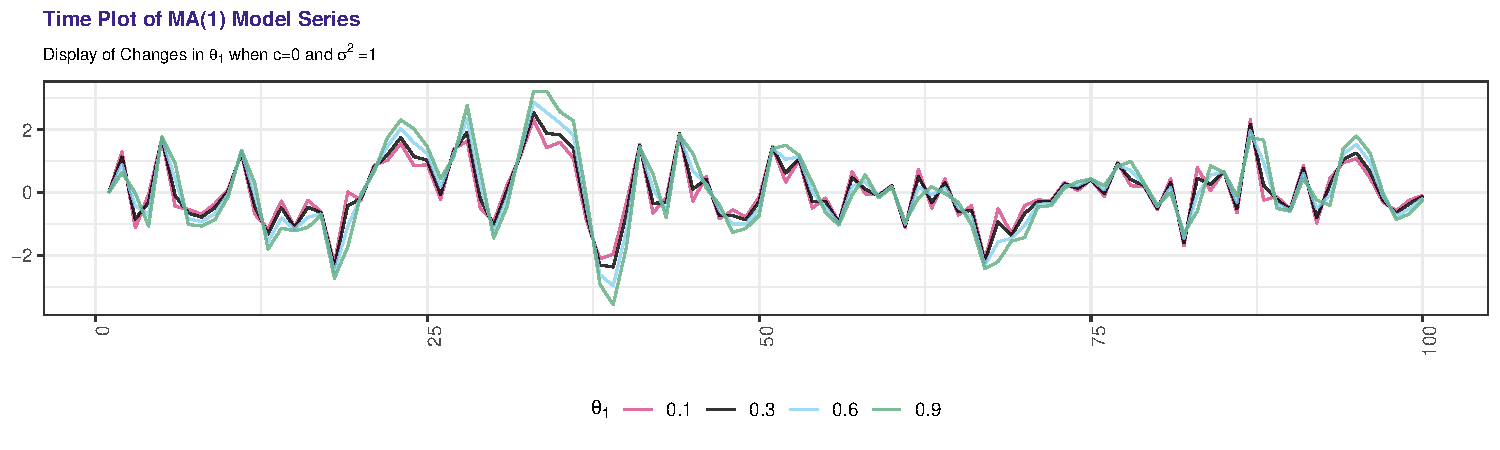
\includegraphics{homework-one_files/figure-latex/8.6d-1.pdf}

\begin{itemize}
\item
  When \(\theta_1\) increases, we observe higher peaks and troughs in the \(y_t\) value.
\item
  In a MA(1) model, we expect the weight of the moving average to be the most constant when \(\theta_1\) nears the value of 1.
\item
  Conversely, the most recent observations have more influence on \(y_t\) than past observations when \(\theta_1<1\).
\end{itemize}

\hypertarget{e.-generate-data-from-an-arma11-model-with-phi_10.6-theta_10.6-and-sigma21.}{%
\subsection{\texorpdfstring{e. Generate data from an ARMA(1,1) model with \(\phi_1=0.6\), \(\theta_1=0.6\), and \(\sigma^2=1\).}{e. Generate data from an ARMA(1,1) model with \textbackslash{}phi\_1=0.6, \textbackslash{}theta\_1=0.6, and \textbackslash{}sigma\^{}2=1.}}\label{e.-generate-data-from-an-arma11-model-with-phi_10.6-theta_10.6-and-sigma21.}}

\begin{Shaded}
\begin{Highlighting}[]
\CommentTok{# Reference ARMA(1,1) Equation:}
\CommentTok{# http://feldman.faculty.pstat.ucsb.edu/174-03/lectures/l7.pdf}

\CommentTok{# Function}
\NormalTok{ARMA11 <-}\StringTok{ }\ControlFlowTok{function}\NormalTok{(phi1, theta1, sigma2, c) \{}
  \CommentTok{# add warnings for expected constraints for ARMA(1,1)}
  \CommentTok{# parameters values}
  \ControlFlowTok{if}\NormalTok{ (phi1 }\OperatorTok{+}\StringTok{ }\NormalTok{theta1 }\OperatorTok{==}\StringTok{ }\DecValTok{0}\NormalTok{) }
    \KeywordTok{warning}\NormalTok{(}\StringTok{"'phi1 + theta1' should be != 0 for ARMA(1,1) models "}\NormalTok{)}
  \ControlFlowTok{if}\NormalTok{ (phi1 }\OperatorTok{+}\StringTok{ }\NormalTok{theta1 }\OperatorTok{!=}\StringTok{ }\DecValTok{0}\NormalTok{) }
    \KeywordTok{message}\NormalTok{(}\StringTok{"Model: ARMA(1,1) "}\NormalTok{)}
  \CommentTok{# set random number generation (RNG) state}
  \KeywordTok{set.seed}\NormalTok{(}\DecValTok{5}\NormalTok{)}
  \CommentTok{# generate time series 1:100}
\NormalTok{  y <-}\StringTok{ }\KeywordTok{ts}\NormalTok{(}\KeywordTok{numeric}\NormalTok{(}\DecValTok{100}\NormalTok{))}
  \CommentTok{# RNG of epsilon with constant variance (sigma^2)}
\NormalTok{  e <-}\StringTok{ }\KeywordTok{rnorm}\NormalTok{(}\DecValTok{100}\NormalTok{, }\DataTypeTok{sd =}\NormalTok{ sigma2)}
  \CommentTok{# apply formula to all but the first ts observation so}
  \CommentTok{# that y1=0}
  \ControlFlowTok{for}\NormalTok{ (t }\ControlFlowTok{in} \DecValTok{2}\OperatorTok{:}\DecValTok{100}\NormalTok{) \{}
\NormalTok{    y[t] <-}\StringTok{ }\NormalTok{phi1 }\OperatorTok{*}\StringTok{ }\NormalTok{y[t }\OperatorTok{-}\StringTok{ }\DecValTok{1}\NormalTok{] }\OperatorTok{+}\StringTok{ }\NormalTok{e[t] }\OperatorTok{+}\StringTok{ }\NormalTok{theta1 }\OperatorTok{*}\StringTok{ }\NormalTok{e[t }\OperatorTok{-}\StringTok{ }\DecValTok{1}\NormalTok{]}
\NormalTok{  \}}
  \KeywordTok{return}\NormalTok{(y)}
\NormalTok{\}}

\CommentTok{# Set parameters per instruction}
\NormalTok{phi1 =}\StringTok{ }\FloatTok{0.6}
\NormalTok{theta1 =}\StringTok{ }\FloatTok{0.6}
\NormalTok{sigma2 =}\StringTok{ }\DecValTok{1}
\NormalTok{c =}\StringTok{ }\DecValTok{0}

\CommentTok{# Generate Data}
\NormalTok{e <-}\StringTok{ }\KeywordTok{ARMA11}\NormalTok{(phi1, theta1, sigma2, c)}
\NormalTok{e}
\end{Highlighting}
\end{Shaded}

\begin{verbatim}
FALSE Time Series:
FALSE Start = 1 
FALSE End = 100 
FALSE Frequency = 1 
FALSE   [1]  0.0000000000  0.8798460550  0.1030313765
FALSE   [4] -0.6213335253  1.3807264174  1.2523923926
FALSE   [7] -0.0824757385 -0.9681565867 -1.2478903744
FALSE  [10] -0.7820901808  0.8412411703  0.4395434538
FALSE  [13] -1.2977342005 -1.5844104364 -2.1169269154
FALSE  [16] -2.0521983137 -1.9120237673 -3.6895688773
FALSE  [19] -3.2833041265 -2.0848475291 -0.5060098161
FALSE  [22]  1.1785706714  2.7402259426  3.2316737972
FALSE  [25]  3.1820698623  2.1071654268  2.5067992194
FALSE  [28]  3.8540068025  2.5545862835  0.2857070734
FALSE  [31] -0.0243379816  1.2846404017  3.6520613133
FALSE  [34]  4.7376167699  5.0520540320  4.8703393236
FALSE  [37]  2.4836152476 -1.1160231776 -3.6320834222
FALSE  [40] -3.3791697028 -0.5630063277 -0.2101907567
FALSE  [43] -0.6821472829  1.4416322330  1.5458111717
FALSE  [46]  1.2157687011  0.1797867268 -0.8845776470
FALSE  [49] -1.5312218200 -1.4225413395  0.5681970658
FALSE  [52]  1.4065934747  1.9786146046  1.2085476466
FALSE  [55]  0.2578270332 -0.8375772590 -0.3042134086
FALSE  [58]  0.1568457636 -0.0375489122  0.1722913893
FALSE  [61] -0.8932427934 -0.3630649348 -0.2833111260
FALSE  [64] -0.0206473879 -0.4746294400 -1.0821986927
FALSE  [67] -2.9564800984 -3.3369878127 -3.4555974986
FALSE  [70] -3.1164546743 -2.2417697913 -1.6931344528
FALSE  [73] -0.8042207310 -0.2419475248  0.2877834804
FALSE  [76]  0.2654403854  1.0395405377  1.3289057009
FALSE  [79]  1.0591711977  0.1861218637  0.2723582413
FALSE  [82] -1.2798378496 -0.8377551086  0.0585815204
FALSE  [85]  0.6963836639  0.1129312785  2.0288056504
FALSE  [88]  2.1761909659  0.9458828156  0.0002260989
FALSE  [91]  0.6130787600 -0.1389356349 -0.1637742176
FALSE  [94]  1.1366863741  2.2123958591  2.3050130133
FALSE  [97]  1.2665888468  0.0118137699 -0.4995808814
FALSE [100] -0.4685815348
\end{verbatim}

\hypertarget{f.-generate-data-from-an-ar2-model-with-phi_1-0.8-phi_20.3-and-sigma21.-note-that-these-parameters-will-give-a-non-stationary-series.}{%
\subsection{\texorpdfstring{f. Generate data from an AR(2) model with \(\phi_1=-0.8\), \(\phi_2=0.3\), and \(\sigma^2=1\). (Note that these parameters will give a non-stationary series.)}{f. Generate data from an AR(2) model with \textbackslash{}phi\_1=-0.8, \textbackslash{}phi\_2=0.3, and \textbackslash{}sigma\^{}2=1. (Note that these parameters will give a non-stationary series.)}}\label{f.-generate-data-from-an-ar2-model-with-phi_1-0.8-phi_20.3-and-sigma21.-note-that-these-parameters-will-give-a-non-stationary-series.}}

\begin{Shaded}
\begin{Highlighting}[]
\CommentTok{# Function}
\NormalTok{AR2 <-}\StringTok{ }\ControlFlowTok{function}\NormalTok{(phi1, phi2, sigma2, c) \{}
  \CommentTok{# add warnings for expected constraints for AR2}
  \CommentTok{# parameters values}
  \ControlFlowTok{if}\NormalTok{ (phi2 }\OperatorTok{<}\StringTok{ }\DecValTok{-1}\NormalTok{) }
    \KeywordTok{warning}\NormalTok{(}\StringTok{"Warning: 'phi2' should be > -1 for AR(2) model. "}\NormalTok{)}
  \ControlFlowTok{if}\NormalTok{ (phi2 }\OperatorTok{>}\StringTok{ }\DecValTok{1}\NormalTok{) }
    \KeywordTok{warning}\NormalTok{(}\StringTok{"Warning: 'phi2' should be < 1 for AR(2) model. "}\NormalTok{)}
  \ControlFlowTok{if}\NormalTok{ (phi1 }\OperatorTok{+}\StringTok{ }\NormalTok{phi2 }\OperatorTok{>}\StringTok{ }\DecValTok{1}\NormalTok{) }
    \KeywordTok{warning}\NormalTok{(}\StringTok{"Warning: 'phi1+phi2' should be < 1 for AR(2) model. "}\NormalTok{)}
  \ControlFlowTok{if}\NormalTok{ (phi2 }\OperatorTok{-}\StringTok{ }\NormalTok{phi1 }\OperatorTok{>}\StringTok{ }\DecValTok{1}\NormalTok{) }
    \KeywordTok{warning}\NormalTok{(}\StringTok{"Warning: 'phi2-phi1' should be < 1 for AR(2) model. "}\NormalTok{)}
  \ControlFlowTok{if}\NormalTok{ (phi2 }\OperatorTok{>}\StringTok{ }\DecValTok{-1} \OperatorTok{&}\StringTok{ }\NormalTok{phi1 }\OperatorTok{<}\StringTok{ }\DecValTok{1} \OperatorTok{&}\StringTok{ }\NormalTok{phi1 }\OperatorTok{+}\StringTok{ }\NormalTok{phi2 }\OperatorTok{<}\StringTok{ }\DecValTok{1} \OperatorTok{&}\StringTok{ }\NormalTok{phi2 }\OperatorTok{-}\StringTok{ }\NormalTok{phi1 }\OperatorTok{<}\StringTok{ }
\StringTok{    }\DecValTok{1}\NormalTok{) }
    \KeywordTok{message}\NormalTok{(}\StringTok{"Model: AR(2). "}\NormalTok{)}
  \CommentTok{# set random number generation (RNG) state}
  \KeywordTok{set.seed}\NormalTok{(}\DecValTok{5}\NormalTok{)}
  \CommentTok{# generate time series 1:100}
\NormalTok{  y <-}\StringTok{ }\KeywordTok{ts}\NormalTok{(}\KeywordTok{numeric}\NormalTok{(}\DecValTok{100}\NormalTok{))}
  \CommentTok{# RNG of epsilon with constant variance (sigma^2)}
\NormalTok{  e <-}\StringTok{ }\KeywordTok{rnorm}\NormalTok{(}\DecValTok{100}\NormalTok{, }\DataTypeTok{sd =}\NormalTok{ sigma2)}
  \CommentTok{# apply formula to all but the first ts observation so}
  \CommentTok{# that y1=0}
  \ControlFlowTok{for}\NormalTok{ (i }\ControlFlowTok{in} \DecValTok{2}\OperatorTok{:}\DecValTok{100}\NormalTok{) \{}
\NormalTok{    y[i] <-}\StringTok{ }\NormalTok{c }\OperatorTok{+}\StringTok{ }\NormalTok{phi1 }\OperatorTok{*}\StringTok{ }\NormalTok{y[i }\OperatorTok{-}\StringTok{ }\DecValTok{1}\NormalTok{] }\OperatorTok{+}\StringTok{ }\NormalTok{phi2 }\OperatorTok{*}\StringTok{ }\NormalTok{y[i }\OperatorTok{-}\StringTok{ }\DecValTok{1}\NormalTok{] }\OperatorTok{+}\StringTok{ }\NormalTok{e[i]}
\NormalTok{  \}}
  \KeywordTok{return}\NormalTok{(y)}
\NormalTok{\}}

\CommentTok{# Set parameters per instruction}
\NormalTok{phi1 =}\StringTok{ }\FloatTok{-0.8}
\NormalTok{phi2 =}\StringTok{ }\FloatTok{0.3}
\NormalTok{sigma2 =}\StringTok{ }\DecValTok{1}
\NormalTok{c =}\StringTok{ }\DecValTok{0}

\CommentTok{# Generate Data}
\NormalTok{f <-}\StringTok{ }\KeywordTok{AR2}\NormalTok{(phi1, phi2, sigma2, c)}
\NormalTok{f}
\end{Highlighting}
\end{Shaded}

\begin{verbatim}
FALSE Time Series:
FALSE Start = 1 
FALSE End = 100 
FALSE Frequency = 1 
FALSE   [1]  0.000000000  1.384359343 -1.947671534
FALSE   [4]  1.043978534  1.189451606 -1.197633784
FALSE   [7]  0.126650507 -0.698696566  0.063574648
FALSE  [10]  0.106320901  1.174469893 -1.389014401
FALSE  [13] -0.385885399  0.035408344 -1.089464212
FALSE  [16]  0.405745965 -0.800186077 -1.783873721
FALSE  [19]  1.132754117 -0.825732465  1.313378178
FALSE  [22]  0.285180305  1.325371751  0.044075214
FALSE  [25]  0.796971323 -0.691967510  1.764572828
FALSE  [28]  0.616487414 -0.965325801 -0.370132539
FALSE  [31]  0.500981308  0.859203514  1.785858815
FALSE  [34]  0.324174232  1.317134671  0.293006497
FALSE  [37] -1.156035894 -1.422454791 -1.050958477
FALSE  [40]  0.382871112  1.358624813 -1.481735588
FALSE  [43]  0.666288874  1.562523518 -1.237830700
FALSE  [46]  1.181138712 -1.477577868  0.278544358
FALSE  [49] -0.863600665  0.362589177  1.281953975
FALSE  [52] -0.453250890  1.248648306 -1.216158986
FALSE  [55]  0.495878838 -1.172892505  1.339751051
FALSE  [58] -0.782484596  0.327151370  0.069699609
FALSE  [61] -1.171432608  1.440546727 -1.298643782
FALSE  [64]  1.145683430 -1.332899646  0.325063552
FALSE  [67] -2.264860897  0.830728167 -1.687747526
FALSE  [70]  0.564207653 -0.486201147  0.017486388
FALSE  [73]  0.338285258 -0.136774786  0.481918683
FALSE  [76] -0.396307818  1.171639302 -0.464729508
FALSE  [79]  0.421538445 -0.773654293  0.885243311
FALSE  [82] -2.184924149  2.067991172 -1.058078459
FALSE  [85]  1.204723705 -1.312671457  3.043568375
FALSE  [88] -1.995216200  0.921835543 -0.982757828
FALSE  [91]  1.417426049 -1.771124196  1.442595964
FALSE  [94]  0.179432603  0.900229382 -0.066506604
FALSE  [97] -0.313330512 -0.383523994  0.009206404
FALSE [100] -0.063902852
\end{verbatim}

\hypertarget{g.-graph-the-latter-two-series-and-compare-them.}{%
\subsection{g. Graph the latter two series and compare them.}\label{g.-graph-the-latter-two-series-and-compare-them.}}

\begin{Shaded}
\begin{Highlighting}[]
\KeywordTok{autoplot}\NormalTok{(}\KeywordTok{suppressMessages}\NormalTok{(e), }\DataTypeTok{series =} \StringTok{"AR(1,1)"}\NormalTok{, }\DataTypeTok{size =} \FloatTok{0.5}\NormalTok{, }
  \DataTypeTok{alpha =} \FloatTok{0.8}\NormalTok{) }\OperatorTok{+}\StringTok{ }\KeywordTok{autolayer}\NormalTok{(}\KeywordTok{suppressMessages}\NormalTok{(f), }\DataTypeTok{series =} \StringTok{"AR(2)"}\NormalTok{) }\OperatorTok{+}\StringTok{ }
\StringTok{  }\KeywordTok{labs}\NormalTok{(}\DataTypeTok{title =} \StringTok{"Time Plot of AR(1,1) and AR(2) Model Series"}\NormalTok{, }
    \DataTypeTok{y =} \StringTok{"Value"}\NormalTok{) }\OperatorTok{+}\StringTok{ }\KeywordTok{theme_bw}\NormalTok{() }\OperatorTok{+}\StringTok{ }\KeywordTok{theme}\NormalTok{(}\DataTypeTok{legend.position =} \StringTok{"bottom"}\NormalTok{)}
\end{Highlighting}
\end{Shaded}

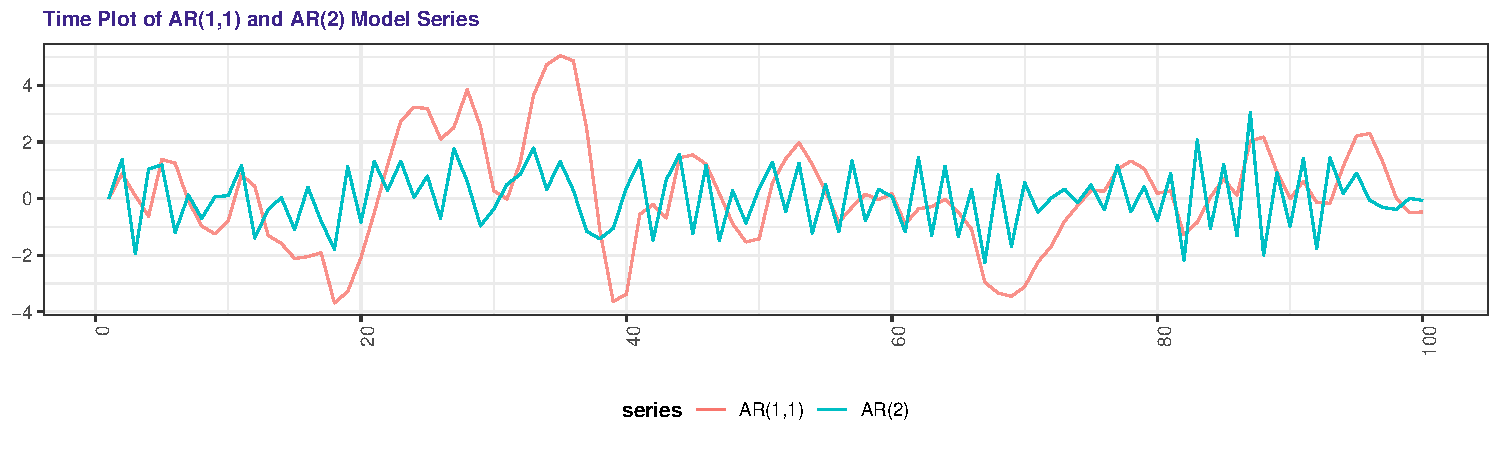
\includegraphics{homework-one_files/figure-latex/8.6g-1.pdf}

Assumptions:\\
* When \(|\theta_1|\) nears 0 in an ARMA(1,1) model, the data follows a pattern similiar to an AR(1) model.\\
* When \(|\phi_1|\) nears zero, it behaves similarly to a MA(1) model.

Our ARMA(1,1) model from 8.6(e). has parameters of \(\phi_1=0.6\) and \(\theta_1=0.6\), thus we do not expect explict AR(1) or MA(1) patterns.

Our AR(2) series shows some evidence of trend. This is likely due to the parameters of the AR(2) model from 8.6(f) being set to generate non-staionary data.

Conversely, the parameters in the ARMA(1, 1) model from 8.6(e) generate stationary.

\hypertarget{hyndman-8.8}{%
\section{Hyndman 8.8}\label{hyndman-8.8}}

Consider \texttt{austa}, the total international visitors to Australia (in millions) for the period 1980-2015.

\hypertarget{a.-use-auto.arima-to-find-an-appropriate-arima-model.-what-model-was-selected.-check-that-the-residuals-look-like-white-noise.-plot-forecasts-for-the-next-10-periods.}{%
\subsection{a. Use auto.arima() to find an appropriate ARIMA model. What model was selected. Check that the residuals look like white noise. Plot forecasts for the next 10 periods.}\label{a.-use-auto.arima-to-find-an-appropriate-arima-model.-what-model-was-selected.-check-that-the-residuals-look-like-white-noise.-plot-forecasts-for-the-next-10-periods.}}

\begin{Shaded}
\begin{Highlighting}[]
\KeywordTok{data}\NormalTok{(austa)}
\NormalTok{(fit <-}\StringTok{ }\KeywordTok{auto.arima}\NormalTok{(austa))}
\end{Highlighting}
\end{Shaded}

\begin{verbatim}
FALSE Series: austa 
FALSE ARIMA(0,1,1) with drift 
FALSE 
FALSE Coefficients:
FALSE          ma1   drift
FALSE       0.3006  0.1735
FALSE s.e.  0.1647  0.0390
FALSE 
FALSE sigma^2 estimated as 0.03376:  log likelihood=10.62
FALSE AIC=-15.24   AICc=-14.46   BIC=-10.57
\end{verbatim}

\begin{Shaded}
\begin{Highlighting}[]
\KeywordTok{residuals}\NormalTok{(fit) }\OperatorTok\StringTok{ }\KeywordTok{checkresiduals}\NormalTok{()}
\end{Highlighting}
\end{Shaded}

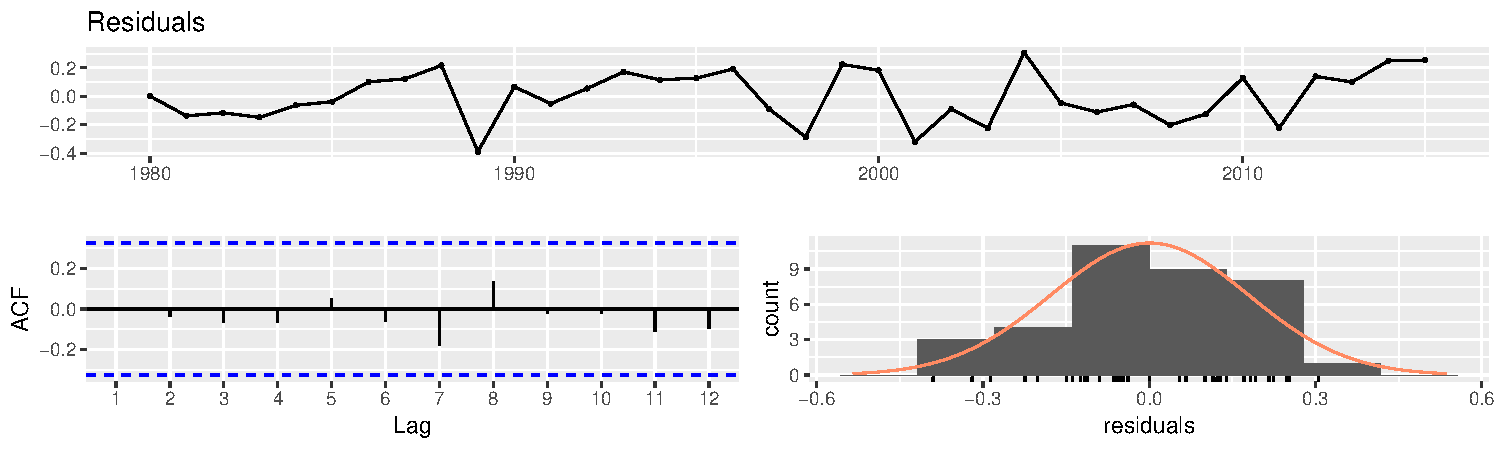
\includegraphics{homework-one_files/figure-latex/ha8.8a-1.pdf}

\begin{Shaded}
\begin{Highlighting}[]
\NormalTok{fit }\OperatorTok\StringTok{ }\KeywordTok{forecast}\NormalTok{(}\DataTypeTok{h =} \DecValTok{10}\NormalTok{) }\OperatorTok\StringTok{ }\KeywordTok{autoplot}\NormalTok{() }\OperatorTok{+}\StringTok{ }\KeywordTok{theme_bw}\NormalTok{() }\OperatorTok{+}\StringTok{ }\KeywordTok{theme}\NormalTok{()}
\end{Highlighting}
\end{Shaded}

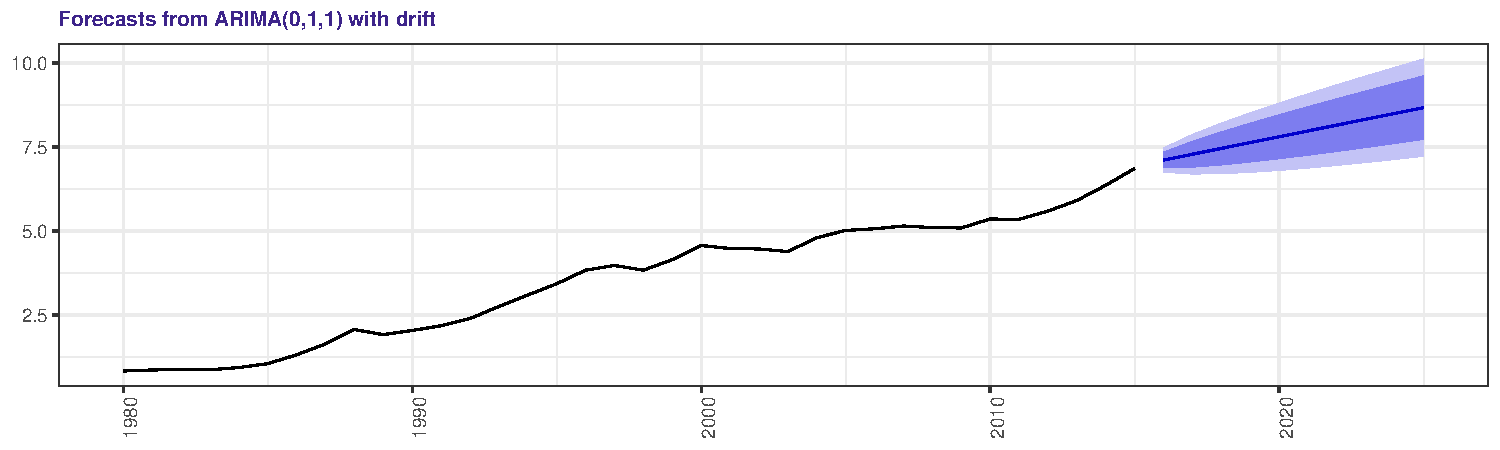
\includegraphics{homework-one_files/figure-latex/ha8.8a-2.pdf}

The results of \texttt{auto.arima()} suggest single-differencing and applying an MA(1) model with the equation \(y_t = c + y_{t-1} -.3006\epsilon_{t-1} \epsilon_t\)

\hypertarget{b.-plot-forecasts-from-an-arima011-model-with-no-drift-and-compare-these-to-part-a.-remove-the-ma-term-and-plot-again.}{%
\subsection{b. Plot forecasts from an ARIMA(0,1,1) model with no drift and compare these to part a. Remove the MA term and plot again.}\label{b.-plot-forecasts-from-an-arima011-model-with-no-drift-and-compare-these-to-part-a.-remove-the-ma-term-and-plot-again.}}

\begin{Shaded}
\begin{Highlighting}[]
\NormalTok{(fit_ma <-}\StringTok{ }\KeywordTok{Arima}\NormalTok{(austa, }\DataTypeTok{order =} \KeywordTok{c}\NormalTok{(}\DecValTok{0}\NormalTok{, }\DecValTok{1}\NormalTok{, }\DecValTok{1}\NormalTok{), }\DataTypeTok{include.mean =} \OtherTok{FALSE}\NormalTok{))}
\end{Highlighting}
\end{Shaded}

\begin{verbatim}
FALSE Series: austa 
FALSE ARIMA(0,1,1) 
FALSE 
FALSE Coefficients:
FALSE          ma1
FALSE       0.4936
FALSE s.e.  0.1265
FALSE 
FALSE sigma^2 estimated as 0.04833:  log likelihood=3.73
FALSE AIC=-3.45   AICc=-3.08   BIC=-0.34
\end{verbatim}

\begin{Shaded}
\begin{Highlighting}[]
\NormalTok{fit_ma }\OperatorTok\StringTok{ }\KeywordTok{autoplot}\NormalTok{() }\OperatorTok{+}\StringTok{ }\KeywordTok{theme_bw}\NormalTok{() }\OperatorTok{+}\StringTok{ }\KeywordTok{theme}\NormalTok{()}
\end{Highlighting}
\end{Shaded}


\includegraphics{homework-one_files/figure-latex/8.8b-1.pdf}

\begin{Shaded}
\begin{Highlighting}[]
\NormalTok{(fit_noma <-}\StringTok{ }\KeywordTok{Arima}\NormalTok{(austa, }\DataTypeTok{order =} \KeywordTok{c}\NormalTok{(}\DecValTok{0}\NormalTok{, }\DecValTok{1}\NormalTok{, }\DecValTok{0}\NormalTok{), }\DataTypeTok{include.mean =} \OtherTok{FALSE}\NormalTok{))}
\end{Highlighting}
\end{Shaded}

\begin{verbatim}
FALSE Series: austa 
FALSE ARIMA(0,1,0) 
FALSE 
FALSE sigma^2 estimated as 0.06423:  log likelihood=-1.62
FALSE AIC=5.24   AICc=5.36   BIC=6.8
\end{verbatim}

\begin{Shaded}
\begin{Highlighting}[]
\NormalTok{fit_noma }\OperatorTok\StringTok{ }\KeywordTok{autoplot}\NormalTok{() }\OperatorTok{+}\StringTok{ }\KeywordTok{theme_bw}\NormalTok{() }\OperatorTok{+}\StringTok{ }\KeywordTok{theme}\NormalTok{()}
\end{Highlighting}
\end{Shaded}


\includegraphics{homework-one_files/figure-latex/ha8.8b2-1.pdf}

\hypertarget{with-ma}{%
\subsection{With MA}\label{with-ma}}

\begin{Shaded}
\begin{Highlighting}[]
\KeywordTok{forecast}\NormalTok{(fit_ma, }\DataTypeTok{h =} \DecValTok{10}\NormalTok{) }\OperatorTok\StringTok{ }\KeywordTok{autoplot}\NormalTok{() }\OperatorTok{+}\StringTok{ }\KeywordTok{theme_bw}\NormalTok{() }\OperatorTok{+}\StringTok{ }\KeywordTok{theme}\NormalTok{()}
\end{Highlighting}
\end{Shaded}

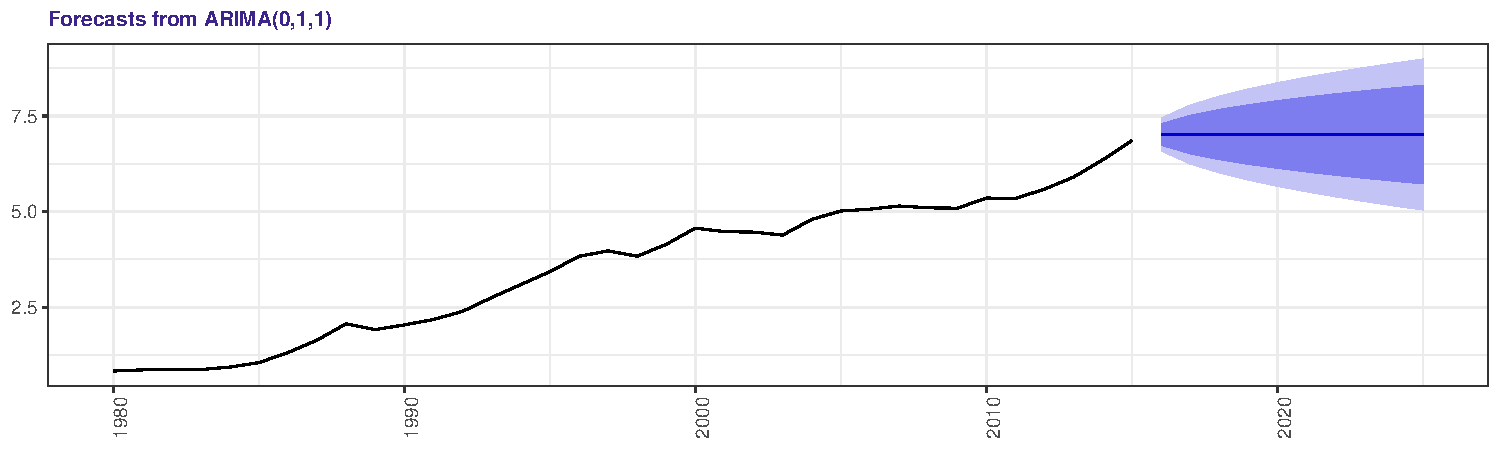
\includegraphics{homework-one_files/figure-latex/ha8.8b3-1.pdf}

\hypertarget{without-ma}{%
\subsection{Without MA}\label{without-ma}}

\begin{Shaded}
\begin{Highlighting}[]
\KeywordTok{forecast}\NormalTok{(fit_noma, }\DataTypeTok{h =} \DecValTok{10}\NormalTok{) }\OperatorTok\StringTok{ }\KeywordTok{autoplot}\NormalTok{() }\OperatorTok{+}\StringTok{ }\KeywordTok{theme_bw}\NormalTok{() }\OperatorTok{+}\StringTok{ }
\StringTok{  }\KeywordTok{theme}\NormalTok{()}
\end{Highlighting}
\end{Shaded}

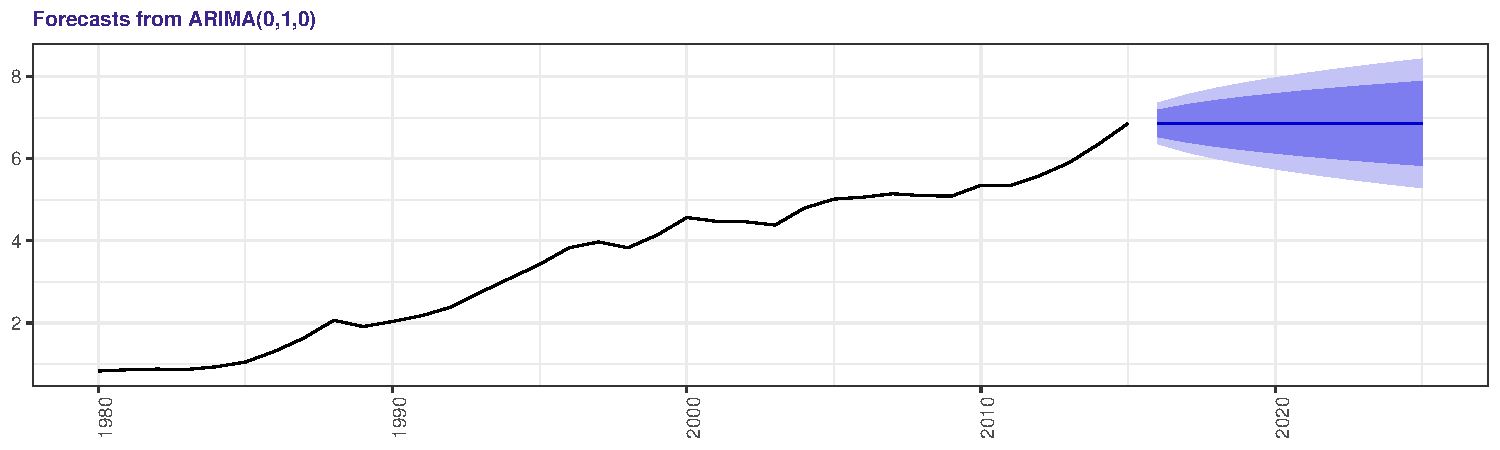
\includegraphics{homework-one_files/figure-latex/ha8.8b4-1.pdf}

\hypertarget{comparing}{%
\subsection{Comparing}\label{comparing}}

\begin{Shaded}
\begin{Highlighting}[]
\NormalTok{nm <-}\StringTok{ }\KeywordTok{forecast}\NormalTok{(fit_noma, }\DataTypeTok{h =} \DecValTok{10}\NormalTok{)}
\KeywordTok{accuracy}\NormalTok{(nm)}
\end{Highlighting}
\end{Shaded}

\begin{verbatim}
FALSE                     ME      RMSE       MAE      MPE
FALSE Training set 0.1674969 0.2498996 0.1981155 5.471861
FALSE                  MAPE      MASE      ACF1
FALSE Training set 6.479997 0.9723354 0.2583422
\end{verbatim}

\begin{Shaded}
\begin{Highlighting}[]
\NormalTok{m <-}\StringTok{ }\KeywordTok{forecast}\NormalTok{(fit_ma, }\DataTypeTok{h =} \DecValTok{10}\NormalTok{)}
\KeywordTok{accuracy}\NormalTok{(m)}
\end{Highlighting}
\end{Shaded}

\begin{verbatim}
FALSE                     ME      RMSE       MAE      MPE
FALSE Training set 0.1150344 0.2136411 0.1714887 3.817629
FALSE                  MAPE      MASE       ACF1
FALSE Training set 5.649995 0.8416532 -0.1892256
\end{verbatim}

\begin{Shaded}
\begin{Highlighting}[]
\NormalTok{difference <-}\StringTok{ }\NormalTok{m}\OperatorTok{$}\NormalTok{mean[}\DecValTok{1}\NormalTok{] }\OperatorTok{-}\StringTok{ }\NormalTok{nm}\OperatorTok{$}\NormalTok{mean[}\DecValTok{1}\NormalTok{]}
\end{Highlighting}
\end{Shaded}

\textbf{Mean of MA:} 7.015837 (the forecast value for the MA)\\
\textbf{Mean of Non-MA:} 6.858953 (the forecast value for the Non-MA)\\
\textbf{Mean Differences:} 0.156884

The two models are quite similar: their forecasts differ by .16, with approximately the same confidence windows (shifted given the different means). With a better RMSE, the (0,1,1) model may be prefereable.

\hypertarget{c.-plot-forecasts-from-an-arima213-model-with-drift.}{%
\subsection{(c.) Plot forecasts from an ARIMA(2,1,3) model with drift.}\label{c.-plot-forecasts-from-an-arima213-model-with-drift.}}

\begin{Shaded}
\begin{Highlighting}[]
\NormalTok{(fit_arima <-}\StringTok{ }\KeywordTok{Arima}\NormalTok{(austa, }\DataTypeTok{order =} \KeywordTok{c}\NormalTok{(}\DecValTok{2}\NormalTok{, }\DecValTok{1}\NormalTok{, }\DecValTok{3}\NormalTok{), }\DataTypeTok{include.drift =} \OtherTok{TRUE}\NormalTok{))}
\end{Highlighting}
\end{Shaded}

\begin{verbatim}
FALSE Series: austa 
FALSE ARIMA(2,1,3) with drift 
FALSE 
FALSE Coefficients:
FALSE          ar1      ar2      ma1     ma2     ma3   drift
FALSE       1.7648  -0.8513  -1.7684  0.5571  0.2224  0.1725
FALSE s.e.  0.1136   0.1182   0.2433  0.4351  0.2150  0.0051
FALSE 
FALSE sigma^2 estimated as 0.0276:  log likelihood=13.72
FALSE AIC=-13.44   AICc=-9.29   BIC=-2.55
\end{verbatim}

\begin{Shaded}
\begin{Highlighting}[]
\NormalTok{fit_arima }\OperatorTok\StringTok{ }\KeywordTok{autoplot}\NormalTok{() }\OperatorTok{+}\StringTok{ }\KeywordTok{theme_bw}\NormalTok{() }\OperatorTok{+}\StringTok{ }\KeywordTok{theme}\NormalTok{()}
\end{Highlighting}
\end{Shaded}

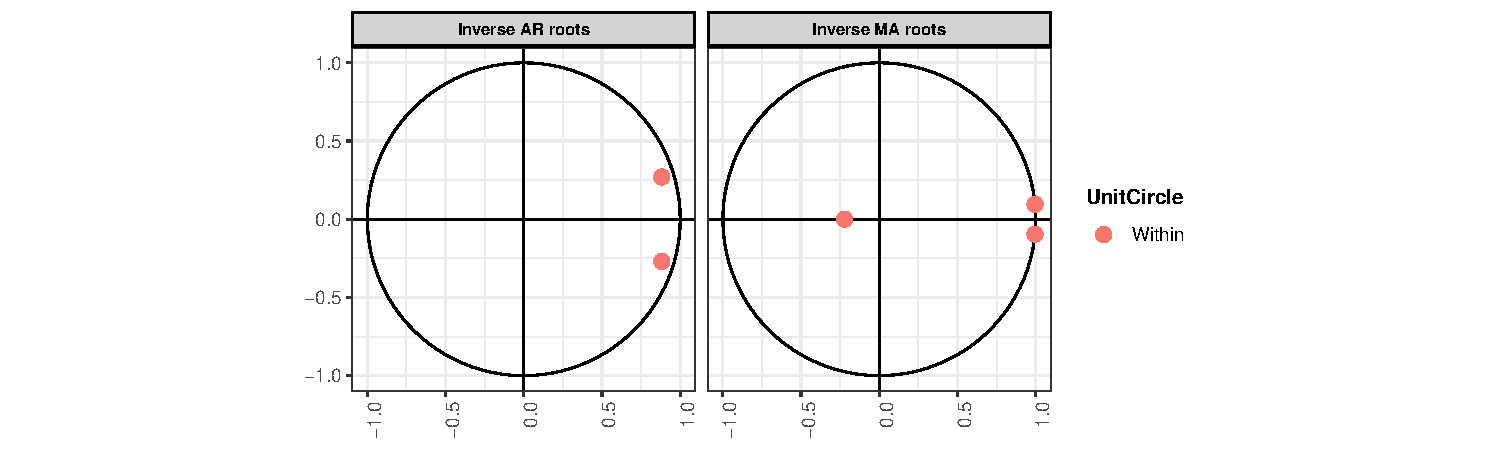
\includegraphics{homework-one_files/figure-latex/8.8c1-1.pdf}

\begin{Shaded}
\begin{Highlighting}[]
\NormalTok{fit_arima }\OperatorTok\StringTok{ }\KeywordTok{forecast}\NormalTok{(}\DataTypeTok{h =} \DecValTok{10}\NormalTok{) }\OperatorTok\StringTok{ }\KeywordTok{autoplot}\NormalTok{() }\OperatorTok{+}\StringTok{ }\KeywordTok{theme_bw}\NormalTok{() }\OperatorTok{+}\StringTok{ }
\StringTok{  }\KeywordTok{theme}\NormalTok{()}
\end{Highlighting}
\end{Shaded}

\includegraphics{homework-one_files/figure-latex/8.8c1-2.pdf}

\begin{Shaded}
\begin{Highlighting}[]
\KeywordTok{accuracy}\NormalTok{(}\KeywordTok{forecast}\NormalTok{(fit_arima))}
\end{Highlighting}
\end{Shaded}

\begin{verbatim}
FALSE                        ME      RMSE      MAE       MPE
FALSE Training set -0.004129818 0.1491068 0.114857 -1.203567
FALSE                  MAPE      MASE        ACF1
FALSE Training set 4.326425 0.5637093 -0.01736817
\end{verbatim}

Visually this model seems to improve the forecsts. It takes into account the upwasrd trend missing in the (0,1,0) and (0,1,1) forecasts; it offers a much tighter confidence window throughout the prediction range; and, lastly, its RMSE of .14 suggests a better forecast.

\begin{quote}
Remove the constant and see what happens
\end{quote}

\begin{Shaded}
\begin{Highlighting}[]
\NormalTok{(fit_arima <-}\StringTok{ }\KeywordTok{Arima}\NormalTok{(austa, }\DataTypeTok{order =} \KeywordTok{c}\NormalTok{(}\DecValTok{2}\NormalTok{, }\DecValTok{1}\NormalTok{, }\DecValTok{3}\NormalTok{), }\DataTypeTok{include.constant =} \OtherTok{FALSE}\NormalTok{))}
\NormalTok{fit_arima }\OperatorTok\StringTok{ }\KeywordTok{autoplot}\NormalTok{()}
\end{Highlighting}
\end{Shaded}

In the current state, the coefficients for the AR component breed non-stationarity, such that the model throws an error.

\texttt{Error\ in\ stats::arima(x\ =\ x,\ order\ =\ order,\ seasonal\ =\ seasonal,\ include.mean\ =\ include.mean,\ :\ non-stationary\ AR\ part\ from\ CSS}

This can be corrected by switching to the traditional ``Maximum Likelihood'' method or ``CSS'' method.

\begin{Shaded}
\begin{Highlighting}[]
\NormalTok{(fit_arima <-}\StringTok{ }\KeywordTok{Arima}\NormalTok{(austa, }\DataTypeTok{order =} \KeywordTok{c}\NormalTok{(}\DecValTok{2}\NormalTok{, }\DecValTok{1}\NormalTok{, }\DecValTok{3}\NormalTok{), }\DataTypeTok{include.constant =} \OtherTok{FALSE}\NormalTok{, }
  \DataTypeTok{method =} \StringTok{"ML"}\NormalTok{))}
\end{Highlighting}
\end{Shaded}

\begin{verbatim}
FALSE Series: austa 
FALSE ARIMA(2,1,3) 
FALSE 
FALSE Coefficients:
FALSE          ar1     ar2     ma1      ma2      ma3
FALSE       0.0004  0.9996  0.4633  -0.9893  -0.4625
FALSE s.e.  0.0031  0.0031  0.2283   0.0329   0.2261
FALSE 
FALSE sigma^2 estimated as 0.03568:  log likelihood=9.24
FALSE AIC=-6.48   AICc=-3.48   BIC=2.85
\end{verbatim}

\begin{Shaded}
\begin{Highlighting}[]
\NormalTok{fit_arima }\OperatorTok\StringTok{ }\KeywordTok{autoplot}\NormalTok{() }\OperatorTok{+}\StringTok{ }\KeywordTok{theme_bw}\NormalTok{() }\OperatorTok{+}\StringTok{ }\KeywordTok{theme}\NormalTok{()}
\end{Highlighting}
\end{Shaded}

\includegraphics{homework-one_files/figure-latex/8.8c3-1.pdf}

\begin{Shaded}
\begin{Highlighting}[]
\NormalTok{fit_arima }\OperatorTok\StringTok{ }\KeywordTok{forecast}\NormalTok{(}\DataTypeTok{h =} \DecValTok{10}\NormalTok{) }\OperatorTok\StringTok{ }\KeywordTok{autoplot}\NormalTok{() }\OperatorTok{+}\StringTok{ }\KeywordTok{theme_bw}\NormalTok{() }\OperatorTok{+}\StringTok{ }
\StringTok{  }\KeywordTok{theme}\NormalTok{()}
\end{Highlighting}
\end{Shaded}

\includegraphics{homework-one_files/figure-latex/8.8c3-2.pdf}

\begin{Shaded}
\begin{Highlighting}[]
\KeywordTok{accuracy}\NormalTok{(}\KeywordTok{forecast}\NormalTok{(fit_arima))}
\end{Highlighting}
\end{Shaded}

\begin{verbatim}
FALSE                      ME      RMSE       MAE      MPE
FALSE Training set 0.03972287 0.1724412 0.1402048 1.685829
FALSE                  MAPE      MASE        ACF1
FALSE Training set 4.592996 0.6881143 -0.07513543
\end{verbatim}

This approach leads to a much wider confidence interval and unit roots moved to the extremes of the acceptable stationary range (-1,0) and (1,0) for both the MA and AR components (suggesting only marginal stationarity).

Including the constant term does seem to improve model performance and yield a more compact prediction interval.

In order to compare apples to apples, we also used the `ML' method on the model when we add the drift.

\begin{Shaded}
\begin{Highlighting}[]
\NormalTok{(fit_arima <-}\StringTok{ }\KeywordTok{Arima}\NormalTok{(austa, }\DataTypeTok{order =} \KeywordTok{c}\NormalTok{(}\DecValTok{2}\NormalTok{, }\DecValTok{1}\NormalTok{, }\DecValTok{3}\NormalTok{), }\DataTypeTok{include.drift =} \OtherTok{TRUE}\NormalTok{, }
  \DataTypeTok{method =} \StringTok{"ML"}\NormalTok{))}
\end{Highlighting}
\end{Shaded}

\begin{verbatim}
FALSE Series: austa 
FALSE ARIMA(2,1,3) with drift 
FALSE 
FALSE Coefficients:
FALSE          ar1      ar2      ma1     ma2     ma3   drift
FALSE       1.7648  -0.8513  -1.7684  0.5571  0.2224  0.1725
FALSE s.e.  0.1136   0.1182   0.2433  0.4351  0.2150  0.0051
FALSE 
FALSE sigma^2 estimated as 0.0276:  log likelihood=13.72
FALSE AIC=-13.44   AICc=-9.29   BIC=-2.55
\end{verbatim}

\begin{Shaded}
\begin{Highlighting}[]
\NormalTok{fit_arima }\OperatorTok\StringTok{ }\KeywordTok{autoplot}\NormalTok{() }\OperatorTok{+}\StringTok{ }\KeywordTok{theme_bw}\NormalTok{() }\OperatorTok{+}\StringTok{ }\KeywordTok{theme}\NormalTok{()}
\end{Highlighting}
\end{Shaded}

\includegraphics{homework-one_files/figure-latex/ha8.8c4-1.pdf}

\begin{Shaded}
\begin{Highlighting}[]
\NormalTok{fit_arima }\OperatorTok\StringTok{ }\KeywordTok{forecast}\NormalTok{(}\DataTypeTok{h =} \DecValTok{10}\NormalTok{) }\OperatorTok\StringTok{ }\KeywordTok{autoplot}\NormalTok{() }\OperatorTok{+}\StringTok{ }\KeywordTok{theme_bw}\NormalTok{() }\OperatorTok{+}\StringTok{ }
\StringTok{  }\KeywordTok{theme}\NormalTok{()}
\end{Highlighting}
\end{Shaded}

\includegraphics{homework-one_files/figure-latex/ha8.8c4-2.pdf}

\begin{Shaded}
\begin{Highlighting}[]
\KeywordTok{accuracy}\NormalTok{(}\KeywordTok{forecast}\NormalTok{(fit_arima))}
\end{Highlighting}
\end{Shaded}

\begin{verbatim}
FALSE                        ME      RMSE      MAE       MPE
FALSE Training set -0.004129818 0.1491068 0.114857 -1.203567
FALSE                  MAPE      MASE        ACF1
FALSE Training set 4.326425 0.5637093 -0.01736817
\end{verbatim}

This forecast is very similar to the original (2,1,3) model, but it compares more favorably in terms of training error metrics. The AICc is considerably lower with constant (and drift) than without, as are the forecasting RMSE and resulting prediction interval. In short, it makes sense to allow for drift.

\hypertarget{d.-plot-forecasts-from-an-arima001-model-with-a-constant.-remove-the-ma-term-and-plot-again.}{%
\subsection{(d.) Plot forecasts from an ARIMA(0,0,1) model with a constant. Remove the MA term and plot again.}\label{d.-plot-forecasts-from-an-arima001-model-with-a-constant.-remove-the-ma-term-and-plot-again.}}

\begin{Shaded}
\begin{Highlighting}[]
\NormalTok{(fit_ma <-}\StringTok{ }\KeywordTok{Arima}\NormalTok{(austa, }\DataTypeTok{order =} \KeywordTok{c}\NormalTok{(}\DecValTok{0}\NormalTok{, }\DecValTok{0}\NormalTok{, }\DecValTok{1}\NormalTok{), }\DataTypeTok{include.mean =} \OtherTok{TRUE}\NormalTok{))}
\end{Highlighting}
\end{Shaded}

\begin{verbatim}
FALSE Series: austa 
FALSE ARIMA(0,0,1) with non-zero mean 
FALSE 
FALSE Coefficients:
FALSE          ma1    mean
FALSE       1.0000  3.5515
FALSE s.e.  0.0907  0.3090
FALSE 
FALSE sigma^2 estimated as 0.9347:  log likelihood=-50.64
FALSE AIC=107.28   AICc=108.03   BIC=112.04
\end{verbatim}

\begin{Shaded}
\begin{Highlighting}[]
\NormalTok{fit_ma }\OperatorTok\StringTok{ }\KeywordTok{autoplot}\NormalTok{() }\OperatorTok{+}\StringTok{ }\KeywordTok{theme_bw}\NormalTok{() }\OperatorTok{+}\StringTok{ }\KeywordTok{theme}\NormalTok{()}
\end{Highlighting}
\end{Shaded}

\includegraphics{homework-one_files/figure-latex/ha8.8d1-1.pdf}

\begin{Shaded}
\begin{Highlighting}[]
\NormalTok{(fit_noma <-}\StringTok{ }\KeywordTok{Arima}\NormalTok{(austa, }\DataTypeTok{order =} \KeywordTok{c}\NormalTok{(}\DecValTok{0}\NormalTok{, }\DecValTok{0}\NormalTok{, }\DecValTok{0}\NormalTok{), }\DataTypeTok{include.mean =} \OtherTok{FALSE}\NormalTok{))}
\end{Highlighting}
\end{Shaded}

\begin{verbatim}
FALSE Series: austa 
FALSE ARIMA(0,0,0) with zero mean 
FALSE 
FALSE sigma^2 estimated as 15.72:  log likelihood=-100.67
FALSE AIC=203.34   AICc=203.46   BIC=204.93
\end{verbatim}

\begin{Shaded}
\begin{Highlighting}[]
\NormalTok{fit_noma }\OperatorTok\StringTok{ }\KeywordTok{autoplot}\NormalTok{() }\OperatorTok{+}\StringTok{ }\KeywordTok{theme_bw}\NormalTok{() }\OperatorTok{+}\StringTok{ }\KeywordTok{theme}\NormalTok{()}
\end{Highlighting}
\end{Shaded}

\includegraphics{homework-one_files/figure-latex/ha8.8d1-2.pdf}

\hypertarget{with-ma-1}{%
\subsection{With MA}\label{with-ma-1}}

\begin{Shaded}
\begin{Highlighting}[]
\KeywordTok{forecast}\NormalTok{(fit_ma, }\DataTypeTok{h =} \DecValTok{10}\NormalTok{) }\OperatorTok\StringTok{ }\KeywordTok{autoplot}\NormalTok{() }\OperatorTok{+}\StringTok{ }\KeywordTok{theme_bw}\NormalTok{() }\OperatorTok{+}\StringTok{ }\KeywordTok{theme}\NormalTok{()}
\end{Highlighting}
\end{Shaded}

\includegraphics{homework-one_files/figure-latex/ha8.8d2-1.pdf}

\hypertarget{without-ma-1}{%
\subsection{Without MA}\label{without-ma-1}}

\begin{Shaded}
\begin{Highlighting}[]
\KeywordTok{forecast}\NormalTok{(fit_noma, }\DataTypeTok{h =} \DecValTok{10}\NormalTok{) }\OperatorTok\StringTok{ }\KeywordTok{autoplot}\NormalTok{() }\OperatorTok{+}\StringTok{ }\KeywordTok{theme_bw}\NormalTok{() }\OperatorTok{+}\StringTok{ }
\StringTok{  }\KeywordTok{theme}\NormalTok{()}
\end{Highlighting}
\end{Shaded}

\includegraphics{homework-one_files/figure-latex/ha8.8d3-1.pdf}

Even without examination of error measures its evident that these forecasts are not particularly useful. The moving average forecast begins accounting for the trend, but then deteriorates to the mean; the (0,0,0) model simply predicts a static mean over an obviously more complex time series than the forecasts reflect.

\hypertarget{accuracy}{%
\subsection{Accuracy}\label{accuracy}}

\begin{Shaded}
\begin{Highlighting}[]
\KeywordTok{accuracy}\NormalTok{(}\KeywordTok{forecast}\NormalTok{(fit_ma, }\DataTypeTok{h =} \DecValTok{10}\NormalTok{))}
\end{Highlighting}
\end{Shaded}

\begin{verbatim}
FALSE                      ME      RMSE       MAE       MPE
FALSE Training set 0.01997167 0.9395462 0.8063899 -26.87733
FALSE                  MAPE     MASE      ACF1
FALSE Training set 42.56419 3.957698 0.8109528
\end{verbatim}

\begin{Shaded}
\begin{Highlighting}[]
\KeywordTok{accuracy}\NormalTok{(}\KeywordTok{forecast}\NormalTok{(fit_noma, }\DataTypeTok{h =} \DecValTok{10}\NormalTok{))}
\end{Highlighting}
\end{Shaded}

\begin{verbatim}
FALSE                    ME     RMSE      MAE MPE MAPE
FALSE Training set 3.541428 3.964979 3.541428 100  100
FALSE                  MASE      ACF1
FALSE Training set 17.38105 0.9099807
\end{verbatim}

This assessment gains further support given the high RMSE for the MA(1) and even higher RMSE for the (0,0,0) model. Neither are particularly useful forecasts.

\hypertarget{e.-plot-forecasts-from-an-arima021-model-with-no-constant.}{%
\subsection{(e.) Plot forecasts from an ARIMA(0,2,1) model with no constant.}\label{e.-plot-forecasts-from-an-arima021-model-with-no-constant.}}

\begin{Shaded}
\begin{Highlighting}[]
\NormalTok{(fit_ma <-}\StringTok{ }\KeywordTok{Arima}\NormalTok{(austa, }\DataTypeTok{order =} \KeywordTok{c}\NormalTok{(}\DecValTok{0}\NormalTok{, }\DecValTok{2}\NormalTok{, }\DecValTok{1}\NormalTok{), }\DataTypeTok{include.mean =} \OtherTok{TRUE}\NormalTok{))}
\end{Highlighting}
\end{Shaded}

\begin{verbatim}
FALSE Series: austa 
FALSE ARIMA(0,2,1) 
FALSE 
FALSE Coefficients:
FALSE           ma1
FALSE       -0.7263
FALSE s.e.   0.2277
FALSE 
FALSE sigma^2 estimated as 0.03969:  log likelihood=6.74
FALSE AIC=-9.48   AICc=-9.09   BIC=-6.43
\end{verbatim}

\begin{Shaded}
\begin{Highlighting}[]
\NormalTok{fit_ma }\OperatorTok\StringTok{ }\KeywordTok{autoplot}\NormalTok{() }\OperatorTok{+}\StringTok{ }\KeywordTok{theme_bw}\NormalTok{() }\OperatorTok{+}\StringTok{ }\KeywordTok{theme}\NormalTok{()}
\end{Highlighting}
\end{Shaded}

\includegraphics{homework-one_files/figure-latex/ha8.8e-1.pdf}

\begin{Shaded}
\begin{Highlighting}[]
\KeywordTok{forecast}\NormalTok{(fit_ma, }\DataTypeTok{h =} \DecValTok{10}\NormalTok{) }\OperatorTok\StringTok{ }\KeywordTok{autoplot}\NormalTok{() }\OperatorTok{+}\StringTok{ }\KeywordTok{theme_bw}\NormalTok{() }\OperatorTok{+}\StringTok{ }\KeywordTok{theme}\NormalTok{()}
\end{Highlighting}
\end{Shaded}

\includegraphics{homework-one_files/figure-latex/ha8.8e-2.pdf}

\begin{Shaded}
\begin{Highlighting}[]
\KeywordTok{accuracy}\NormalTok{(}\KeywordTok{forecast}\NormalTok{(fit_ma, }\DataTypeTok{h =} \DecValTok{10}\NormalTok{))}
\end{Highlighting}
\end{Shaded}

\begin{verbatim}
FALSE                      ME      RMSE       MAE      MPE
FALSE Training set 0.02907781 0.1907537 0.1567877 1.216128
FALSE                  MAPE      MASE      ACF1
FALSE Training set 4.984081 0.7695018 0.1284994
\end{verbatim}

Based on RMSE alone, this would seem a go-to model when compared with the (0,0,1), (0,0,0) and (0,1,1) models. It is close to as good as the (2,1,3) without drift, which had an RMSE of .17; however, the (2,1,3) with drift had the overall best RMSE of .14.

Given that the (2,1,3) model also had a tighter confidence window it makes sense to consider that there is some autoregression in this series and use the full ARIMA(2,1,3) with drift in predicting over this data set.

\bibliography{book.bib,packages.bib}


\end{document}
